% ==== Document Class & Packages =====
\documentclass[12pt,hidelinks]{article}
	\usepackage[explicit]{titlesec}
	\usepackage{titletoc}
	\usepackage{tocloft}
	\usepackage{charter}
	\usepackage[many]{tcolorbox}
	\usepackage{amsmath}
	\usepackage{graphicx}
	\usepackage{xcolor}
	\usepackage{tikz,lipsum,lmodern}
	\usetikzlibrary{calc}
	\usepackage[portuges]{babel}
	\usepackage[utf8]{inputenc}
	\usepackage{fancyhdr}
	\usepackage{mathrsfs}
	\usepackage{empheq}
	\usepackage{fourier}% change to lmodern if fourier is no available
	\usepackage{wrapfig}
	\usepackage{fancyref}
	\usepackage{hyperref}
	\usepackage{cleveref}
	\usepackage{listings}
	\usepackage{varwidth}
	\usepackage{longfbox}
	\usepackage{geometry}
    \usepackage{enumerate}
	\usepackage{marginnote}
	\usepackage{minted}
	\usepackage{subcaption}
	\usemintedstyle{borland}
	\tcbuselibrary{theorems}
	\tcbuselibrary{breakable, skins}
	\tcbuselibrary{listings, documentation}
	\geometry{
		a4paper,
		left=30mm,
		right=20mm,
		top=30mm}
% ========= Path to images ============
%   - Direct the computer on the path 
% 	  to the folder containg the images
% =====================================
\graphicspath{{./images/}}
% ============= Macros ================
\newcommand{\fillin}{\underline{\hspace{.75in}}{\;}}
\newcommand{\solution}{\textcolor{mordantred19}{Solution:}}
\setlength{\parindent}{22pt}
\addto{\captionsenglish}{\renewcommand*{\contentsname}{Table of Contents}}
\linespread{1.2}
% ======== Footers & Headers ==========
\cfoot{\thepage}
\chead{}\rhead{}\lhead{}
% =====================================
\renewcommand{\thesection}{\arabic{section}}
\newcommand\sectionnumfont{% font specification for the number
	\fontsize{380}{130}\color{myblueii}\selectfont}
\newcommand\sectionnamefont{% font specification for the name "PART"
	\normalfont\color{white}\scshape\small\bfseries }
% ============= Colors ================
% ----- Red -----
\definecolor{mordantred19}{rgb}{0.68, 0.05, 0.0}
% ----- Blue -----
\definecolor{st.patrick\'sblue}{rgb}{0.14, 0.16, 0.48}
\definecolor{teal}{rgb}{0.0, 0.5, 0.5}
\definecolor{beaublue}{rgb}{0.74, 0.83, 0.9}
\definecolor{mybluei}{RGB}{0,173,239}
\definecolor{myblueii}{RGB}{63,200,244}
\definecolor{myblueiii}{RGB}{199,234,253}
% ---- Yellow ----
\definecolor{blond}{rgb}{0.98, 0.94, 0.75}
\definecolor{cream}{rgb}{1.0, 0.99, 0.82}
% ----- Green ------
\definecolor{emerald}{rgb}{0.31, 0.78, 0.47}
\definecolor{darkspringgreen}{rgb}{0.09, 0.45, 0.27}
% ---- White -----
\definecolor{ghostwhite}{rgb}{0.97, 0.97, 1.0}
\definecolor{splashedwhite}{rgb}{1.0, 0.99, 1.0}
% ---- Grey -----
\definecolor{whitesmoke}{rgb}{0.96, 0.96, 0.96}
\definecolor{lightgray}{rgb}{0.92, 0.92, 0.92}
\definecolor{floralwhite}{rgb}{1.0, 0.98, 0.94}
% ========= Part Format ==========
\titleformat{\section}
{\normalfont\huge\filleft}
{}
{20pt}
{\begin{tikzpicture}[remember picture,overlay]
	\fill[myblueiii] 
	(current page.north west) rectangle ([yshift=-13cm]current page.north east);   
\node[
	fill=mybluei,
	text width=2\paperwidth,
	rounded corners=6cm,
	text depth=18cm,
	anchor=center,
	inner sep=0pt] at (current page.north east) (parttop)
	{\thepart};%
\node[
	anchor=south east,
	inner sep=0pt,
	outer sep=0pt] (partnum) at ([xshift=-20pt]parttop.south) 
	{\sectionnumfont\thesection};
\node[
	anchor=south,
	inner sep=0pt] (partname) at ([yshift=2pt]partnum.south)   
	{\sectionnamefont SECTION};
\node[
	anchor=north east,
	align=right,
	inner xsep=0pt] at ([yshift=-0.5cm]partname.east|-partnum.south) 
	{\parbox{.7\textwidth}{\raggedleft#1}};
\end{tikzpicture}%
}
% ========= Hyper Ref ===========
\hypersetup{
	colorlinks,
	linkcolor={red!50!black},
	citecolor={blue!50!black},
	urlcolor={blue!80!black}
}
% ========= Example Boxes =============
\tcbset{
	defstyle/.style={
		fonttitle=\bfseries\upshape, 
		fontupper=\slshape,
		arc=0mm, 
		beamer,
		colback=blue!5!white,
		colframe=blue!75!black},
	theostyle/.style={
		fonttitle=\bfseries\upshape, 
		fontupper=\slshape,
		colback=red!10!white,
		colframe=red!75!black},
	visualstyle/.style={
		height=6.5cm,
		breakable,
		enhanced,
		leftrule=0pt,
		rightrule=0pt,
		bottomrule=0pt,
		outer arc=0pt,
		arc=0pt,
		colframe=mordantred19,
		colback=lightgray,
		attach boxed title to top left,
		boxed title style={
			colback=mordantred19,
			outer arc=0pt,
			arc=0pt,
			top=3pt,
			bottom=3pt,
		},
		fonttitle=\sffamily,},
	discussionstyle/.style={
		height=6.5cm,
		breakable,
		enhanced,
		rightrule=0pt,
		toprule=0pt,
		outer arc=0pt,
		arc=0pt,
		colframe=mordantred19,
		colback=lightgray,
		attach boxed title to top left,
		boxed title style={
			colback=mordantred19,
			outer arc=0pt,
			arc=0pt,
			top=3pt,
			bottom=3pt,
		},
		fonttitle=\sffamily},
	mystyle/.style={
		height=6.5cm,
		breakable,
		enhanced,
		rightrule=0pt,
		leftrule=0pt,
		bottomrule=0pt,
		outer arc=0pt,
		arc=0pt,
		colframe=mordantred19,
		colback=lightgray,
		attach boxed title to top left,
		boxed title style={
			colback=mordantred19,
			outer arc=0pt,
			arc=0pt,
			top=3pt,
			bottom=3pt,
		},
		fonttitle=\sffamily},
	aastyle/.style={
			height=3.5cm,
			enhanced,
			colframe=teal,
			colback=lightgray,
			colbacktitle=floralwhite,
			fonttitle=\bfseries,
			coltitle=black,
		attach boxed title to top center={
	  		yshift=-0.25mm-\tcboxedtitleheight/2,
	   		yshifttext=2mm-\tcboxedtitleheight/2}, 
		boxed title style={boxrule=0.5mm,
			frame code={ \path[tcb fill frame] ([xshift=-4mm]frame.west)
				-- (frame.north west) -- (frame.north east) -- ([xshift=4mm]frame.east)
				-- (frame.south east) -- (frame.south west) -- cycle; },
			interior code={ 
				\path[tcb fill interior] ([xshift=-2mm]interior.west)
				-- (interior.north west) -- (interior.north east)
				-- ([xshift=2mm]interior.east) -- (interior.south east) -- (interior.south west)
				-- cycle;} }
				},
	examstyle/.style={
		height=9.5cm,
		breakable,
		enhanced,
		rightrule=0pt,
		leftrule=0pt,
		bottomrule=0pt,
		outer arc=0pt,
		arc=0pt,
		colframe=mordantred19,
		colback=lightgray,
		attach boxed title to top left,
		boxed title style={
			colback=mordantred19,
			outer arc=0pt,
			arc=0pt,
			top=3pt,
			bottom=3pt,
		},
		fonttitle=\sffamily},
	doc head command={
		interior style={
			fill,
			left color=yellow!20!white, 
			right color=white}},
	doc head environment={
		boxsep=4pt,
		arc=2pt,
		colback=yellow!30!white,
		},
	doclang/environment content=text
}
% ============= Boxes ================
\newtcolorbox[auto counter,number within=section]{example}[1][]{
	mystyle,
	title=Example~\thetcbcounter,
	overlay unbroken and first={
		\path
		let
		\p1=(title.north east),
		\p2=(frame.north east)
		in
		node[anchor=
			west,
			font=\sffamily,
			color=st.patrick\'sblue,
			text width=\x2-\x1] 
		at (title.east) {#1};
	}
}
\newtcolorbox[auto counter,number within=section]{longexample}[1][]{
	examstyle,
	title=Example~\thetcbcounter,
	overlay unbroken and first={
		\path
		let
		\p1=(title.north east),
		\p2=(frame.north east)
		in
		node[anchor=
		west,
		font=\sffamily,
		color=st.patrick\'sblue,
		text width=\x2-\x1] 
		at (title.east) {#1};
	}
}
\newtcolorbox[auto counter,number within=section]{example2}[1][]{
	aastyle,
	title=Example~\thetcbcounter,{}
}
\newtcolorbox[auto counter,number within=section]{discussion}[1][]{
	discussionstyle,
	title=Discussion~\thetcbcounter,
	overlay unbroken and first={
		\path
		let
		\p1=(title.north east),
		\p2=(frame.north east)
		in
		node[anchor=
		west,
		font=\sffamily,
		color=st.patrick\'sblue,
		text width=\x2-\x1] 
		at (title.east) {#1};
	}
}
\newtcolorbox[auto counter,number within=section]{visualization}[1][]{
	visualstyle,
	title=Visualization~\thetcbcounter,
	overlay unbroken and first={
		\path
		let
		\p1=(title.north east),
		\p2=(frame.north east)
		in
		node[anchor=
		west,
		font=\sffamily,
		color=st.patrick\'sblue,
		text width=\x2-\x1] 
		at (title.east) {#1};
	}
}
% --------- Theorems ---------
\newtcbtheorem[number within=subsection,crefname={definition}{definitions}]%
	{Definition}{Definition}{defstyle}{def}%
\newtcbtheorem[use counter from=Definition,crefname={theorem}{theorems}]%
	{Theorem}{Theorem}{theostyle}{theo}
	%
\newtcbtheorem[use counter from=Definition]{theo}{Theorem}%
{
	theorem style=plain,
	enhanced,
	colframe=blue!50!black,
	colback=yellow!20!white,
	coltitle=red!50!black,
	fonttitle=\upshape\bfseries,
	fontupper=\itshape,
	drop fuzzy shadow=blue!50!black!50!white,
	boxrule=0.4pt}{theo}
\newtcbtheorem[use counter from=Definition]{DashedDefinition}{Definition}%
 {
 	enhanced,
 	frame empty,
 	interior empty,
 	colframe=darkspringgreen!50!white,
	coltitle=darkspringgreen!50!black,
	fonttitle=\bfseries,
	colbacktitle=darkspringgreen!15!white,
	borderline={0.5mm}{0mm}{darkspringgreen!15!white},
	borderline={0.5mm}{0mm}{darkspringgreen!50!white,dashed},
	attach boxed title to top center={yshift=-2mm},
	boxed title style={boxrule=0.4pt},
	varwidth boxed title}{theo}
%%%%%%%%%%%%%%%%%%%%%%%%%%%%%%%%%%%%%%%%
\newtcblisting[auto counter,number within=section]{disexam}{
	skin=bicolor,
	colback=white!30!beaublue,
	colbacklower=white,
	colframe=black,
	before skip=\medskipamount,
	after skip=\medskipamount,
	fontlower=\footnotesize,
	listing options={style=tcblatex,texcsstyle=*\color{red!70!black}},}
	

	
%%%%%%%%%%%%%%%%%%%%%%%%%%%%%%%%%%%%%%%

\begin{document}
\begin{titlepage}
	\centering % Center everything on the title page
	\scshape % Use small caps for all text on the title page
	\vspace*{1.5\baselineskip} % White space at the top of the page
% ===================
%	Title Section 	
% ===================

	\rule{13cm}{1.6pt}\vspace*{-\baselineskip}\vspace*{2pt} % Thick horizontal rule
	\rule{13cm}{0.4pt} % Thin horizontal rule
	
		\vspace{0.75\baselineskip} % Whitespace above the title
% ========== Title ===============	
	{	\Huge Manual do Dataverse\\ 
			\vspace{4mm}}
% ======================================
		\vspace{0.75\baselineskip} % Whitespace below the title
	\rule{13cm}{0.4pt}\vspace*{-\baselineskip}\vspace{3.2pt} % Thin horizontal rule
	\rule{13cm}{1.6pt} % Thick horizontal rule
	
		\vspace{1.75\baselineskip} % Whitespace after the title block
% =================
%	Information	
% =================
	{\large Lucas N. Paganine\\ Vanderlino C. Barreto Neto \\
		\vspace*{1.2\baselineskip}
	lucaspaganine@ibict.br\\ vanderlinoneto@ibict.br} \\https://www.overleaf.com/read/vqytysgjbznd\\
	\vspace*{1.2\baselineskip}
	
	Revisão por:\\
	\small Luciana dos Santos Nahuz\\
	
	
	
	\vfill
\end{titlepage}
%%%%%%%%%%%%%%%%%%%%%%%%%%%%%%%%%%%%%%%%%%%%%%%%%%%%%%%%%%%

\listoffigures

\newpage

\listoftables

\newpage

\tableofcontents
\vfill
\newpage
\newgeometry{
	left=29mm, 
	right=29mm, 
	top=20mm, 
	bottom=15mm}
%%%%%%%%%%%%%%%%%%%%%%%%%%%%%%%%%%%%%%%%%%%%%%%%%%%%%%%%%%%
%\section{Manual de instalação}
%\vspace{10.5cm}

\section{INSTALAÇÃO}
\vspace{10.5cm}

    \subsection{Pré instalações}

        \subsubsection{Preparação do Servidor}
        
            \qquad O sistema operacional utilizado no servidor será o Debian 9. Esse sistema operacional foi escolhido por ser um dos mais utilizado em 
 Add comment
  Recompile
3
 servidores de instituições acadêmicas. Os programas são instalados utilizando o programa gestor de pacotes Apt, contudo, por conta de problemas de compatibilidade, alguns programas serão instalados \\manualmente.
            
            É necessário a autorização de administrador ou de superusuário(\textit{root}) em algumas etapas da instalação, com isso, recomenda-se estar logado como \textit{root} durante a instalação. Caso seja necessário a mudança de usuário, haverá uma instrução. Para acessar como superusuário, tendo conhecimento da senha, pode-se usar o comando \textbf{su}.
            \begin{minted}{bash}
    su -
            \end{minted}
            Quando não é conhecido a senha de root, porém o usuário está no grupo de sudores do servidor, pode-se usar o comando a seguir.
            \begin{minted}{bash}
    sudo su
            \end{minted}
            
            A primeira coisa a se fazer, depois de acessar como superusuário, é atulizar a base de dados do gestor de pacotes.

            \begin{minted}{bash}
    apt-get update
            \end{minted}
\newpage
            Em seguida, deve ser instalado alguns pacotes básicos do sistema operacional,
            \begin{minted}{bash}
    apt-get install linux-headers
            \end{minted}
            e programas básicos, que seram utilizado durante a instalação, como o editor de texto vim, o descompactador unzip, o programa para download web wget e o programa para download no github git,
            \begin{minted}{bash}
    apt-get install vim unzip wget git
            \end{minted}
            
            
            A maioria das etapas são realizadas como superusuários, entretanto, é necessário atribuir a autorização de usuário comum aos pacotes do DataVerse, para evitar conflito na execução. Dessa forma, vamos criar um usuário de nome \textit{dataverse}, para vinculá-lo aos pacotes do Dataverse.

            \begin{minted}{bash}
    useradd -m dataverse
            \end{minted}
            
            Ao criar o usuário, também será criado uma pasta no diretório /home/. Acesse a pasta /home/dataverse e crie um diretório temporário. Essa pasta será usada para baixar os programas requisitados.
            
            \begin{minted}{bash}
    mkdir /home/dataverse/temp
            \end{minted}
            

        \subsubsection{Java}
            
             \qquad O pacote Java pode ser instalado utilizando o programa Apt, contudo, por questão de compatibilidade, recomendamos baixar o pacote diretamente da Oracle. Acesse a página de downloads do pacote java pelo endereço https://www.oracle.com/java/
             technologies/jdk8-downloads.html. Faça o download do pacote jdk-8uxxx-linux-x64.
             tar.gz e transfira o arquivo para a pasta \textit{/home/dataverse/temp}.
             
            Em seguida, crie uma pasta de nome java no diretorio \textit{/usr}.
            \begin{minted}{bash}
    mkdir /usr/java
            \end{minted}
            
            Copie o arquivo \textit{jdk-8uxxx-linux-x64.tar.gz} para a pasta \textit{/usr/java}.
            \begin{minted}{bash}
    cp /home/dataverse/temp/jdk-8uxxx-linux-x64.tar.gz /usr/java/
            \end{minted}
            
            Agora, cria-se um links simbólicos para os arquivos \textit{java} e \textit{javac} na pasta \textit{/usr/bin}
            \begin{minted}{bash}
    ln -s /usr/java/jdk1.8.0_221/bin/java /usr/bin/java
    
    ln -s /usr/java/jdk1.8.0_221/bin/javac /usr/bin/javac
            \end{minted}
            
        \subsubsection{Glassfish}
        
        \qquad O programa Glassfish não precisa ser instalado, ele é uma programa executavel diretamente do diretório do pacote. Por questão de organização, vamos criar um usuário glassfish.
        \begin{minted}{bash}
    useradd glassfish
        \end{minted}
        
        Baixe o programa glassfish 4.1 no diretório \textit{/home/dataverse/temp},
        \begin{minted}{bash}
    cd /home/dataverse/temp/
    
    wget http://download.oracle.com/glassfish/4.1/release/glassfish-4.1.zip
        \end{minted}
        e desompacte-o.
        \begin{minted}{bash}
    unzip glassfish-4.1.zip
        \end{minted}  
        
        Em seguida, mova a pasta \textit{glassfish4} para o diretório \textit{/usr/local}.
        \begin{minted}{bash}
    mv -R glassfish4 /usr/local/
        \end{minted}
        Por conta da forma de execução do programa, deve-se modificar as permissões de algumas pastas e arquivos do pacote.
        \begin{minted}{bash}
    chown glassfish:glassfish /usr/local/glassfish4/glassfish/lib
    
    chown -R glassfish:glassfish /usr/local/glassfish4/
    glassfish/domains/domain1
        \end{minted}
        
        Dando continuidade, remova o arquivo \textit{weld-osgi-bundle.jar}, localizado no diretório \textit{/usr/local/glassfish4/glassfish/modules/}
        \begin{minted}{bash}
    rm /usr/local/glassfish4/glassfish/modules/weld-osgi-bundle.jar
        \end{minted}
        baixe o novo arquivo no diretório \textit{/home/dataverse/temp} e 
        \begin{minted}{bash}
    wget http://central.maven.org/maven2/org/jboss/weld/weld-osgi-bundle/\
    2.2.10.SP1/weld-osgi-bundle-2.2.10.SP1-glassfish4.jar
        \end{minted}
        copie o novo arquivo .jar para o diretório \textit{/usr/local/glassfish4/glassfish/modules/}. 
        \begin{minted}{bash}
    cp /home/dataverse/temp/weld-osgi-bundle-2.2.10.SP1-glassfish4.jar\
        /usr/local/glassfish4/glassfish/modules/
        \end{minted}
    %Finalizando a parte de configuração do glassfish, copie o arquivo cacerts do diretorio java \textit{/usr/java/jdk1.8.0_221/jre/lib/security/} para o diretorio de configuração do glassfish \textit{/usr/local/glassfish4/glassfish/domains/domain1/config/}.
    %    \begin{minted}{bash} 
    %cp /usr/java/jdk1.8.0_221/jre/lib/security/cacerts 
    %    /usr/local/glassfish4/glassfish/domains/domain1/config/cacerts.jks
     %   \end{minted}
        
        Depois de concluido todas as configurações básicas do glassfish, vamos inicia-lo,    
        \begin{minted}{bash} 
    /usr/local/glassfish4/bin/asadmin start-domain
        \end{minted}
        e verificar a versão do Weld.
        \begin{minted}{bash} 
    /usr/local/glassfish4/bin/asadmin osgi lb | grep 'Weld OSGi Bundle'
        \end{minted}
        
        
        \subsubsection{PostgreSQL(banco de dados)}
        
        \qquad O banco de dados PostgreSQL é instalado, utilizando o programa Apt, 
        \begin{minted}{bash} 
    apt-get install postgresql postgresql-contrib
        \end{minted}
        
        Para o funcionamento do Dataverse, devem ser feito algumas alterações na \\configuração do Postgres. Primeiro, acesse a pasta de arquivos principais do postgres
        \begin{minted}{bash} 
    cd /etc/postgresql/(\textcolor{red}{versão_do_PSQL})/main/
        \end{minted}
        e edite o arquivo $pg \_ hba.conf$,
         \begin{minted}{bash}
    vim /etc/postgresql/(versão do PSQL)/main/pg_hba.conf
        \end{minted}
        Na sessão do script de configuração \textit{"IPv4 local connection"}, substitua o ultimo termo do trecho(\textit{md5}),
        \begin{minted}{bash} 
                # IPv4 local connections:
                host all all 127.0.0.1/32 md5
        \end{minted}
        pelo termo \textit{trust}.
        \begin{minted}{bash} 
                # IPv4 local connections:
                host all all 127.0.0.1/32 trust
        \end{minted}
        
        Finalizado as modificações no Postgres, reinicie o banco de dados para subir as modificações.
        \begin{minted}{bash}
    /etc/init.d/postgres stop
    /etc/init.d/postgres start
        \end{minted}
        
        \subsubsection{Solr}
        
        \qquad O programa Solr é executado diretamente da sua pasta de pacote, dessa forma, mantendo o padrão da instalação, baixe o pacote do programa Solr na pasta \textit{/home/dataverse/temp},
         \begin{minted}{bash}
    cd /home/dataverse/temp
    wget https://archive.apache.org/dist/lucene/solr/7.3.1/solr-7.3.1.tgz
        \end{minted}
        e descompacte no mesmo diretório.
       \begin{minted}{bash}
    tar -xvzf solr-7.3.1.tgz
        \end{minted}
        
        Crie um usuário solr, onde esse usuário será o proprietário dos arquivos do pacote.
        \begin{minted}{bash}
    useradd solr
        \end{minted}
        Crie uma pasta solr no diretório \textit{/usr/local/}, onde ficará os arquivos do pacote,
        \begin{minted}{bash}
    mkdir /usr/local/solr
        \end{minted}
        em seguida, copie os arquivos baixados para a pasta /usr/local/solr.
        \begin{minted}{bash}
    cp -r /home/dataverse/temp/solr-7.3.1 /usr/local/solr/
        \end{minted}

        O solr separa suas aplicações por \textit{core}, assim, devemos preparar uma para o Dataverse. Copiamos os arquivos de configuração padrão para a pasta collection1.
        \begin{minted}{bash}
    cp -r /usr/local/solr/server/solr/configsets/_default 
        /usr/local/solr/server/solr/collection1
        \end{minted}
        Depois, copiamos os arquivos do Dataverse, que são para a configuração para o Solr, \textit{schema.xml} e \textit{solrconfig.xml}. Este arquivos estão na pasta de instalação do Dataverse, \textit{/home/dataverse/dvinstall}, e devem ser transferidos para a pasta de configuração da \textit{collection1}, \textit{/usr/local/solr/solr-7.3.1/server/solr/collection1/conf}.
        \begin{minted}{bash}
    cp /home/dataverse/dvinstall/schema.xml 
        /usr/local/solr/solr-7.3.1/server/solr/collection1/conf
        
    cp /home/dataverse/dvinstall/solrconfig.xml 
        /usr/local/solr/solr-7.3.1/server/solr/collection1/conf
        \end{minted}
        Atribuímos como proprietário da pasta e dos arquivos o usuário solr.
        \begin{minted}{bash}
    chown -R solr:solr /usr/local/solr}
        \end{minted}
        
        Iniciamos o Solr.
        \begin{minted}{bash}
    /usr/local/solr/solr-7.3.1/bin/solr start
        \end{minted}
%        e criamos a coleção que será utilizada pelo Dataverse.
%        \begin{minted}{bash}
%    /usr/local/solr/solr-7.3.1/bin/solr create\_core -c collection1 -d     
%    /usr/local/solr/solr-7.3.1/server/solr/collection1/conf/}
%        \end{minted}
        
        \subsubsection{Jq e ImageMagick}
        
        Primeiro, vamos adicionar o binário do Jq na lista de binários so sistema. Baixe o binárido do Jq na pasta temp do Dataverse, \textit{/home/dataverse/temp/}.
        \begin{minted}{bash}
    cd /home/dataverse/temp/
    wget http://stedolan.github.io/jq/download/linux64/jq
        \end{minted}
        Altere a permissão do arquivo para ser executável
        \begin{minted}{bash}
    chmod +x jq
        \end{minted}
        e faça um link simbólico para o diretório /usr/bin
        \begin{minted}{bash}
    ln -s /home/dataverse/temp/jq /usr/bin/jq
        \end{minted}
        
        Já o programa Imagemagick é instalado utilizando o programa Apt, pois não há nenhum registro de problema de compatibilidade.
        \begin{minted}{bash}
    apt install imagemagick
        \end{minted}
        
        \subsubsection{R}
        
        O programa R é instalado utilizando o pacote do fornecedor. Baixe o pacote na pasta \textit{/home/dataverse/temp},
        \begin{minted}{bash}
    cd /home/dataverse/temp
    wget https://cran.rstudio.com/src/base/R-3/R-3.6.1.tar.gz
        \end{minted}
        descompacte o arquivo,
        \begin{minted}{bash}
    tar -zxvf R-3.6.1.tar.gz
        \end{minted}
        e entre na pasta descompacta.
        \begin{minted}{bash}
    cd R-3.6.1
        \end{minted}

        Para configurar a compilação e verificar se há alguma pendência, execute o comando,
        \begin{minted}{bash}
    ./configure
        \end{minted}
        depois, compile o codigo,
        \begin{minted}{bash}
    make
        \end{minted}
        e instale a compilação.
        \begin{minted}{bash}
    make install
        \end{minted}
        Finalizado esses passos, criamos um link simbólico do binário do R para o diretório \textit{/usr/bin}.
        \begin{minted}{bash}
    ln -s /home/dataverse/temp/R-3.6.1/bin/R /usr/bin/R
        \end{minted}
        
        Para o funcionamento do Dataverse, é necessário a instalação de alguns pacotes do programa R. Acesse o programa R e instale os pacotes utilizando os comando a seguir.
        \begin{minted}{bash}
    install.packages("R2HTML", repos=https://cloud.r-project.org/)
    install.packages("rjson", repos=https://cloud.r-project.org/)
    install.packages("DescTool", repos=https://cloud.r-project.org/)
    install.packages("Rserve", repos=https://cloud.r-project.org/)
    install.packages("haven", repos=https://cloud.r-project.org/)
        \end{minted}
        
    \subsection{Instalação do Dataverse}
    
        \qquad A pré-instalação está concluida, agora, iniciamos a instalação do Dataverse. Vamos acessar o diretório de instalação do Dataverse,
        \begin{minted}{bash}
    cd /home/dataverse/dvinstall
        \end{minted}
        \newpage
        certifique que está logado com usuário administrador ou superusuário e rode o script shell \textit{setup.sh} .
        
        \begin{minted}{bash}
    ./setup.sh
        \end{minted}
        
        Ao executar o comando, vai aparece uma lista de perguntas para a determinar as configurações básicas para a instalação. Segue abaixo o formulário de perguntas, já com algumas respostas padrão, meramente.
        \begin{minted}{bash}
        Internet Address of your host: localhost
        Glassfish Directory: /usr/local/glassfish4
        Glassfish User: glassfish
        Administrator e-mail address for this Dataverse: 
        SMTP (mail) server to relay notification messages: localhost
        Postgres Server Address: [127.0.0.1]
        Postgres Server Port: 5432
        Postgres ADMIN password: secret
        Name of the Postgres Database: 
        Name of the Postgres User: 
        Postgres user password: secret
        Remote Solr indexing service: LOCAL
        Rserve Server: localhost
        Rserve Server Port: 6311
        Rserve User Name: rserve
        Rserve User Password: rserve
        \end{minted}
        
        Depois de preenchido os campos, o script dará prosseguimento, finalizando a instalação. Durante todo o processo, é possivel visualizar os \textit{logs} da instalação. Caso aconteça algum erro, a instalação será interrompida.
        
        Instalação concluida, o acesso ao seu Dataverse deve ser feito utilizando o endereço de acesso do seu \textit{host}. O primeiro login é feito usando o usuário \textit{dataverseAdmin} e senha \textit{admin}, um resumo segue abaixo.
        \begin{minted}{bash}
    URL: http://localhost:8080
    username: dataverseAdmin
    password: admin
        \end{minted}
    
%    \subsection{Configurações Adicionais}
        
%        \subsubsection{Modificação e adição de metadados}
%        
%        \begin{minted}{bash}
%            curl http://localhost:8080/api/admin/datasetfield/load -H 
%            "Content-type: text/tab-separated-values" -X POST --upload-file 
%            /tmp/novo_bloco.tsv
%        \end{minted}
        
%        \subsubsection{Google Analytics}
%        
%        
%        \begin{minted}{bash}
%    cd /var/www/
%    mkdir dataverse/branding
%        \end{minted}
%        
%        
%        \begin{minted}{bash}
%    vim /analytics-code.html
%        \end{minted}
%        
%        
%        \begin{minted}{bash}
%            <!-- Global Site Tag (gtag.js) - Google Analytics -->
%            <script async="async" src="https://www.googletagmanager.com/
%            gtag/js?id=YOUR-ACCOUNT-CODE"></script>
%            <script>
%                //<![CDATA[
%                window.dataLayer = window.dataLayer || [];
%                function gtag(){dataLayer.push(arguments);}
%                gtag('js', new Date());
%    
%                gtag('config', 'YOUR-ACCOUNT-CODE');
%                //]]>
%            </script>
%         \end{minted}
%    
%        \begin{minted}{bash}
%            curl -X PUT -d '/var/www/dataverse/branding/analytics-code.html' 
%            http://localhost:8080/api/admin/settings/:WebAnalyticsCode
%        \end{minted}
        
%        \subsubsection{OAI-PMH}
       

        
        \newpage
  
	\vspace{-1.5mm}
\newpage
%%%%%%%%%%%%%%%%%%%%%%%%%%%%%%%%%%%%%%%%%%%%%%%%%%%%%%%%%%%

\section{Manual do usuário: Criação de contas + Gerenciamento}
\vspace{10.5cm}

\qquad Este manual é uma tradução, adaptação e sintetização das informações encontradas no guia disponível em: http://guides.dataverse.org.

	\subsection{Informações da conta}
	
\qquad Como usuário registrado, você pode:

\begin{itemize}
    \item Criar seu próprio Dataverse, e se permitido, personalize-o.
    \item Adicionar conjuntos de dados aos dados, se permitido.
    \item Contribuir com os conjuntos de dados existentes, se permitido.
    \item Solicitar acesso a arquivos restritos, se permitido.
\end{itemize}
     	
        \subsubsection{Opções de log-in}
        
\qquad O Dataverse foi configurado para uma ou mais das seguintes opções de logon:
        
\begin{itemize}
\item Nome de usuário / e-mail e senha
\item Login Institucional
\item ORCID
\item GitHub
\item Google
\end{itemize}

Observe que depois de criar sua conta do Dataverse, ela será associada apenas a uma das opções de login acima.

        \subsubsection{Criação de contas}
        
\qquad Para criar uma conta do Dataverse com a opção de login Nome de usuário / e-mail, use a página "Sign Up(Inscreva-se)". Preencha os campos e clique no botão "Create Accont (Criar conta)". Observe que o campo sername (Nome de usuário) não suporta endereços de e-mail, mas permitirá os seguintes caracteres: a-Z, 0-9, \_ (sublinhados), - (hífens) e. (períodos).

Para criar uma conta do Dataverse associada à opção de login da sua instituição, ORCID, GitHub ou Google, use a página "Login" e selecione um dos provedores de \\autenticação.

        \subsubsection{Edição de contas}
        
1. Para editar sua conta após o login, clique no nome da conta no cabeçalho à direita e clique em Account Information (Informações da conta).\\\\
2. No canto superior direito da página da sua conta, clique no botão "Edit Account (Editar conta)" e, a partir daí, você pode optar por editar as informações ou a senha da conta.\\\\
3. Selecione "Save Changes (Salvar alterações)" quando terminar.\\

Observe que você não pode editar as informações da sua conta no Dataverse se usar a opção Login institucional. Em vez disso, você deve entrar em contato com sua instituição para alterar seu nome, e-mail, etc. Depois que a alteração for feita por sua instituição, ela será refletida no Dataverse na próxima vez que você fizer login. Os usuários da opção Log In Institutional  não precisam verificar seu endereço de e-mail porque a instituição que fornece o endereço de e-mail é confiável.
        
        \subsubsection{Conversão de contas}
        
        
\qquad Se mais de uma opção de login estiver disponível, você poderá converter de uma para outra e usar a nova opção a partir de agora.

Se você estiver convertendo a partir da opção de login por e-mail / nome de usuário, precisará ter sua senha pronta para concluir o processo de conversão. Clique em Logon, selecione a nova opção de logon e siga o processo de logon. Ao retornar ao Dataverse, procure uma opção que permita converter e digitar sua senha para concluir a conversão.

        \subsubsection{Resetar senha}
     	
        
\qquad Somente contas do Dataverse que usam a opção de login Nome de usuário / e-mail têm uma senha associada armazenada (com segurança) no Dataverse. Se você não conseguir se lembrar dessa senha, clique em Log In no canto superior direito de qualquer página e clique no link "Forgot Password? (Esqueceu a senha?)" Abaixo, onde você digitaria seu nome de usuário / e-mail e senha. Digite seu endereço de e-mail e clique em "Submit Password Request (Enviar solicitação de senha)" para receber um e-mail com um link para redefinir sua senha.

Observe que, se você esqueceu seu nome de usuário, pode usar esse mesmo processo para receber seu nome de usuário em um e-mail.
     	
    \subsection{Meus dados}
     	
\qquad A seção Meus dados da página da sua conta exibe uma lista de todos os dados, conjuntos de dados e arquivos que você criou, enviou ou que você tem acesso para editar. Você pode filtrar todos os dados, conjuntos de dados e arquivos listados lá usando a caixa de filtro. Você também pode usar as facetas no lado esquerdo para exibir apenas um Status ou função de publicação específico.
     	
    \subsection{Notificações}
     	
\qquad As notificações aparecem na guia de notificações da página da sua conta e também são exibidas como um número ao lado do nome da sua conta.\\

Você receberá uma notificação quando:

\begin{itemize} 
\item Você criar sua conta;
\item Você criar um dataverse ou adicionar um conjunto de dados;
\item Outro usuário do Dataverse solicitar acesso a um arquivo restrito em um de seus conjuntos de dados.
\end{itemize}	

As notificações serão enviadas por e-mail apenas uma vez, mesmo que você não tenha lido a notificação no site do Dataverse.

\newpage
     	
\section{Manual do usuário: Encontrando e usando dados}
\vspace{10.5cm}

	\subsection{Encontrado dados}
	
\qquad Sem fazer login no Dataverse, os usuários podem navegar, procurar dados, conjuntos de dados e arquivos, visualizar descrições e arquivos de conjuntos de dados publicados e subconjunto, analisar e visualizar dados de arquivos de dados publicados (restritos e não restritos). Para visualizar um dataverse, conjunto de dados ou arquivo não publicado, será necessário que o usuário tenha permissão do administrador do administrador de dados para acessá-lo.

Um usuário pode pesquisar dentro de um Dataverse específico os conjuntos de dados e arquivos que ele contém, usando a barra de pesquisa e as facetas exibidas na página desse Dataverse.
	
	    \subsubsection{Busca básica}
	    
\qquad Você pode pesquisar todo o conteúdo da instalação do Dataverse, incluindo os dataverses, conjuntos de dados e arquivos. Você pode acessar a pesquisa através da barra de pesquisa na página inicial ou clicando no ícone de lupa no cabeçalho de todas as páginas. A barra de pesquisa aceita termos, consultas ou frases exatas (entre aspas).\\
	    
	    
 \textbf{Organizando e visualizando resultados da busca}\\
	        
	        
\textbf {Facetas: à esquerda dos resultados da pesquisa, existem várias facetas nas quais um usuário pode clicar para restringir o número de resultados exibidos.}

\begin{itemize}
\item Escolhendo uma faceta: para escolher uma faceta para restringir seus resultados, clique nessa faceta.
\item Remoção de uma faceta: uma faceta escolhida pode ser removida clicando no "X" nela, no painel de facetas à esquerda ou acima dos resultados.
\item Visualizando mais ou menos facetas: cada categoria no painel de facetas lista as 5 principais facetas mais comuns dessa categoria. Para ver mais, clique em "More...(Mais...)" no canto inferior direito dessa categoria. Depois de optar por ver mais, uma opção para ver menos será exibida na parte inferior esquerda da faceta.
\end{itemize}

\textbf{Cartões de resultados: depois de inserir um termo ou consulta de pesquisa, os cartões de resultados que correspondem ao seu termo ou consulta aparecem embaixo da barra de pesquisa e à direita das facetas.}

\begin{itemize}
\item Relevância dos resultados: cada cartão de resultados mostra quais campos de metadados correspondem à consulta de pesquisa ou termo digitado na barra de pesquisa, com o termo ou consulta correspondente em negrito. Se o termo ou consulta de pesquisa foi encontrado no título ou nome do Dataverse, conjunto de dados ou arquivo, o termo ou consulta de pesquisa será destacado em negrito.
\end{itemize}

\textbf{Outros recursos básicos de pesquisa:}

\begin{itemize}
\item Classificação dos resultados: os resultados da pesquisa podem ser classificados por nome (A-Z ou Z-A), por data (mais recente ou mais antiga) ou por relevância dos resultados. O botão de classificação pode ser encontrado acima dos resultados da pesquisa, no canto superior direito.
\item URLs que podem ser marcados como favoritos: os URLs de pesquisa podem ser copiados e enviados para um colega pesquisador ou podem ser marcados para sessões futuras.
\end{itemize}
	        
	    \subsubsection{Busca avançada}
	    
\qquad Para realizar uma pesquisa avançada, clique no link "Advanced Search (Pesquisa avançada)" ao lado da barra de pesquisa. Lá, você poderá inserir termos de pesquisa para dados, metadados do conjunto de dados (citação e domínio específico) e metadados no nível do arquivo. Se você estiver procurando por arquivos de dados tabulares, também poderá procurar no nível da variável nome e rótulo. Para descobrir mais sobre o que cada campo pesquisa, passe o mouse sobre o nome do campo e aparecerá uma descrição detalhada dele.
	    
	    \subsubsection{Navegando no Dataverse}
	    
\qquad No Dataverse, a navegação é a visualização padrão quando um usuário não inicia uma pesquisa na página inicial ou na página de um dataverse específico. Ao navegar, apenas os conjuntos de dados e dados aparecem na lista de resultados e os resultados podem ser classificados por Nome (A-Z ou Z-A) e por Mais novo ou Mais antigo.
	    
	\subsection{Usando Dados}
	
	    \subsubsection{Ver Dataverses + Datasets}
	    
\qquad Após realizar uma pesquisa e localizar o dataverse ou conjunto de dados que você está procurando, clique no nome do dataverse ou conjunto de dados ou no thumbnail para ser levado para a página desse dataverse ou conjunto de dados. Uma vez em uma página do dataverse, é possível visualizar os dataverses, conjuntos de dados e arquivos nesse dataverse.

Quando estiver na página do conjunto de dados, você verá o título, a citação, a descrição e vários outros campos, além de um botão para enviar um e-mail ao contato do conjunto de dados e um botão para compartilhar o conjunto de dados nas mídias sociais. Abaixo dessas informações, estão disponíveis os arquivos, metadados, termos de uso e informações de versão do conjunto de dados.
	    
	    \subsubsection{Ver arquivos}
	    
\qquad Os arquivos no Dataverse têm sua própria página que pode ser acessada pelos resultados da pesquisa ou pela tabela Arquivos na página do conjunto de dados pai. A página do conjunto de dados e a página do arquivo oferecem a mesma funcionalidade em termos de exibição e edição de arquivos, com algumas exceções. A página do arquivo inclui o identificador persistente do arquivo (DOI ou identificador), que pode ser encontrado na guia Metadados [1]. Além disso, a guia Versões [2] da página do arquivo fornece um histórico de versões mais focado no arquivo individual e não no conjunto de dados como um todo.
	    
\begin{figure}[H]
\caption{Página principal}
\centering
    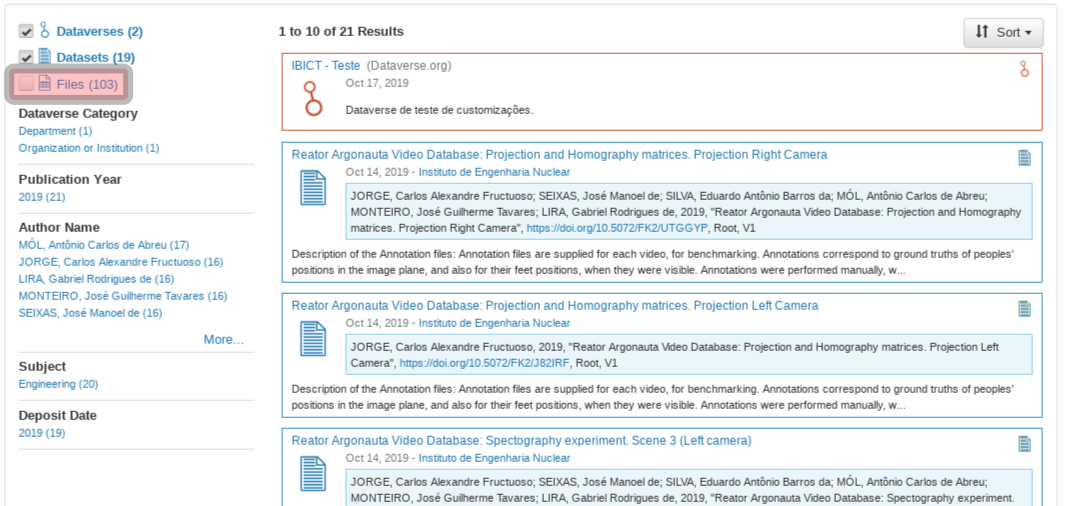
\includegraphics[width=1.0\textwidth]{USAAAA.png}
    \label{print1}
\end{figure}
\noindent  {\small Fonte: Elaboração própria}
   
	    \subsubsection{Citar Dados, versões e metadados}
	   
\qquad Você pode encontrar a citação para o conjunto de dados na parte superior da página do conjunto de dados em uma caixa azul. Além disso, há um botão Citar Dados [3] que oferece a opção de baixar a citação como EndNote XML, RIS Format ou BibTeX Format.
	    
\begin{figure}[H]
\caption{Citar dados}
\centering
    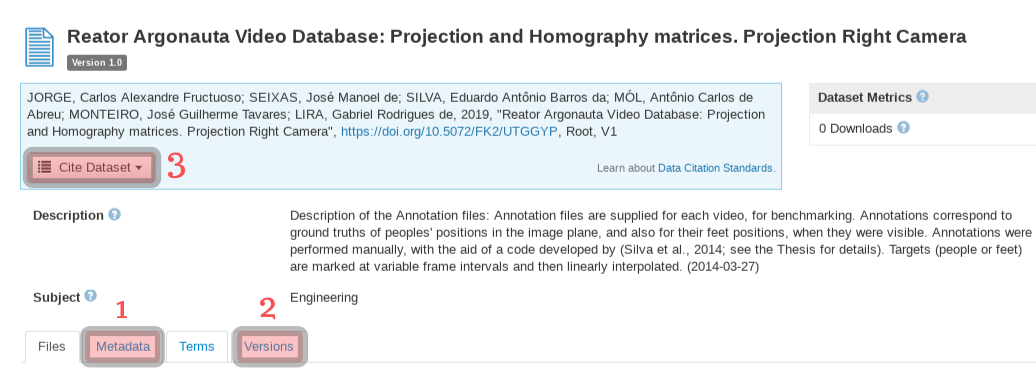
\includegraphics[width=1.0\textwidth]{PFVFU.png}
    \label{print2}
\end{figure}

\noindent  {\small Fonte: Elaboração própria}

    	\subsubsection{Download de arquivos}
    	
\qquad Na guia Arquivos em uma página de conjunto de dados, você pode fazer o download dos arquivos nesse conjunto de dados. Para baixar mais de um arquivo por vez, selecione os arquivos que você deseja baixar e clique no botão Download [1] acima dos arquivos. Os arquivos selecionados serão baixados no formato .zip que preserva qualquer estrutura de pastas que o proprietário do conjunto de dados configurou.

Um arquivo da página do dataset, pode ser baixado, clicando no botão Download [2] no canto superior direito da página ou Fazendo o download via URL na guia Metadados na metade inferior da página.

\begin{figure}[H]
\caption{Arquivos}
\centering
    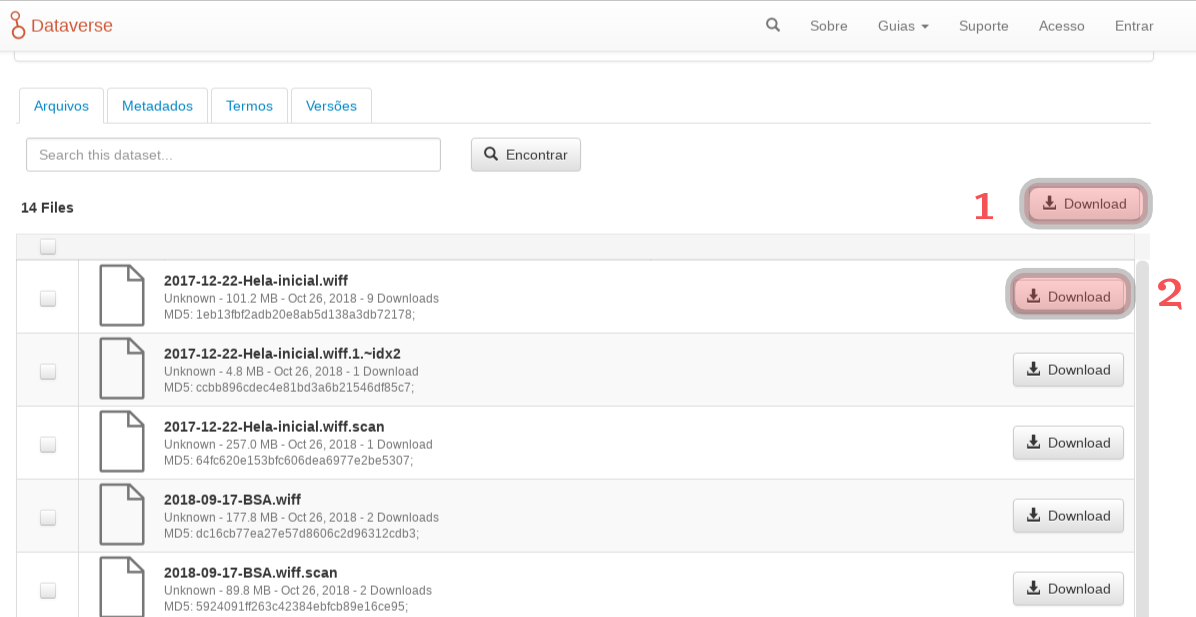
\includegraphics[width=1.0\textwidth]{Prints/p3.png}
    \label{print3}
\end{figure}
\noindent {\small Fonte: Elaboração própria}

    	    \begin{enumerate}[a]
	            \item Dados Tabulares\\
	            
\qquad Os arquivos ingeridos podem ser baixados de várias maneiras diferentes:

\begin{itemize}
\item A opção padrão é baixar um arquivo de valores separados por tabulação, que é um padrão fácil e gratuito de usar;
\item O arquivo original, que pode estar em um formato proprietário, requer software especial;
\item Formato Rdata se a instalação configurou este;
\item Os metadados da variável para o arquivo no formato DDI;
\item Um subconjunto das colunas dos dados.
\end{itemize}
	            
	            \item Downloading via URL
	           
\qquad O Dataverse exibe um URL de texto sem formatação para o local do arquivo na guia Metadados na página do conjunto de dados. Este URL de download pode ser usado para acessar diretamente o arquivo via API (ou em um navegador da Web, se necessário). Ao baixar arquivos maiores, para garantir um download confiável e retomável, recomendamos o uso do GNU Wget em um terminal de linha de comando ou o software gerenciador de download de sua escolha.

\qquad Certos arquivos não fornecem URLs de download por motivos técnicos: aqueles que são restritos, têm termos de uso associados ou fazem parte de um dataverse com um livro de visitas ativado.
	            
	            \item Downloading um pacote Dataverse via URL
	            
\qquad Os pacotes de dataverse são normalmente usados para representar arquivos ou pacotes configuráveis extremamente grandes que contêm um grande número de arquivos. Os pacotes de dataverse geralmente são grandes demais para serem baixados com segurança usando um navegador da web. Quando você clica para baixar um pacote do Dataverse, em vez de iniciar automaticamente o download no navegador da Web, o Dataverse exibe um URL em texto sem formatação para o local do arquivo. Para garantir um download confiável e retomado, recomendamos o uso do GNU Wget em um terminal de linha de comando ou o software gerenciador de download de sua escolha. Se você tentar simplesmente colar o URL no seu navegador da Web, o download poderá sobrecarregá-lo, resultando em um download interrompido, excedido o tempo limite ou com falha.
	            
	        \end{enumerate}
    	\subsubsection{Explore Dados}
	
\qquad Observe que a instalação do Dataverse que você está usando pode ter ferramentas adicionais ou diferentes configuradas como o TwoRavens ou o WorldMap.
	
\newpage

\section{Manual do usuário: Gerenciamento Dataverse}
\vspace{10.5cm}

\qquad Um Dataverse é um contêiner para conjuntos de dados, ou seja: 

\begin{itemize}
    \item dados de pesquisa;
    \item código;
    \item documentação;
    \item metadados;
    \item outros dataverses;
    \item entre outros.
\end{itemize}

Que podem ser configurados para pesquisadores, departamentos, periódicos e organizações individuais.

Depois que um usuário cria um dataverse, por padrão, ele se torna o administrador desse dataverse. O administrador do dataverse tem acesso para gerenciar as configurações.


\begin{figure}[H]
\caption{Diagrama esquemático}
\centering
    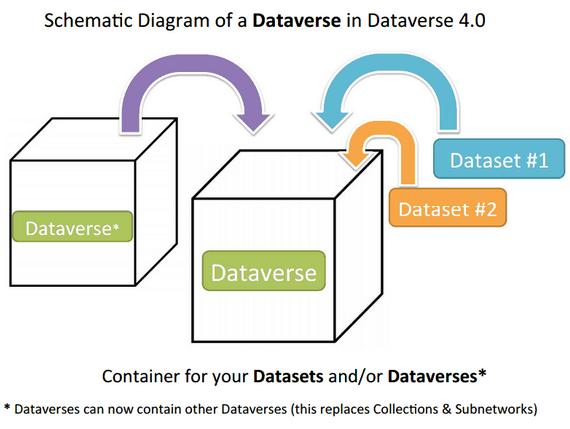
\includegraphics[width=0.8\textwidth]{Dataverse-Diagram.png}
    \label{Diagrama dataverse}
\end{figure}
\noindent {\small Fonte: DATAVERSE PROJECT, 2019}

\subsection{Criação de um Dataverse (Dentro do Dataverse “Root”)}
    
\qquad 1. Para criar um dataverse primeiro você deve ser um usuário registrado. Uma vez logado, clique no botão "Add Data (Adicionar Dados)" e, no menu suspenso, selecione "New Dataverse (Novo Dataverse)".\\

2. Na página "New Dataverse", preencha os seguintes campos:

\begin{itemize}

 \item Nome: digite o nome do seu dataverse.
 \item Identificador: é uma abreviação, geralmente em letras minúsculas, que se torna parte da URL do novo dataverse. Caracteres especiais (\~, `,!, @, \#, \$, \%, \^, \& E *) e espaços não são permitidos. Se você alterar o campo URL do Dataverse, o URL do seu Dataverse será alterado (http //.../ 'url'), e afetará os links para esta página. 
 
 \item E-mail: este é o endereço de e-mail que será usado como contato para esse dataverse específico. Você pode ter mais de um endereço de e-mail de contato para o seu dataverse.
\item Afiliação: adicione qualquer Afiliação que possa ser associada a esse dataverse específico (por exemplo, nome do projeto, nome do instituto, nome do departamento, nome do diário, etc.). Isso é preenchido automaticamente se você adicionou uma afiliação à sua conta de usuário.
\item Descrição: forneça uma descrição desse dataverse. Ela será exibida na página inicial do seu dataverse e na lista de resultados da pesquisa. O campo de descrição suporta determinadas tags HTML.
\item  Categoria: selecione uma categoria que melhor descreva o tipo de dataverse. Por exemplo, se esse é um dataverse para os conjuntos de dados de um pesquisador individual, selecione "Pesquisador". Se for um dataverse para uma instituição, selecione "Organização e instituição".
\item  Escolha os conjuntos de Elementos de metadados para conjuntos de dados neste dataverse: Por padrão, os elementos de metadados serão do dataverse do host em que esse novo dataverse é criado. O Dataverse oferece padrões de metadados para vários domínios.
\item Selecionar facetas para esse dataverse: por padrão, as facetas que aparecerão na sua página de destino do dataverse serão do dataverse host no qual esse novo dataverse foi criado. As facetas são simplesmente campos de metadados que podem ser usados para ajudar outras pessoas a encontrar facilmente dataverses e conjuntos de dados dentro desse dataverse. Você pode selecionar quantas facetas desejar.

 \end{itemize}
 
 \begin{figure}[H]
 \caption{Facetas}
\centering
    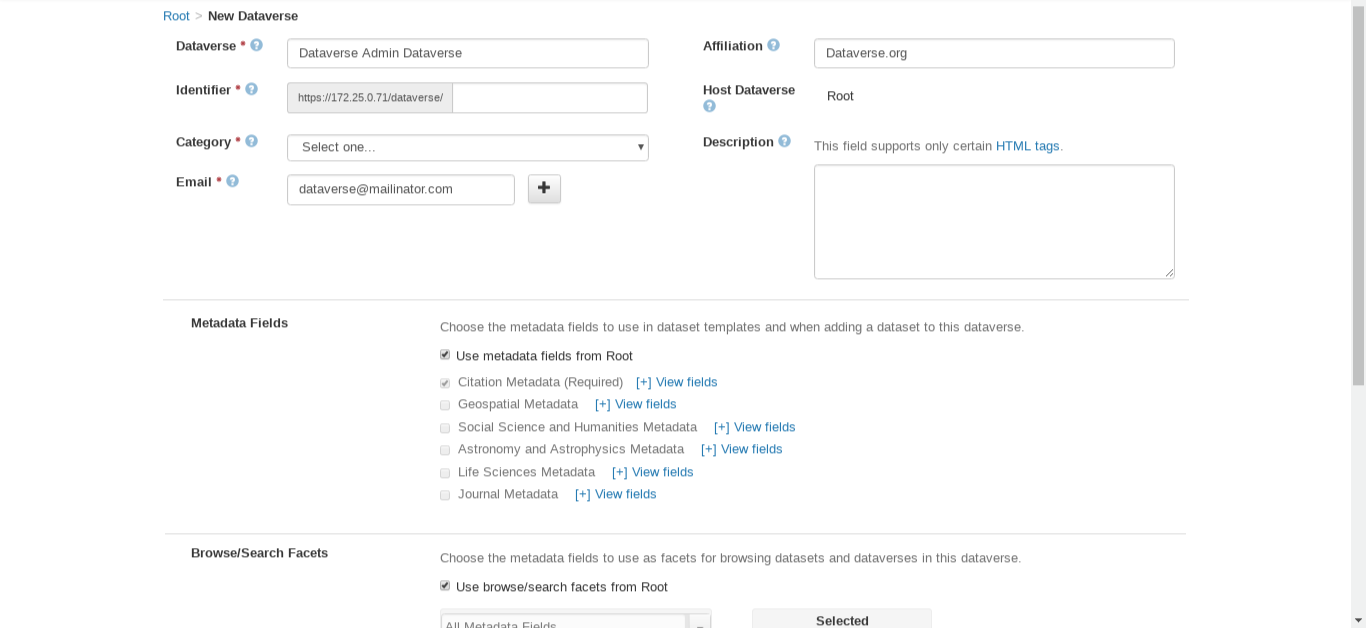
\includegraphics[width=1.0\textwidth]{Prints/p4.png}
    \label{print4}
\end{figure}
\noindent {\small Fonte: Elaboração própria}\\
 
3. Os elementos de metadados selecionados também são usados para escolher quais campos de metadados você gostaria de usar para criar modelos para seus conjuntos de dados. Os campos de metadados podem ser ocultos ou selecionados conforme necessário ou opcional. Depois de selecionar todos os campos que gostaria de usar, você poderá criar seu (s) modelo (s) depois de terminar de criar seu dataverse.\\

4. Clique no botão "Create Dataverse (Criar Dataverse)"\\

Os campos obrigatórios são indicados por um asterisco vermelho.
    
    \subsection{Edite um Dataverse}
    
\qquad Para editar seu dataverse, navegue até a página inicial do dataverse e selecione o botão "Edit Dataverse (Editar dataverse)", onde serão apresentadas as seguintes opções de edição:

\begin{itemize}

    \item Informações gerais: editar nome, identificador, categoria, e-mail de contato, afiliação, descrição, elementos de metadados e facetas para o seu dataverse;
    \item Tema: faça upload de um logotipo para o seu dataverse, adicione um link ao seu departamento ou site pessoal e selecione cores para o dataverse para marcá-lo;
    \item Widgets: obtenha um código para adicionar ao seu site e exibir seu dataverse nele;
    \item Permissões: conceda aos usuários do Dataverse permissões para o seu dataverse, ou seja, pode editar conjuntos de dados e ver quais usuários já possuem quais permissões para quais dataverse;
    \item Modelos de conjunto de dados: são úteis quando você tem vários conjuntos de dados com as mesmas informações em vários campos de metadados que você não precisará digitar manualmente toda vez;
    \item Livros de visitas do conjunto de dados: permite coletar dados sobre quem está baixando os arquivos dos seus conjuntos de dados;
    \item Dataverses em destaque: se você tiver um ou mais dataverses, poderá usar esta opção para mostrá-los na parte superior da página do dataverse para ajudar outras pessoas a encontrar facilmente dataverses interessantes ou importantes;
    \item Excluir o Dataverse: você pode excluir o seu dataverse desde que não seja publicado e não possua nenhum rascunho de conjuntos de dados.
    
\end{itemize}

    \subsection{Informação geral}
    
\qquad A página "Informações gerais" é como você edita as informações preenchidas enquanto cria seu dataverse. Se você precisar alterar ou adicionar um endereço de e-mail de contato, este é o local para fazê-lo. Além disso, você pode atualizar os elementos de metadados usados para conjuntos de dados no dataverse, alterar quais campos de metadados estão ocultos, necessários ou opcionais e atualizar as facetas que você gostaria que fossem exibidas para navegar no dataverse. Se você planeja usar modelos, será necessário selecionar os campos de metadados na página Informações gerais.

Os campos de metadados que você selecionar conforme necessário aparecerão no formulário Criar conjunto de dados quando alguém adicionar um conjunto de dados ao dataverse.

 \begin{figure}[H]
 \caption{Campos}
\centering
    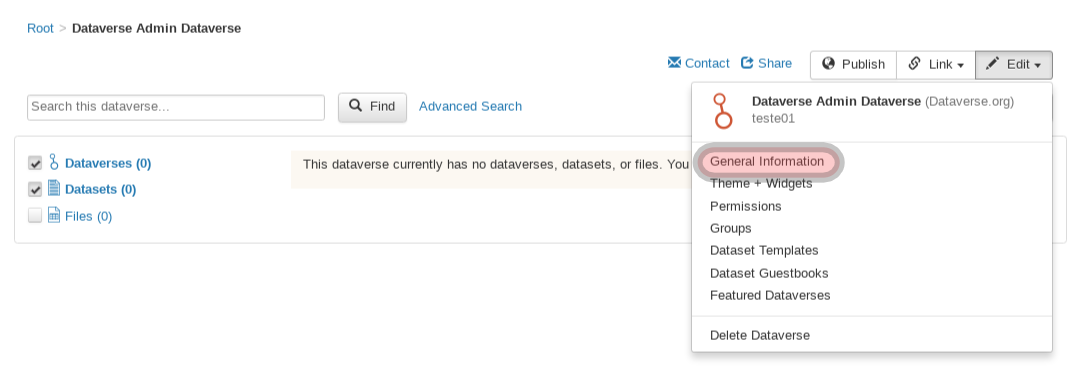
\includegraphics[width=1.0\textwidth]{Prints/p5.png}
    \label{print5}
\end{figure}
\noindent {\small Fonte: Elaboração própria}

    \subsection{Tema}
    
\qquad O recurso Tema fornece uma maneira de personalizar a aparência do seu dataverse. Você pode optar por usar o tema do dataverse que contém o dataverse (até o dataverse raiz, também conhecido como a página inicial) ou fazer upload de seu próprio arquivo de imagem. Os tipos de imagem suportados são JPEG, TIFF ou PNG e não devem ter mais que 500 KB. O tamanho máximo de exibição de um arquivo de imagem no tema de um dataverse é de 940 pixels de largura por 120 pixels de altura. As cores para o cabeçalho do seu dataverse e o texto que aparece no dataverse também podem ser selecionadas. Um link também pode ser adicionado ao seu site pessoal, o site da sua organização ou instituição, seu departamento, diário, etc.

    \subsection{Widgets}
    
\qquad O recurso Widgets fornece código para você colocar em seu site pessoal e exibir seu dataverse lá. Existem dois tipos de Widgets para um dataverse, um widget Caixa de Pesquisa do Dataverse e um widget da Listagem do Dataverse. Na guia Widgets da página Tema + Widgets, você pode copiar e colar os trechos de código do widget que você deseja adicionar ao seu site. Se você precisar ajustar a altura do widget em seu site, poderá fazê-lo editando o parâmetro heightPx = 500 no snippet de código.
    
        \subsubsection{Widget Caixa de Pesquisa}
    
\qquad O Widget da Caixa de Pesquisa do Dataverse adicionará uma caixa de pesquisa ao seu site vinculada ao seu dataverse. Os usuários são direcionados ao seu dataverse em uma nova janela do navegador para exibir os resultados dos termos de pesquisa inseridos no campo de entrada.
    
        \subsubsection{Widget Lista}

\qquad O widget de listagem de dados dataverses fornece uma lista de todos os seus dataverses e conjuntos de dados para os usuários procurarem, classificarem, filtrarem e pesquisarem. Quando alguém clica em um dataverse ou conjunto de dados no widget, ele exibe o conteúdo no widget no seu site. Eles podem baixar arquivos de dados diretamente dos conjuntos de dados no widget. Se um arquivo for restrito, eles serão direcionados ao seu dataverse para efetuar login, em vez de fazer o login através do widget em seu site.
    
    \subsection{Papéis e Permissões}
    
\qquad As contas de usuário do dataverse podem receber funções que definem quais ações têm permissão para executar em dataverses, conjuntos de dados e / ou arquivos específicos. Cada função vem com um conjunto de permissões, que definem as ações específicas que os usuários podem executar.

Funções e permissões também podem ser concedidas a grupos. Grupos podem ser definidos como uma coleção de contas de usuário do Dataverse, uma coleção de endereços IP (por exemplo, todos os usuários dos computadores de uma biblioteca) ou uma coleção de todos os usuários que efetuam login usando um login institucional específico (por exemplo, todos que efetuam login com um determinado credenciais de conta da universidade).

Os administradores de um dataverse podem atribuir funções e permissões aos usuários desse dataverse. Se você é um administrador em um dataverse, encontrará o link para a página "Permissões", no menu suspenso Editar, na página do dataverse.

\newpage

\begin{figure}[H]
\caption{Permissões}
\centering
    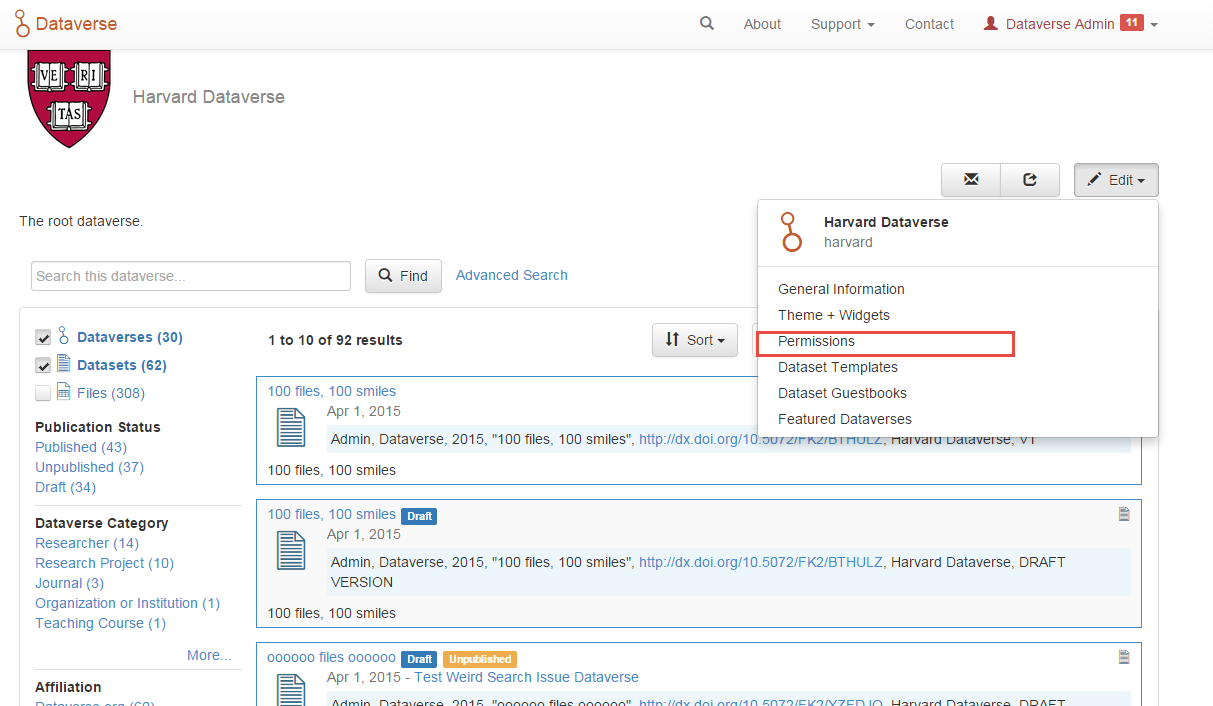
\includegraphics[width=1.0\textwidth]{prt1.png}
    
    \label{Permissões}
\end{figure}
\noindent {\small Fonte: DATAVERSE PROJECT, 2019}

\begin{figure}[H]
\caption{Página permissões}
\centering
    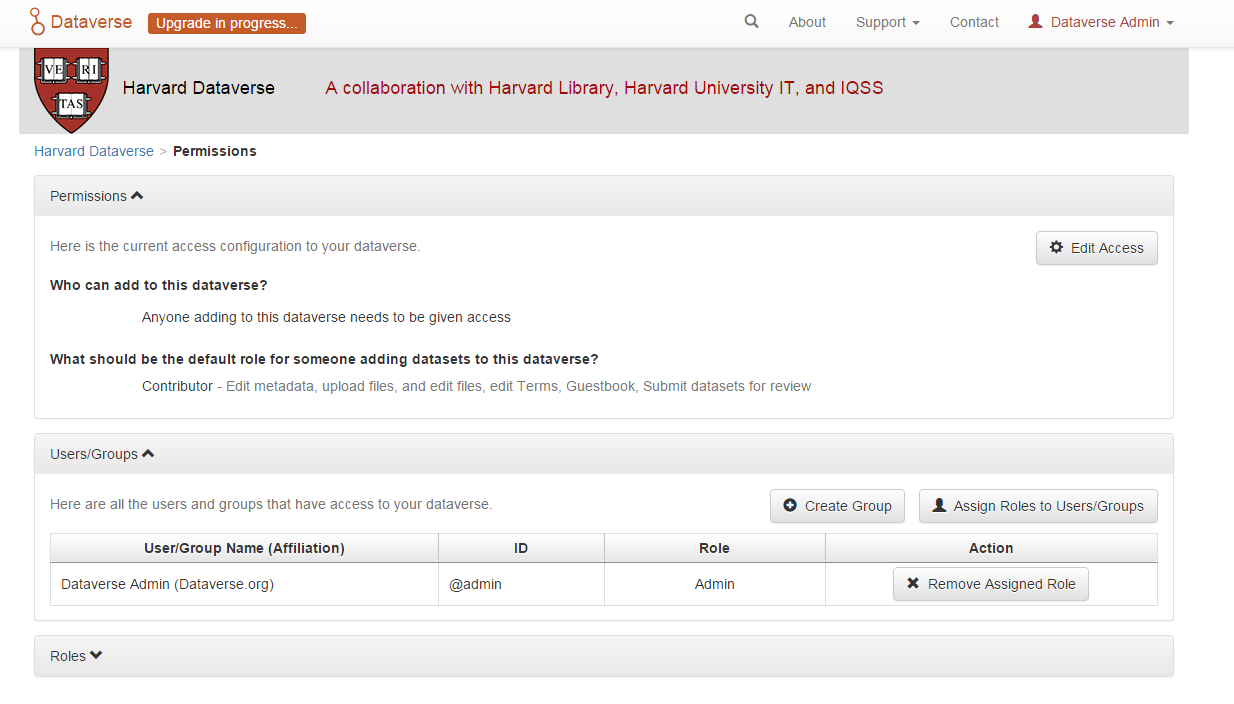
\includegraphics[width=1.0\textwidth]{NOVOTIR.png}
    \label{Permissões 2}
\end{figure}
\noindent {\small Fonte: DATAVERSE PROJECT, 2019}\\

Ao acessar a página de permissões de um dataverse, você visualizará três seções:\\

\textbf{Permissões:} Define os requisitos que determinam quais tipos de usuários podem adicionar conjuntos de dados e subavaliadores de dados ao seu dataverse e quais permissões serão concedidas quando o fizerem.\\

\textbf{Usuários / Grupos:} Atribui funções a usuários ou grupos específicos, determinando quais ações eles têm permissão para executar no seu dataverse. Poderá também pode fazer referência a uma lista de todos os usuários que têm funções atribuídas a eles para o seu dataverse e remover as funções, se desejar.\\

\textbf{Funções:} Elabora uma lista completa de funções que podem ser atribuídas aos usuários do seu dataverse. Cada função lista as permissões que oferece. Observe que, mesmo em um dataverse recém-criado, você poderá ver que usuários e grupos já receberam funções, se sua instalação tiver: Conjunto de InheritParentRoleAssignments.

        \subsubsection{Definindo Configurações de Acesso}
        
\qquad Na guia Permissões, você pode clicar no botão "Edit Access (Editar acesso)" para abrir uma caixa onde você pode definir quem irá adicionar itens ao seu dataverse e quais permissões são concedidas àqueles que os adicionam.
        
  \begin{figure}[H]
  \caption{Tipos de permissão}
         \centering
    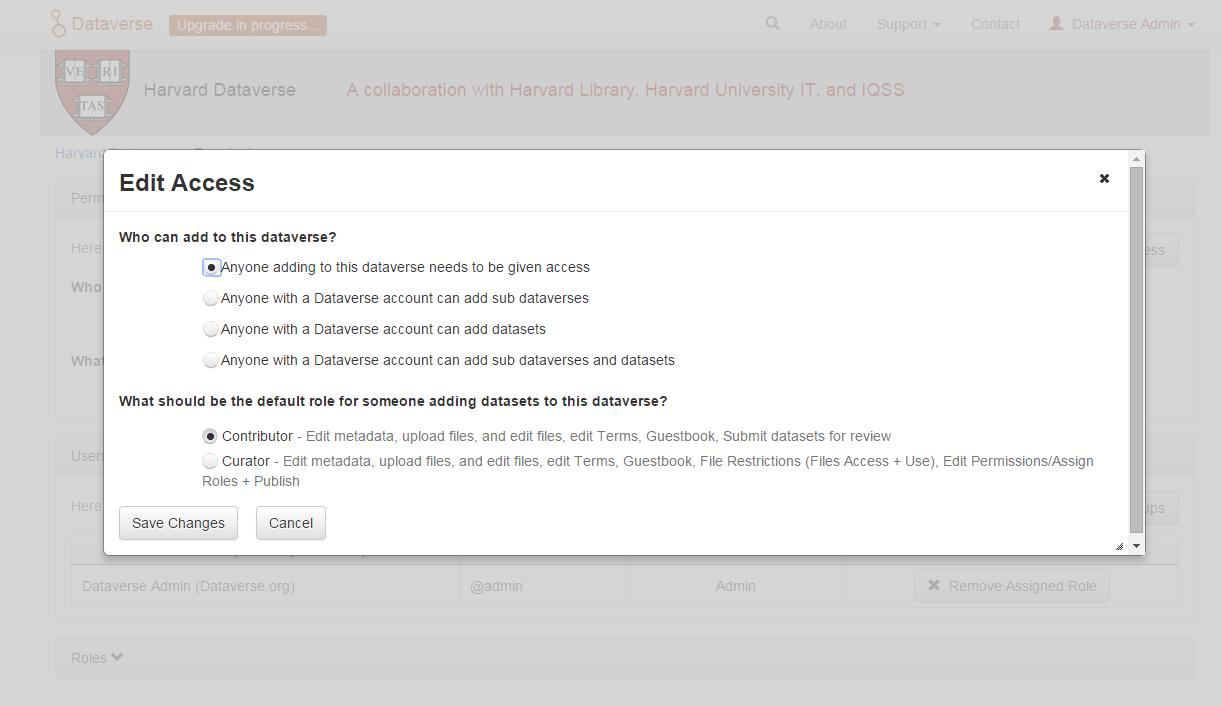
\includegraphics[scale=0.4]{prt3.png}
    \label{Acesso}
    \end{figure}
  \noindent {\small Fonte: DATAVERSE PROJECT, 2019}\\
  
 A primeira pergunta nesta página permite determinar como é aberto o seu dataverse para novas adições - você pode definir se a base de usuários inteira (todos os usuários logados) tem ou não a capacidade de adicionar conjuntos de dados ou sub-dataverses ao seu dataverse.

A segunda pergunta nesta página permite escolher a função (e, portanto, as permissões) concedidas aos usuários que adicionam um conjunto de dados ao seu dataverse. A função que você selecionar será concedida automaticamente a qualquer usuário que criar um conjunto de dados no seu dataverse, nesse conjunto de dados, no momento em que o criar. A função que o usuário recebe determina suas permissões para o conjunto de dados que ele criou. A principal diferença entre as duas funções é que os curadores podem publicar seus próprios conjuntos de dados, enquanto os colaboradores devem enviar o conjunto de dados para revisão antes da publicação. Além disso, os curadores podem gerenciar as permissões do conjunto de dados. Observe que essa configuração não aplica funções retroativamente aos usuários que adicionaram conjuntos de dados anteriormente ao seu dataverse; aplica-se apenas aos usuários que adicionam novos conjuntos de dados daqui para frente. Ambas as configurações podem ser alteradas a qualquer momento.
        
        \subsubsection{Definindo papéis para Usuários e Grupos}
        
\qquad Na guia Usuários / Grupos, você pode adicionar, editar ou remover as funções concedidas a usuários e grupos no seu dataverse. Uma função é um conjunto de permissões concedidas a um usuário ou grupo que estiver usando seu dataverse. Por exemplo, atribuir ao seu assistente de pesquisa a função "Colaborador" lhe daria as seguintes permissões autoexplicativas no seu dataverse e em todos os conjuntos de dados dentro do dataverser: "ViewUnpublishedDataset", "DownloadFile", "EditDataset" e "DeleteDatasetDraft". 

Essa função, no entanto, não teria a permissão "PublishDataset" e, portanto, seria incapaz de publicar conjuntos de dados no seu dataverse. Se você quisesse dar a ela essa permissão, você daria a ela um papel com essa permissão, como por exemplo o papel de Curador. Usuários e grupos podem ter várias funções ao mesmo tempo, se necessário. As funções podem ser removidas a qualquer momento. Todas as funções e suas permissões associadas são listadas na guia "Funções" da mesma página.
        
\begin{figure}[H]
  \caption{Papéis}
        \centering
     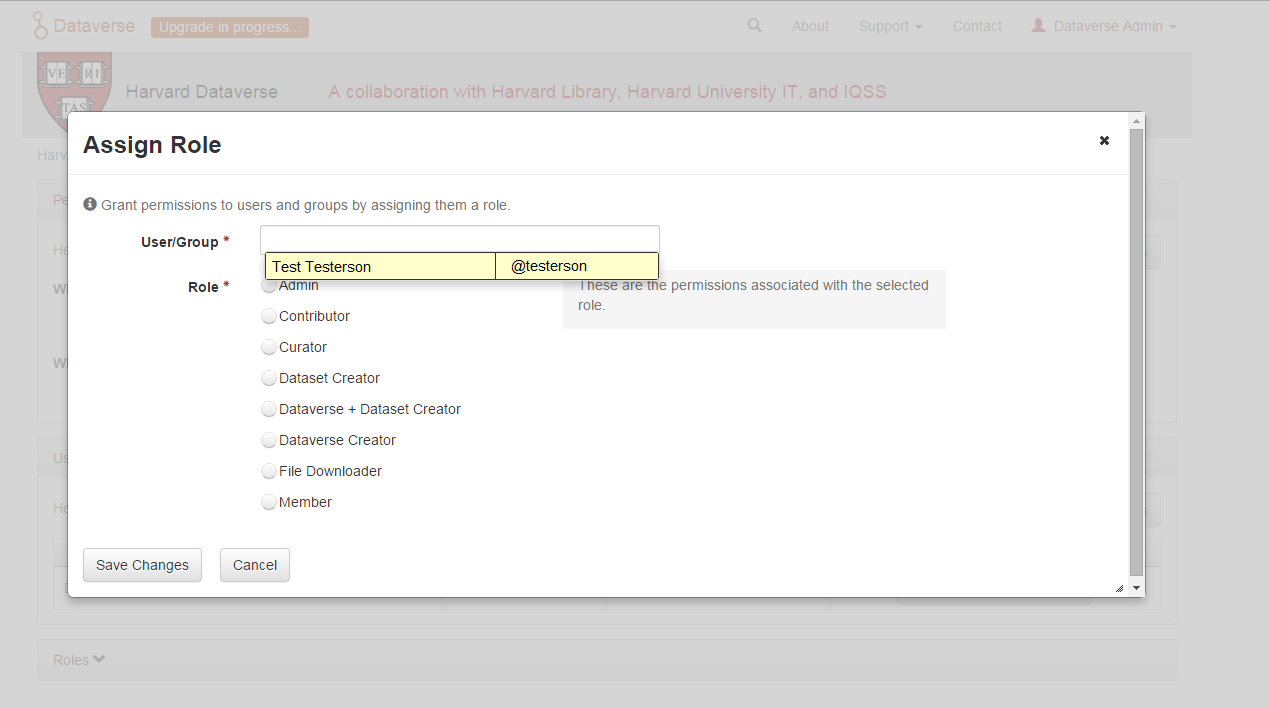
\includegraphics[scale=0.4]{prt4.png}
            \label{Acesso 2}
        \end{figure}
\noindent {\small Fonte: DATAVERSE PROJECT, 2019}\\
        
Observe que a função Criador do conjunto de dados e a função Colaborador às vezes são confusas. A função Criador do conjunto de dados é atribuída no nível do dataverse e permite que um usuário crie novos conjuntos de dados nesse dataverse. A função Colaborador pode ser atribuída no nível do conjunto de dados, concedendo ao usuário a capacidade de editar esse conjunto de dados específico. Como alternativa, a função Colaborador pode ser atribuída no nível do dataverse, concedendo ao usuário a capacidade de editar todos os conjuntos de dados nesse dataverse.

\begin{figure}[H]
 \caption{Designando papéis}
                \centering           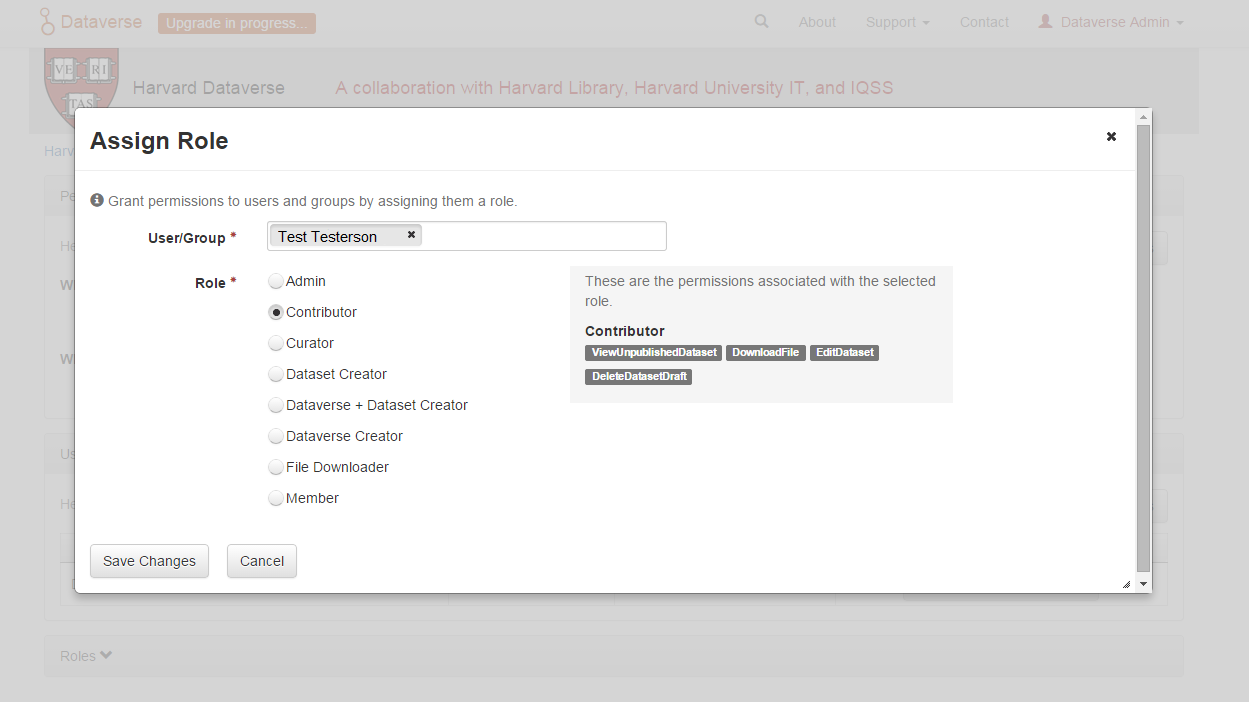
\includegraphics[scale=0.4]{prt5.png}
            \label{Acesso 3}
        \end{figure}
\noindent {\small Fonte: DATAVERSE PROJECT, 2019}\\

Se você precisar atribuir uma função a TODAS as contas de usuário do Dataverse, poderá atribuir a função ao grupo: "usuários autenticados”.
        
    \subsection{Templates de Dataset}
    
\qquad Os modelos são úteis quando você tem vários conjuntos de dados com as mesmas informações em vários campos de metadados que você prefere não continuar digitando manualmente ou se deseja usar um conjunto personalizado de "Termos de Uso e Acesso" para vários conjuntos de dados em um dataverse. 

No Dataverse, os modelos são criados no nível do dataverse, podem ser excluídos (para que não sejam exibidos para futuros conjuntos de dados), definidos como padrão (não obrigatório) ou podem ser copiados para que você não precise recomeçar ao criar um novo modelo com metadados semelhantes de outro modelo. Quando um modelo é excluído, ele não afeta os conjuntos de dados que já o usaram, ou seja, os conjuntos de dados que já utilizam um modelo não terão seu modelo trocado ou excluído.\\

 \begin{figure}[H]
  \caption{Termos de uso}
\centering
    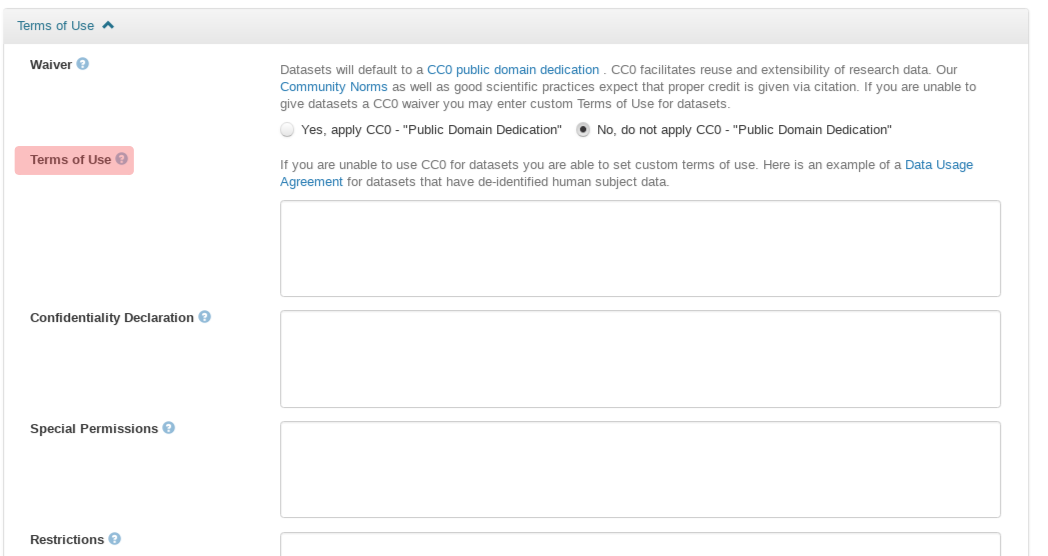
\includegraphics[width=1.0\textwidth]{Prints/pn1.png}
    \label{print6}
\end{figure}
\noindent {\small Fonte: Elaboração própria}\\

Para criar um modelo:\\

\qquad 1. Navegue para o seu daverse, clique no botão Editar dataverso e selecione Modelos de conjunto de dados.\\

 \begin{figure}[H]
 \caption{Livros de visita}
\centering
    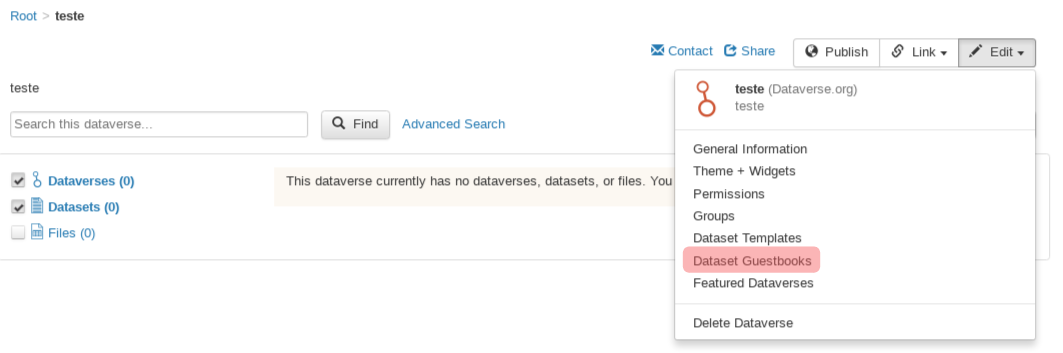
\includegraphics[width=1.0\textwidth]{Prints/pn2.png}
    \label{print7}
\end{figure}
\noindent {\small Fonte: Elaboração própria}\\

\qquad 2. Depois de clicar em Modelos de conjunto de dados, você será levado à página Modelos de conjunto de dados. Nesta página, você pode primeiro decidir usar os modelos de conjunto de dados do seu dataverse pai depois criar um novo modelo de conjunto de dados ou fazer as duas coisas.\\

\qquad 3. Clique no Criar modelo de conjunto de dados para começar. Você verá que o modelo é igual à página de criação de conjunto de dados com um campo adicional na parte superior da página para adicionar um nome ao modelo.\\

\qquad 4. Depois de adicionar informações aos campos de metadados para as quais você tem informações e clicar em Salvar e adicionar termos, você será levado à página onde poderá adicionar Termos de uso e acesso personalizados. Se você não precisar de Termos de uso e acesso personalizados, clique no modelo Salvar conjunto de dados e apenas os campos de metadados serão salvos.\\

\qquad 5. Depois de clicar em Salvar modelo de conjunto de dados, você será levado de volta à página Gerenciar modelos de conjunto de dados e visalizará seu modelo listado agora com as opções de predefinição, edição, exibição ou exclusão.\\

\qquad 6. Um dataverse não precisa ter um modelo padrão e os usuários podem selecionar qual modelo eles gostariam de usar na página Criar conjunto de dados.\\

\qquad 7. No botão Exibir na página "Gerenciar modelos de conjunto de dados", será possível visualizar quais campos de metadados têm informações preenchidas. Observe que a capacidade de escolher quais campos de metadados estão ocultos, obrigatórios ou opcionais é feita na página Informações gerais do dataverse.
    
    \subsection{Livro de visitas de Datasets}
    
\qquad Os livros de visitas permitem coletar dados sobre quem está baixando os arquivos dos seus conjuntos de dados. Você pode decidir coletar informações da conta (nome de usuário, nome e sobrenome, afiliação, etc.), além de criar perguntas personalizadas (por exemplo, para o que planeja usar esses dados?). Você também pode fazer o download dos dados coletados dos livros de visitas ativados como arquivos do Excel para armazenar e usar fora do Dataverse.\\

Para criar um livro de visitas:\\

\qquad 1. Depois de criar um dataverse, clique no botão Editar dataverse e selecione Conjunto de dados do livro de visitas\\

\qquad 2. Por padrão, os livros de visitas criados no dataverse em que o dataverse está, serão exibidos. Se você não quiser usar ou ver esses livros de visitas, desmarque a caixa de seleção: Incluir Livros de Visitas do Root Dataverse.\\

\qquad 3. Para criar um novo livro de visitas, clique no botão Criar livro de visitas do conjunto de dados no lado direito da página.\\

\qquad 4. Nomeie o livro de visitas, determine as informações da conta que você gostaria que fossem solicitadas (todos os campos de informações da conta aparecem quando alguém baixa um arquivo) e adicione Perguntas personalizadas (podem ser necessárias ou não).\\

\qquad 5. Clique no botão Criar livro de visitas do conjunto de dados depois de terminar.\\

Depois de criar um livro de visitas, observará que existem várias opções para um livro de visitas e aparecerá na lista de livros de visitas.

Se você deseja usar um livro de visitas que criou, primeiro clique no botão no menu ativo que diz Ativar. Depois que um livro de visitas for ativado, você poderá acessar os Termos de Licença + para um conjunto de dados e selecionar um livro de visitas para ele.
Também há opções para visualizar, copiar, editar ou excluir um livro de visitas.
Depois que alguém fizer o download de um arquivo em um conjunto de dados em que um livro de visitas foi atribuído, uma opção para baixar os dados coletados será exibida.
    
    \subsection{Dataverses destaques}
    
\qquad Os Dataverses em destaque são uma maneira de exibir sub-dataverses no seu dataverse que você deseja destacar para que as pessoas vejam facilmente quando o visitam.

Clique em Dataverses em destaque e um pop-up aparecerá. Selecione quais sub-dataverses você gostaria que fossem exibidos. Dataverses em destaque podem ser usados apenas com dataverses publicados.
    
    \subsection{Vinculação de Datasets}
    
\qquad A vinculação de conjunto de dados permite que um proprietário do dataverse "vincule" seu dataverse a um conjunto de dados que exista fora desse dataverse, para que apareça na lista de conteúdos do dataverse sem realmente estar nesse dataverse. Você pode vincular os conjuntos de dados de outros usuários ao seu dataverse, mas isso não transfere a edição ou outras permissões especiais para você. O conjunto de dados vinculado ainda estará sob o controle do usuário original.

Por exemplo, os pesquisadores que trabalham em um estudo colaborativo entre instituições podem cada um vincular seus próprios dados institucionais individuais ao conjunto de dados colaborativo, facilitando a localização do estudo pelas partes interessadas de cada instituição.

Para vincular um conjunto de dados, você precisará da sua conta com a permissão "Adicionar conjunto de dados" no Dataverse que está fazendo o link. Se você criou o dataverse, já deve ter essa permissão, mas, caso contrário, precisará solicitar ao administrador desse dataverse que atribua essa permissão à sua conta. Você não precisa de permissões especiais no conjunto de dados que está sendo vinculado.

Para vincular um conjunto de dados ao seu dataverse, você deve navegar até esse conjunto de dados e clicar no botão branco "Link" no canto superior direito da página do conjunto de dados. Isso abrirá uma janela na qual você pode digitar o nome do dataverse que deseje vincular o conjunto de dados. Selecione seu dataverse e clique no botão Salvar. Isso estabelecerá o link, e o conjunto de dados aparecerá agora no seu dataverse. Atualmente, não há como remover links estabelecidos na interface do usuário.
    
    \subsection{Vinculação de Dataverses}
    
\qquad A vinculação de conjunto de dados permite que um proprietário do dataverse "vincule" seu dataverse a um conjunto de dados que exista fora desse dataverse, para que ele apareça na lista de conteúdos do dataverse sem realmente estar nesse dataverse. Você pode vincular os conjuntos de dados de outros usuários ao seu dataverse, mas isso não transfere a edição ou outras permissões especiais para você. O conjunto de dados vinculado ainda estará sob o controle do usuário original.

Da mesma forma que a vinculação de conjuntos de dados, a vinculação de dataverses permite que um proprietário de um dataverse "vincule" seu dataverse a outro dataverse, para que o dataverse que está sendo vinculado apareça na lista de conteúdos do vinculador de dados sem realmente estar nesse dataverse. Atualmente, a capacidade de vincular um dataverse a outro dataverse é um recurso exclusivo do superusuário.

    \subsection{Publique seu Dataverse}
    
\qquad Quando o seu dataverse estiver pronto para ir a público, vá para a sua página, clique no botão "Publicar" no lado direito da página. Um pop-up aparecerá para confirmar que você está realmente pronto para publicar, uma vez que um dataverse é tornado público, esta ação não pode mais ser desfeita.

\newpage

\section{Manual do usuário: Dataset + Gerenciamento de arquivos}
\vspace{10.0cm}

\qquad Um conjunto de dados no Dataverse é um contêiner para seus dados, documentação, código e os metadados que descrevem esse conjunto de dados.

\begin{figure}[H]
 \caption{Esquema de um Dataset}
                \centering
             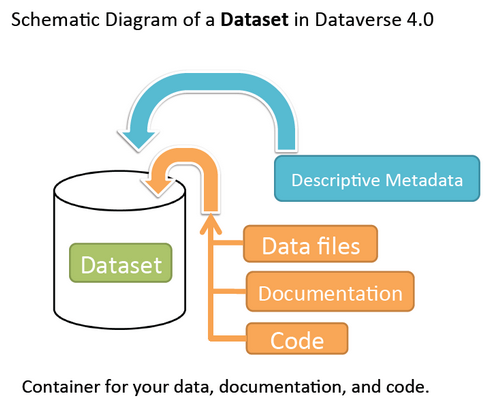
\includegraphics[scale=0.5]{dtset.png}
            \label{Dataset}
        \end{figure}
\noindent {\small Fonte: DATAVERSE PROJECT, 2019}

    \subsection{Metadata suportados}
    
\qquad Um conjunto de dados contém três níveis de metadados:\\

\textbf{1. Metadados de citação:} qualquer metadado necessário para gerar uma citação de dados e outros metadados gerais que possam ser aplicados a qualquer conjunto de dados;\\

\textbf{2. Metadados específicos de domínio:} atualmente, com suporte específico para conjuntos de dados de Ciências Sociais, Ciências da Vida, Geoespaciais e Astronomia; e\\

\textbf{3. Metadados no nível do arquivo:} varia de acordo com o tipo de arquivo de dados.

    
        \subsubsection{Formatos de exportação de metadados}
        
\qquad Depois que um conjunto de dados é publicado, seus metadados são exportados em vários formatos. Um botão na guia de metadados da página do conjunto de dados permitirá que um usuário exporte os metadados da versão publicada mais recente do conjunto de dados. Os formatos de exportação atualmente suportados são:

\begin{itemize}

 \item Dublin Core
 \item DDI (Iniciativa de Documentação de Dados)
 \item DataCite 4
 \item JSON (formato nativo do Dataverse)
 \item OAI\_ORE
 \item OpenAIRE

\end{itemize}
        
    \subsection{Adicionando um novo Dataset}
    
\qquad 1. Navegue para o dataverse no qual você deseja adicionar um conjunto de dados.\\

2. Clique no botão "Add Data (Adicionar dados)" e selecione "New Dataset (Novo conjunto de dados)" no menu suspenso.\\

3. Para começar rapidamente, insira no mínimo todos os campos obrigatórios com um asterisco (por exemplo, título do conjunto de dados, autor, descrição, e-mail de contato e assunto) para obter uma citação de dados com um DOI.\\

4. Role para baixo até a seção "Arquivos", e clique em "Select Files to Add (Selecionar arquivos a serem adicionados)" para adicionar todos os arquivos relevantes ao seu conjunto de dados. Você também pode enviar seus arquivos diretamente do seu Dropbox. Você pode arrastar e soltar ou selecionar vários arquivos de uma vez da área de trabalho diretamente no widget de upload. Seus arquivos aparecerão abaixo do botão "Select Files to Add (Selecionar arquivos a serem adicionados)", onde você pode adicionar uma descrição e tags (através do botão " Edit tag (Editar tag)") para cada arquivo. Além disso, uma soma de verificação MD5 será adicionada para cada arquivo. Se você enviar um arquivo tabular, uma Impressão Digital Numérica Universal (UNF) será adicionada a esse arquivo.\\

5. Clique no botão "Save Dataset (Salvar conjunto de dados)" quando terminar. Seu conjunto de dados não publicado será criado.\\

Você pode adicionar metadados adicionais depois de concluir a criação do conjunto de dados inicial, indo em Editar conjunto de dados> Metadados.

    
    \subsection{Upload de Arquivo}
    
\qquad O software Dataverse oferece vários métodos de upload de arquivos para um conjunto de dados. Esses métodos de upload são configuráveis pelo administrador de uma instalação do Dataverse, portanto, talvez você não veja algumas dessas opções no site do Dataverse que está usando.

Se houver várias opções de upload disponíveis, você deverá escolher qual delas usar para o seu conjunto de dados. Um conjunto de dados pode usar apenas um método de upload. Depois de fazer o upload de um arquivo usando um dos métodos de upload disponíveis, esse método é bloqueado para esse conjunto de dados. Se você precisar mudar os métodos de upload para um conjunto de dados que já contém arquivos, entre em contato com o Suporte clicando no link Suporte, na parte superior do aplicativo.

Você pode fazer upload de arquivos para um conjunto de dados enquanto cria esse conjunto de dados. Você também pode fazer upload de arquivos depois de criar um conjunto de dados, clicando no botão "Edit (Editar)" na parte superior da página do conjunto de dados e na lista suspensa selecionando "Arquivos (Upload)" ou clicando no botão "Upload files) Upload de arquivos" acima da tabela de arquivos em Arquivos aba. Em qualquer uma das opções, você será direcionado para a página Carregar arquivos para esse conjunto de dados.

Certos tipos de arquivo no Dataverse são suportados por funcionalidades adicionais, que podem incluir o download em diferentes formatos, subconjuntos, preservação de metadados no nível do arquivo, citação de dados no nível do arquivo, e exploração através da visualização e análise de dados.
    
    \subsection{Manuseio de Arquivo}
    
\qquad Certos tipos de arquivo no Dataverse são suportados por funcionalidades adicionais, que podem incluir o download em diferentes formatos, subconjuntos, preservação de metadados no nível do arquivo, citação de dados no nível do arquivo; e exploração através da visualização e análise de dados. Consulte as seções abaixo para obter informações sobre funcionalidades especiais para tipos de arquivos específicos.

    \subsection{Arquivos de dados tabulares}
    
\qquad Arquivos em determinados formatos - Stata, SPSS, R, Excel (xlsx) e CSV - podem ser ingeridos como dados tabulares. Os arquivos de dados tabulares podem ser mais explorados e manipulados.

Opções de download adicionais disponíveis para dados tabulares (encontradas no mesmo menu suspenso no botão "Download"):

\begin{itemize}

   \item Como dados delimitados por tabulação (com os nomes das variáveis na primeira linha);
   \item O arquivo original carregado pelo usuário;
   \item Salvo como dados R (se o arquivo original não estava no formato R);
   \item Metadados variáveis (como um arquivo XML do DDI Codebook);
   \item Citação de arquivo de dados (atualmente no formato RIS, EndNote XML ou BibTeX);
   \item Tudo acima, como um pacote compactado.

\end{itemize}
    
\begin{figure}[H]
\caption{Download}
                \centering
             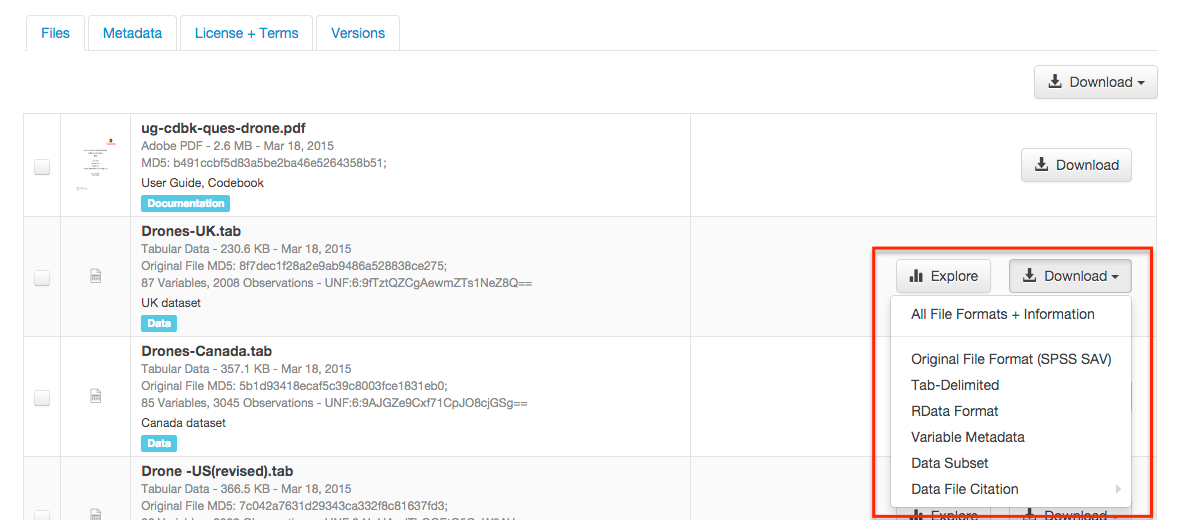
\includegraphics[scale=0.3]{dttab.png}
            \label{Tabulares}
        \end{figure}
    \noindent {\small Fonte: DATAVERSE PROJECT, 2019}
    
    \subsection{Arquivos compactados}
    
\qquad Os arquivos compactados no formato .zip são descompactados automaticamente. Se um arquivo .zip falhar ao descompactar por qualquer motivo, ele será carregado como está. Se o número de arquivos internos for superior a um limite definido (1.000 por padrão, configurável pelo administrador), você receberá uma mensagem de erro e o arquivo .zip será carregado como está.

Se o arquivo .zip carregado contiver uma estrutura de pastas, o Dataverse acompanhará essa estrutura. A localização de um arquivo nessa estrutura de pastas é exibida nos metadados do arquivo como o Caminho do arquivo. Quando você baixa o conteúdo do conjunto de dados, essa estrutura de pastas é preservada e os arquivos aparecem em seus locais originais.

Esses nomes de pasta estão sujeitos a regras estritas de validação. Somente os seguintes caracteres são permitidos: alfanuméricos, '\_', '-', '.' E '(espaço em branco). Quando um arquivo zip é carregado, os nomes das pastas são limpos automaticamente, com os caracteres inválidos substituídos pelo caractere '.' Quaisquer sequências de pontos são substituídas por um único ponto. Por exemplo, o nome da pasta data \& info / code = \@ 137 será convertido em data.info/code.137. Ao fazer o upload pela interface da Web, o usuário pode alterar ainda mais os valores no formulário de edição apresentado antes de clicar no botão "Save (Salvar)".

Se você carregar vários arquivos .zip em um conjunto de dados, todos os subdiretórios idênticos entre vários .zips serão mesclados quando o usuário fizer o download do conjunto de dados completo.
    
    \subsection{Outros tipos de arquivo}
    
\qquad Existem várias opções avançadas disponíveis para determinados tipos de arquivo. Arquivos de imagem: arquivos .jpg, .png e .tif podem ser selecionados como miniatura padrão de um conjunto de dados. A miniatura selecionada aparecerá no cartão de resultados da pesquisa para esse conjunto de dados.
Arquivos SPSS: os arquivos SPSS podem ser marcados com o idioma em que foram originalmente codificados. Isso pode ser encontrado clicando em Opções avançadas e selecionando o idioma na lista fornecida.    
    
    \subsection{Editar Arquivos}

        \subsubsection{Editar Arquivo de Metadados}
        
\qquad Vá para o conjunto de dados que você deseja editar, onde verá a lista de arquivos. Selecione os arquivos que você deseja editar usando a caixa de seleção Selecionar tudo ou selecionando arquivos individualmente. Em seguida, clique no botão "Edit files (Editar arquivos)" acima da tabela de arquivos e, no menu suspenso, selecione se você deseja:

\begin{itemize}

    \item Excluir os arquivos selecionados;
    \item Editar os metadados do arquivo (nome do arquivo, descrição) para os arquivos selecionados;
    \item Restringir os arquivos selecionados;
    \item Retirar restrições dos arquivos selecionados (somente se os arquivos selecionados forem restritos);
    \item Adicionar tags aos arquivos selecionados.

\end{itemize}

Você não precisará sair da página do conjunto de dados para concluir essas ações, exceto a edição de metadados do arquivo, que o levará à página Editar Arquivos. Lá, você terá que clicar no botão "Save Changes (Salvar alterações)" para aplicar suas edições e retornar à página do conjunto de dados.

Se você restringir os arquivos, também surgirá um pop-up solicitando que você preencha os Termos de acesso dos arquivos. Se os Termos de acesso já existirem, você será solicitado a confirmá-los. Observe que algumas instalações do Dataverse não permitem restrições de arquivo.
        
        \subsubsection{Caminho do Arquivo}
        
\qquad O campo de metadados do caminho do arquivo é a maneira da Dataverse de representar a localização de um arquivo em uma estrutura de pastas. Quando um usuário carrega um arquivo .zip que contém uma estrutura de pastas, o Dataverse preenche automaticamente as informações do Caminho do arquivo para cada arquivo contido no arquivo .zip. Se um usuário fizer o download do conjunto de dados completo ou de uma seleção de arquivos, ele receberá uma estrutura de pastas com cada arquivo posicionado de acordo com o caminho do arquivo.

O caminho do arquivo de um arquivo pode ser adicionado ou editado manualmente na página Editar arquivos. Alterar o caminho do arquivo de um arquivo altera sua localização na estrutura de pastas criadas quando um usuário baixa o conjunto de dados completo ou uma seleção de arquivos dele.

Se houver mais de um arquivo no conjunto de dados e uma vez que pelo menos um deles tiver um caminho de diretório não vazio, a Página do Conjunto de Dados apresentará uma opção para alternar entre a exibição de tabela tradicional e a exibição em árvore dos arquivos mostrando a estrutura da pasta, como no exemplo abaixo:

\begin{figure}[H]
             \caption{Visualização}
                \centering
         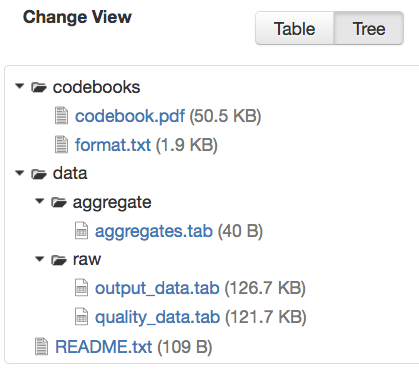
\includegraphics[scale=0.5]{cam.png}
            \label{Caminho}
        \end{figure}
  \noindent {\small Fonte: DATAVERSE PROJECT, 2019}
  
        \subsubsection{Tags do Arquivo}
        
\qquad As tags de arquivo são compostas por tags personalizadas de categoria, (documentação, dados, código) e de tabela (evento, genômica, geoespacial, rede, painel, pesquisa, série temporal). Use os menus suspensos de seleção e a entrada de tag de arquivo personalizada para aplicar essas tags aos arquivos selecionados. Há também um recurso Excluir Tags que, se marcado, permitirá que você exclua as tags de arquivo não utilizadas dentro desse conjunto de dados.
        
    \subsection{Substituir Arquivo}
    
\qquad Nos casos em que você deseja revisar um arquivo existente, em vez de adicionar um novo, é possível fazê-lo usando o recurso Substituir arquivo. Isso permitirá que você acompanhe o histórico desse arquivo nas versões do seu conjunto de dados, antes e depois de substituí-lo. Isso pode ser útil para atualizar seus dados ou corrigir erros nos dados. Como a substituição de um arquivo cria um link explícito entre a versão anterior do conjunto de dados e a versão atual, o recurso de substituição de arquivo não está disponível para rascunhos de conjuntos de dados não publicados. Observe também que a substituição de um arquivo não carrega automaticamente os metadados desse arquivo, mas, uma vez que o arquivo é substituído, seus metadados originais ainda podem ser encontrados fazendo referência à versão anterior do arquivo na guia "Versões" da página do arquivo.

Para substituir um arquivo, vá para a página do arquivo, clique no botão "Edit (Editar)" e, na lista suspensa, selecione "Replace (Substituir)". Isso o levará à página Substituir arquivo, onde você poderá ver os metadados da versão mais recente publicada do arquivo e fazer upload do seu arquivo de substituição. Depois de fazer o upload do arquivo de substituição, você poderá editar seu nome, descrição e tags. Quando terminar, clique no botão "Save Changes (Salvar alterações)".

Após a substituição bem-sucedida de um arquivo, será criada uma nova versão de rascunho do conjunto de dados. Um resumo de suas ações será gravado na guia "Versões", na página do conjunto de dados e na página do arquivo. A guia Versões permite acessar todas as versões anteriores do arquivo em todas as versões anteriores do seu conjunto de dados, incluindo a versão antiga do arquivo antes de substituí-lo.
    
    \subsection{Termos}
    
\qquad Os termos do conjunto de dados podem ser visualizados e editados na guia Termos da página do conjunto de dados ou no botão suspenso Editar de um conjunto de dados. Lá, você pode configurar como os usuários podem usar seus dados depois de baixá-los (renúncia CC0 ou Termos de Uso personalizados), como eles podem acessar seus dados se você tiver arquivos restritos (termos de acesso) e ativar um Livro de Visitas para o seu conjunto de dados, para que você possa rastrear quem está usando seus dados e para quais finalidades.
    
        \subsubsection{CC0 Domínio Público Dedicação}
        
\qquad Por padrão, todos os novos conjuntos de dados criados pela interface do usuário da web do Dataverse recebem uma Dedicação de Domínio Público Creative Commons CC0.

Se um proprietário de dados achar que CC0 não é adequado para seus dados, poderá inserir Termos de Uso personalizados.
    
        \subsubsection{Termos de Uso Customizados para Datasets}
        
\qquad Se você não conseguir usar a Dedicação ao Domínio Público CC0 em seus conjuntos de dados, poderá especificar seus próprios Termos de Uso personalizados. Para fazer isso, selecione “Não, não aplique CC0 -“ Dedicação ao domínio público ”, e uma caixa de texto Termos de uso será exibida, permitindo que você insira seus próprios termos de uso personalizados para o seu conjunto de dados. Para adicionar mais informações sobre os Termos de Uso, fornecemos campos como Permissões Especiais, Restrições, Requisitos de Citação, etc.
        
        \subsubsection{Arquivos Restritos + Termos de Acesso}
        
\qquad Se você restringir qualquer arquivo no seu conjunto de dados, será solicitado um pop-up para inserir os Termos de Acesso para os dados. Isso também pode ser editado na guia Termos ou selecionando Termos no botão suspenso "Edit (Editar)" no conjunto de dados. Você também pode permitir que os usuários solicitem acesso aos seus arquivos restritos, ativando "Solicitar acesso". Para adicionar mais informações sobre os Termos de acesso, fornecemos campos como Local de acesso a dados, Status de disponibilidade, Contato para acesso, etc.
        
        \subsubsection{Livro de Visitas}
        
\qquad Aqui se habilita o Livro de Visitas específico para o seu conjunto de dados, que é configurado no nível do Dataverse.

        \subsubsection{Nível de Dataset}
        
\qquad Os administradores ou curadores de um conjunto de dados podem atribuir funções e permissões aos usuários desse conjunto de dados. Se você é administrador ou curador de um conjunto de dados, pode acessar a página de permissões do conjunto de dados clicando no botão "Edit (Editar)", realçando "Permissões" na lista suspensa e clicando em " Dataset (Conjunto de dados)".\\

Ao acessar a página de permissões de um conjunto de dados, você verá duas seções:\\

\textbf{Usuários / grupos:} aqui você pode atribuir funções a usuários ou grupos específicos, determinando quais ações eles têm permissão para executar no seu conjunto de dados. Você também pode fazer referência a uma lista de todos os usuários que têm funções atribuídas a eles para o seu conjunto de dados e remover as funções, se desejar. Alguns dos usuários listados podem ter funções atribuídas no nível do dataverse, nesse caso, essas funções podem ser removidas apenas da página de permissões do dataverse.\\

\textbf{Funções:} Aqui você pode fazer referência a uma lista completa de funções que podem ser atribuídas aos usuários do seu conjunto de dados. Cada função lista as permissões que oferece.
        
        \subsubsection{Nível de Arquivo}
        
\qquad Se arquivos específicos no seu conjunto de dados tiverem acesso restrito, você poderá conceder acesso a usuários ou grupos específicos a esses arquivos, mantendo-os restritos ao público em geral. Se você é administrador ou curador de um conjunto de dados, pode acessar a página de permissões no nível do arquivo clicando no botão "Edit (Editar)", realçando "Permissões" na lista suspensa e clicando em "Arquivo".

Ao acessar a página de permissões no nível do arquivo de um conjunto de dados, você verá duas seções:\\

\textbf{Usuários / Grupos:} Aqui você pode ver quais usuários ou grupos tiveram acesso a quais arquivos. Você pode clicar no botão "Conceder acesso a usuários / grupos" para ver uma caixa onde você pode conceder acesso a arquivos específicos dentro do seu conjunto de dados para usuários ou grupos específicos. Se algum usuário tiver solicitado acesso a um arquivo no seu conjunto de dados, você poderá conceder ou rejeitar a solicitação de acesso aqui.\\

\textbf{Arquivos restritos:} Nesta seção, você pode ver as mesmas informações, mas discriminadas por cada arquivo individual no seu conjunto de dados. Para cada arquivo, você pode clicar no botão "Atribuir acesso" para ver uma caixa onde você pode conceder acesso a esse arquivo para usuários ou grupos específicos.
        
    \subsection{Proveniência dos Dados}
    
\qquad A proveniência de dados é um registro de onde seus dados vieram e como atingiram sua forma atual. Ele descreve a origem de um arquivo de dados, quaisquer transformações feitas nesse arquivo e quaisquer pessoas ou organizações associadas a esse arquivo. A proveniência de um arquivo de dados pode ajudar na reprodutibilidade e conformidade com os regulamentos legais. O Dataverse disponibiliza apenas informações de proveniência para aqueles que têm permissões de edição no seu conjunto de dados.

O Dataverse aceita informações de proveniência de duas formas: um Arquivo de proveniência ou uma Descrição de proveniência de texto livre. Você pode anexar essas informações de proveniência aos seus arquivos de dados no Dataverse como parte do processo de upload do arquivo, clicando em Editar -> Proveniência:
   
  \begin{figure}[H]
     \caption{Proveniência}
                \centering
         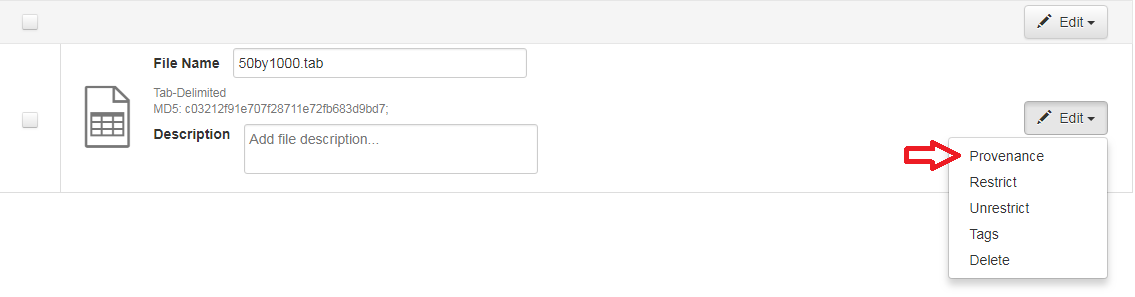
\includegraphics[scale=0.5]{prov.png}
            \label{Proveniência}
        \end{figure}
   \noindent {\small Fonte: DATAVERSE PROJECT, 2019}\\

Isso abrirá uma janela onde você pode adicionar seu arquivo de proveniência e / ou descrição da proveniência:
    
 \begin{figure}[H]
                 \caption{Arquivo de proveniência}
                \centering                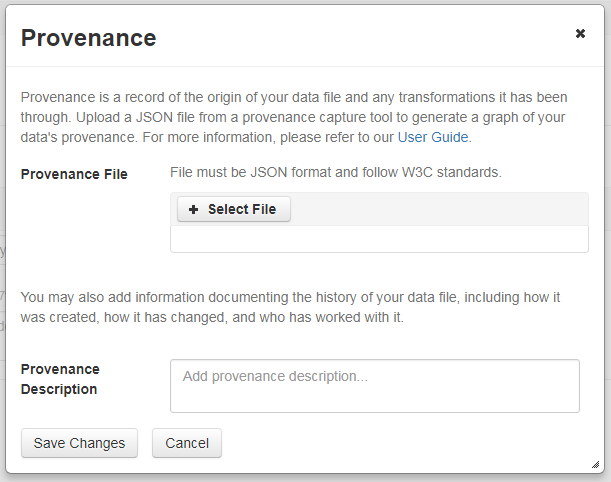
\includegraphics[scale=0.7]{prov1.png}
            \label{Proveniência1}
        \end{figure}
\noindent {\small Fonte: DATAVERSE PROJECT, 2019}\\

Depois de fazer o upload de um arquivo de proveniência, o Dataverse precisará de algumas informações adicionais para conectá-lo com precisão ao seu arquivo de dados. Quando o upload do arquivo de origem terminar, uma caixa de entrada chamada “Connect entity” aparecerá sob o arquivo. Os arquivos de proveniência contêm uma lista de "entidades", que incluem seu arquivo de dados e quaisquer objetos associados a ele (por exemplo, um gráfico, um corretor ortográfico, etc.). Você precisará informar ao Dataverse qual entidade no arquivo de proveniência representa seu arquivo de dados. Você pode digitar o nome da entidade na caixa ou clicar na seta ao lado da caixa e selecionar a entidade em uma lista de todas as entidades no arquivo de proveniência.

Depois de fazer o upload do seu arquivo de proveniência e conectar a entidade adequada, você pode clicar no botão "Visualizar" para visualizar o JSON bruto do arquivo de proveniência. Isso pode ajudar a confirmar que você enviou o arquivo certo. Verifique-o novamente, porque o arquivo de proveniência será permanente assim que for finalizado. Nesse ponto, você não poderá substituir, remover ou editar o arquivo de proveniência. Isso garante que o arquivo de proveniência mantenha um registro estável e imutável do histórico do arquivo de dados. 

Essa finalização do arquivo de proveniência ocorre em diferentes pontos, dependendo do status do seu arquivo de dados. Se este for um novo arquivo de dados que nunca foi publicado antes, o arquivo de proveniência associado será tornado permanente assim que você publicar o conjunto de dados. Se esse arquivo de dados foi publicado em uma versão anterior do seu conjunto de dados, o arquivo de proveniência associado será tornado permanente assim que você fizer o upload do arquivo de proveniência e clique em "Save Changes (Salvar alterações)" no pop-up de aviso.

Uma Descrição de proveniência permite adicionar mais informações de proveniência além ou no lugar de um arquivo de proveniência. Este é um campo de texto livre que permite que você insira qualquer informação que considere relevante para os interessados em aprender sobre a procedência de seus dados. Esse pode ser um bom lugar para descrever fatores de proveniência, como qual sistema operacional você usou ao trabalhar com o arquivo de dados, quais funções ou bibliotecas você usou, como os dados foram mesclados no arquivo, qual versão do arquivo você usou etc. A descrição não é tão útil ou confiável quanto um arquivo de proveniência, mas ainda pode fornecer valor. Ao contrário do arquivo de proveniência, a descrição da proveniência nunca é permanente: você sempre pode editá-lo, removê-lo ou substituí-lo a qualquer momento.

Você pode retornar para anexar a proveniência ao seu arquivo de dados posteriormente, clicando no botão "Add + Edit Metadata (Adicionar + Editar Metadados)" na página do arquivo e, em seguida, clicando no botão "Edit -> Provenance (Editar -> Origem)".
    
    \subsection{Thumbnails e Widgets}
    
        \subsubsection{Thumbnails}
        
\qquad As imagens em miniatura podem ser atribuídas a um conjunto de dados manual ou automaticamente. A miniatura de um conjunto de dados aparece no cartão de resultados da pesquisa para esse conjunto de dados e na própria página do conjunto de dados. Se um conjunto de dados contiver um ou mais arquivos de dados que o Dataverse reconheça como uma imagem, uma dessas imagens será selecionada automaticamente como miniatura do conjunto de dados.

Se você deseja selecionar manualmente a miniatura do seu conjunto de dados, clique no botão "Edit (Editar)" no seu conjunto de dados e selecione "Miniaturas + Widgets" no menu suspenso.\\

Nesta página, na guia Miniatura, você verá três ações possíveis.\\

\textbf{Selecionar arquivo disponível:} clique no botão "Selecionar miniatura" para \\escolher uma imagem do seu conjunto de dados para usá-la como miniatura do conjunto de dados.\\

\textbf{Carregar novo arquivo:} carregue um arquivo de imagem do seu computador para usá-lo como miniatura do conjunto de dados. Embora, por padrão, sua imagem em miniatura seja desenhada a partir de um arquivo no seu conjunto de dados, isso permitirá que você envie um arquivo de imagem separado para usar como miniatura do conjunto de dados. Este arquivo de imagem enviado será usado apenas como miniatura do conjunto de dados, ele não será armazenado como um arquivo de dados no seu conjunto de dados.\\

\textbf{Remover miniatura:} se você clicar no botão "Remove (Remover)" abaixo da imagem em miniatura, removerá a miniatura atual do conjunto de dados. O conjunto de dados será revertido para exibir um ícone padrão básico como miniatura do conjunto de dados.

Quando terminar nesta página, clique em "Save Changes (Salvar alterações)" para salvar o que você fez. Se preferir, também é possível definir um arquivo de imagem em seu conjunto de dados como miniatura, selecionando o arquivo, indo em Edit Files -> Metadata e usando o botão "Set Thumbnail".
        
        \subsubsection{Widgets}
        
\qquad O recurso Widgets fornece código para seu site pessoal, para que seu conjunto de dados possa ser exibido. Existem dois tipos de Widgets para um conjunto de dados: o Widget do Conjunto de Dados e o Widget de Citação do Conjunto de Dados. Os widgets podem ser encontrados indo para a página do conjunto de dados, clicando no botão "Edit (Editar)" (aquele com o ícone de lápis) e selecionando "Miniaturas + Widgets" no menu suspenso.

Na guia Widgets, você pode copiar e colar os trechos de código do widget que você deseja adicionar ao seu site. Se você precisar ajustar a altura do widget em seu site, poderá fazê-lo editando o parâmetro heightPx = 500 no snippet de código.

        \subsubsection{Widget dataset}
        
\qquad O Widget do conjunto de dados permite que a citação, metadados, arquivos e termos do seu conjunto de dados sejam exibidos no seu site. Quando alguém baixa um arquivo de dados no widget, ele é baixado diretamente dos conjuntos de dados no seu site. Se um arquivo for restrito, eles serão direcionados ao seu dataverse para efetuar login, em vez de fazer login através do widget em seu site.

Para editar seu conjunto de dados, você precisará retornar ao repositório do Dataverse onde o conjunto de dados está armazenado. Você pode fazer isso facilmente clicando no link "Data Stored in (Name) Dataverse (Dados armazenados no (nome) dataverse)" localizado na parte inferior do widget.
        
        \subsubsection{Widget Citação de dataset}
        
\qquad O Widget de Citação do Conjunto de Dados fornecerá uma citação para o seu conjunto de dados no site pessoal ou do projeto. Os usuários podem baixar a citação em vários formatos usando o botão Citar Dados. O URL persistente na citação direcionará os usuários para o conjunto de dados no seu dataverse.
        
    \subsection{Publique Datasets}
    
\qquad Ao publicar um conjunto de dados (disponível para um administrador, curador ou qualquer função personalizada que tenha esse nível de permissão atribuído), você o disponibiliza ao público geral para que outros usuários possam procurá-lo. Quando seu conjunto de dados estiver pronto para ser publicado, vá para a página do seu conjunto de dados e clique no botão "Publish (Publicar)" no lado direito da página. Um pop-up aparecerá para confirmar que você está realmente pronto para publicar, pois uma vez que um conjunto de dados é tornado público, ele não pode mais ser publicado.

Sempre que você edita seu conjunto de dados, você pode publicar uma nova versão do conjunto de dados. O botão Publicar conjunto de dados reaparecerá sempre que você editar os metadados do conjunto de dados ou adicionar um arquivo.

Antes de publicar seu conjunto de dados, a Citação de dados indicará que este é um rascunho, mas o texto "DRAFT VERSION" será removido assim que você publicar.
    
    \subsection{Submeter à Revisão}
    
\qquad Se você tiver uma função de Colaborador (pode editar metadados, fazer upload e editar arquivos, editar Termos, Livro de Visitas e Enviar conjuntos de dados para revisão) em um Dataverse, poderá enviar seu conjunto de dados para revisão quando terminar de enviar e preencher todos os dados. dos campos de metadados relevantes. Para enviar para revisão, vá para o seu conjunto de dados e clique no botão "Submit for Review (Enviar para revisão)", localizado ao lado do botão "Edit (Editar)" no canto superior direito. Depois de enviado para revisão: o administrador ou o curador deste Dataverse será notificado para revisar esse conjunto de dados antes de decidir "Publicar" o conjunto de dados ou "Retornar ao autor". Se o conjunto de dados for publicado, o colaborador receberá uma notificação dizendo que o mesmo agora se encontra publicado. Se o conjunto de dados for retornado ao autor, o colaborador desse conjunto de dados será notificado que precisa fazer modificações antes de poder ser enviado para revisão novamente.
    
    \subsection{URL Privada para Revisão de Datasets Não publicados}
    
\qquad A criação de uma URL privada para o seu conjunto de dados permite que você compartilhe seu conjunto de dados (para visualização e download de arquivos) antes de ser publicado para um amplo grupo de indivíduos que podem não ter uma conta de usuário no Dataverse. Qualquer pessoa para quem você enviar o URL privado não precisará fazer login no Dataverse para visualizar o conjunto de dados:\\

1. Vá para o seu conjunto de dados não publicado\\

2. Selecione o botão " Edit (Editar)"\\

3. Selecione "Private URL (URL privado)" no menu suspenso\\

4. No pop-up, selecione "Create Private URL (Criar URL privado)"\\

5. Copie o URL privado que foi criado para este conjunto de dados e agora pode ser compartilhado com qualquer pessoa que você deseja ter acesso para exibir ou baixar arquivos no seu conjunto de dados não publicado.\\

Para desativar um URL privado e revogar o acesso, siga as mesmas etapas acima até a etapa 3, quando você retornar ao pop-up, clique no botão "Disable Private URL (Desativar URL privada)".
    
    \subsection{Versões dos Datasets}
    
\qquad O controle de versão é importante para o gerenciamento de dados de pesquisa de longo prazo, onde os metadados e / ou arquivos são atualizados ao longo do tempo. É usado para rastrear quaisquer metadados ou alterações de arquivo (por exemplo, fazendo upload de um novo arquivo, alterando metadados de arquivo, adicionando ou editando metadados) após a publicação do conjunto de dados.

\begin{figure}[H]
    \caption{Versões}
    \centering
      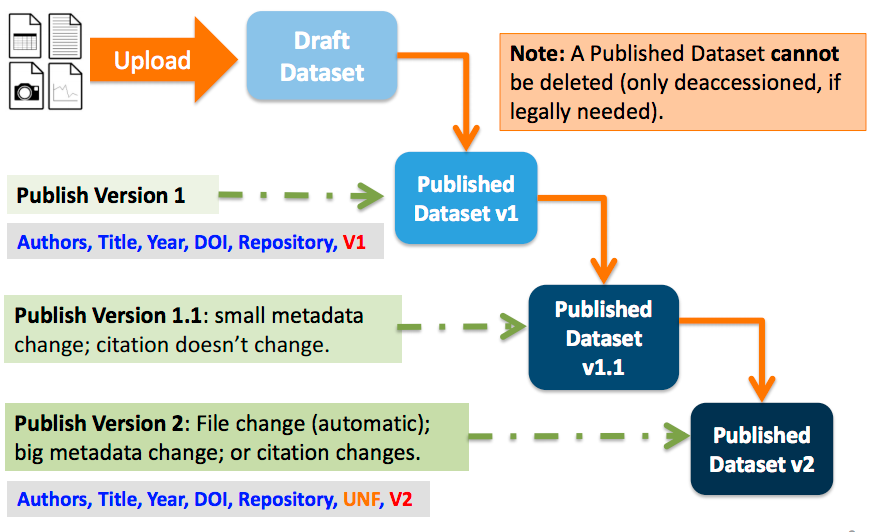
\includegraphics[scale=0.4]{ver.png}
    \label{Versão}
 \end{figure}
\noindent Fonte: DATAVERSE PROJECT\\
    
Depois de editar seu conjunto de dados publicado, uma nova versão de rascunho desse conjunto de dados será criada. Para publicar esta nova versão do seu conjunto de dados, selecione o botão "Publish Dataset (Publicar conjunto de dados)" no canto superior direito da página. Se você estivesse na versão 1 do seu conjunto de dados, dependendo dos tipos de alterações feitas, seria solicitado publicar seu rascunho como versão 1.1 ou versão 2.0.

Se você adicionar um arquivo, seu conjunto de dados será automaticamente atualizado para uma versão principal (por exemplo, se você estivesse na versão 1.0, irá para a versão 2.0).

Na guia Versões de uma página de conjunto de dados, há uma tabela de versões que exibe o histórico de versões do conjunto de dados. Você pode usar os links do número da versão nesta tabela para navegar entre as diferentes versões do conjunto de dados, incluindo a versão de rascunho não publicada, se tiver permissão para acessá-lo.

Há também uma guia Versões na página do arquivo. A tabela de versões para um arquivo exibe as mesmas informações que o conjunto de dados, mas os resumos são filtrados para mostrar apenas as ações relacionadas a esse arquivo. Se uma nova versão do conjunto de dados fosse criada sem nenhuma alteração em um arquivo individual, o resumo da versão do arquivo para essa versão do conjunto de dados seria "Nenhuma alteração associada a esta versão".
    
         \subsubsection{Detalhes das Versões}
         
\qquad Para visualizar exatamente o que mudou, iniciando da versão publicada originalmente para as versões publicadas subsequentes: clique na guia Versões na página do conjunto de dados para ver todas as versões e alterações feitas para esse conjunto de dados específico.

Depois de ter mais de uma versão (pode ser simplesmente a versão 1 e um rascunho), você pode clicar no link "View Details (Visualizar detalhes)" ao lado de cada resumo para saber mais sobre os campos e arquivos de metadados que foram adicionados ou editados. Você também pode clicar nas caixas de seleção para selecionar duas versões do conjunto de dados e clicar no botão "View Differences (Exibir diferenças)" para abrir o pop-up Detalhes das diferenças de versão e comparar as diferenças entre elas.
         
    \subsection{Desativar acessos de Dataset}
    
\qquad Não é recomendável desativar um conjunto de dados ou uma versão de um conjunto de dados. Se você absolutamente precisar desacessar, poderá desativar uma versão de um conjunto de dados ou de um conjunto de dados inteiro.
Para desacessar, vá para o conjunto de dados publicado (ou adicione um novo e publique-o), clique no botão "Edit (Editar)" e, no menu suspenso, selecione "Deaccession Dataset (Desacessar dataset)". Se você tiver várias versões de um conjunto de dados, poderá selecionar aqui quais versões deseja desativar ou optar por desativar todo o conjunto de dados.

Você também deve incluir um motivo pelo qual esse conjunto de dados foi desativado. Selecione o motivo mais apropriado na lista suspensa de opções. Se você selecionar “Outro”, também deverá fornecer informações adicionais.

Adicione mais informações sobre o motivo por que foi desativado na caixa de texto livre. Se o conjunto de dados foi movido para um repositório ou site diferente, recomendamos que você inclua uma URL (de preferência persistente) para que os usuários possam continuar acessando esse conjunto de dados no futuro.

Se você desativar a versão publicada mais recentemente do conjunto de dados, mas nem todas as versões do conjunto de dados, poderá revisitar uma versão anterior e criar um novo rascunho não desativado para o conjunto de dados. Por exemplo, imagine que você tenha a versão 1 e a versão 2 de um conjunto de dados, ambas publicadas, e a versão 2 desacessada. Você poderá editar a versão 1 do conjunto de dados e uma nova versão de rascunho será criada.

Uma página de lápide com os metadados básicos de citação sempre estará acessível ao público se eles usarem o URL persistente (Handle ou DOI) fornecido na citação para esse conjunto de dados. Os usuários não poderão ver nenhum dos arquivos ou metadados adicionais que estavam disponíveis anteriormente antes da desativação.
        
\newpage

\section{Manual do administrador}
\vspace{10.5cm}

\newpage

    \subsection{Painel de controle}
    
\qquad O Dataverse oferece um painel de ferramentas administrativas apenas para  superusuários. Se você é um superusuário logado, pode acessá-lo clicando no seu nome de usuário na barra de navegação e, em seguida, clicando em "Dashboard" no menu suspenso, fig. \ref{img01.png}.


\begin{figure}[!htp]
    \centering
      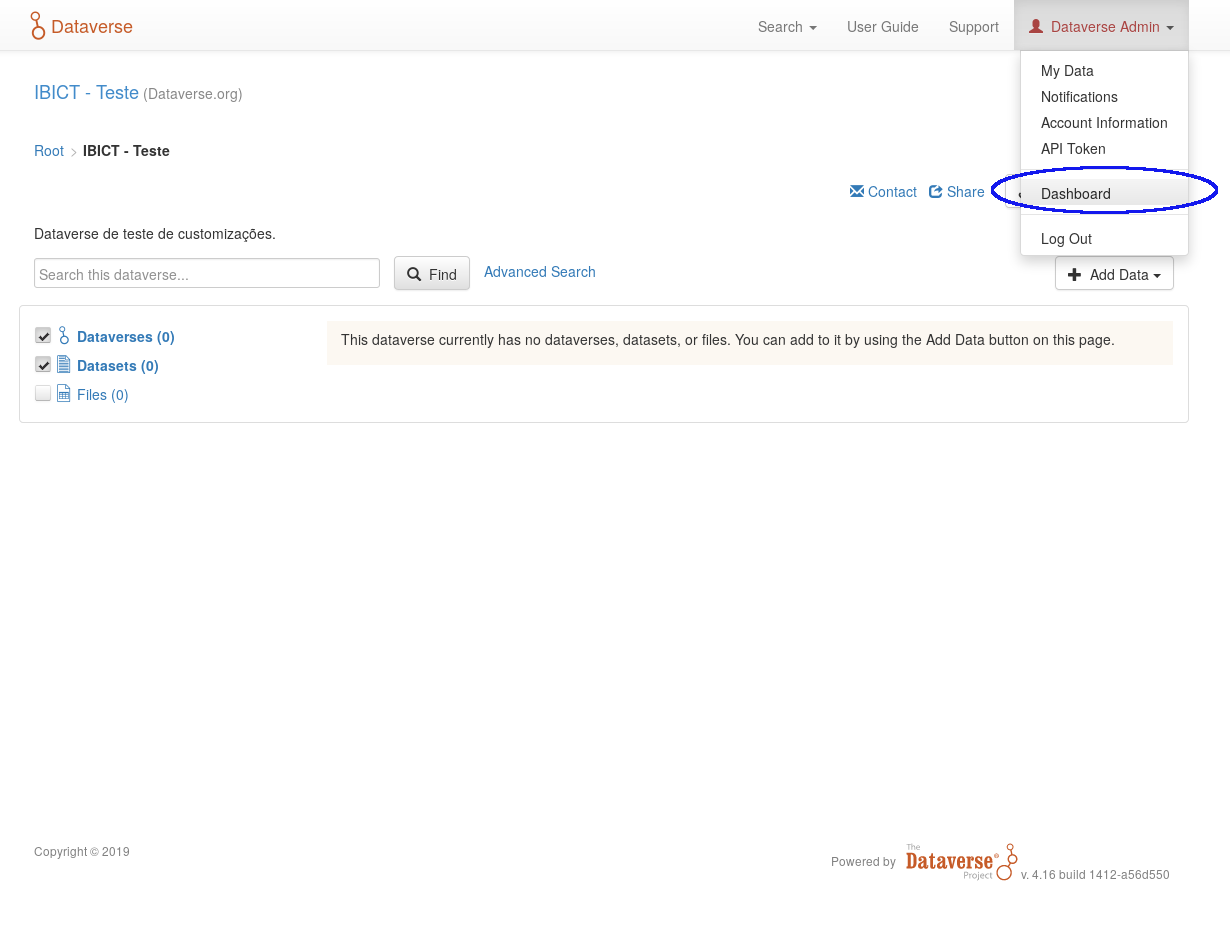
\includegraphics[scale=0.2]{imagens/01.png}
        \caption{Dashboard}
    \label{img01.png}
 \end{figure}

Você pode verificar se é um superusuário, verificando a cor do seu nome de usuário na barra de navegação. Se estiver vermelho, você tem as permissões corretas para usar o Painel. Os superusuários podem fornecer a outros usuários o status de superusuário via Administração do Usuário.

\subsubsection{Harvest}

\qquad\textbf{Coletando Clientes}\\

Essa ferramenta de painel permite configurar de quais outros repositórios sua instalação do Dataverse coleta registros de metadados. Você pode visualizar uma lista de clientes de coleta e adicioná-los, editar ou removê-los.\\



\textbf{Coletando Servidores}\\

Essa ferramenta de painel permite definir conjuntos de conjuntos de dados locais para disponibilizar aos clientes de coleta remota. Você pode ver uma lista de conjuntos e adicioná-los, editar ou removê-los.

Depois de clicar na opção Dashboard, fig.\ref{img01.png}, o site abrirá uma janela com as opções, clique no \textit{Manager Server}, do item \textit{Harvest Server}, figura \ref{img02.png}. Na janela \textit{Harvest Server}, figura \ref{img04.png}, estão as informações básicas sobre o colate. 

Na parte logo acima da descrição tem o item \textit{OAI Server}. Este item estará desabilitado, agora, modifique sua opção para \textit{Enable}.
 
 \begin{figure}[ht]
\begin{subfigure}{.5\textwidth}
  \centering
  % include first image
  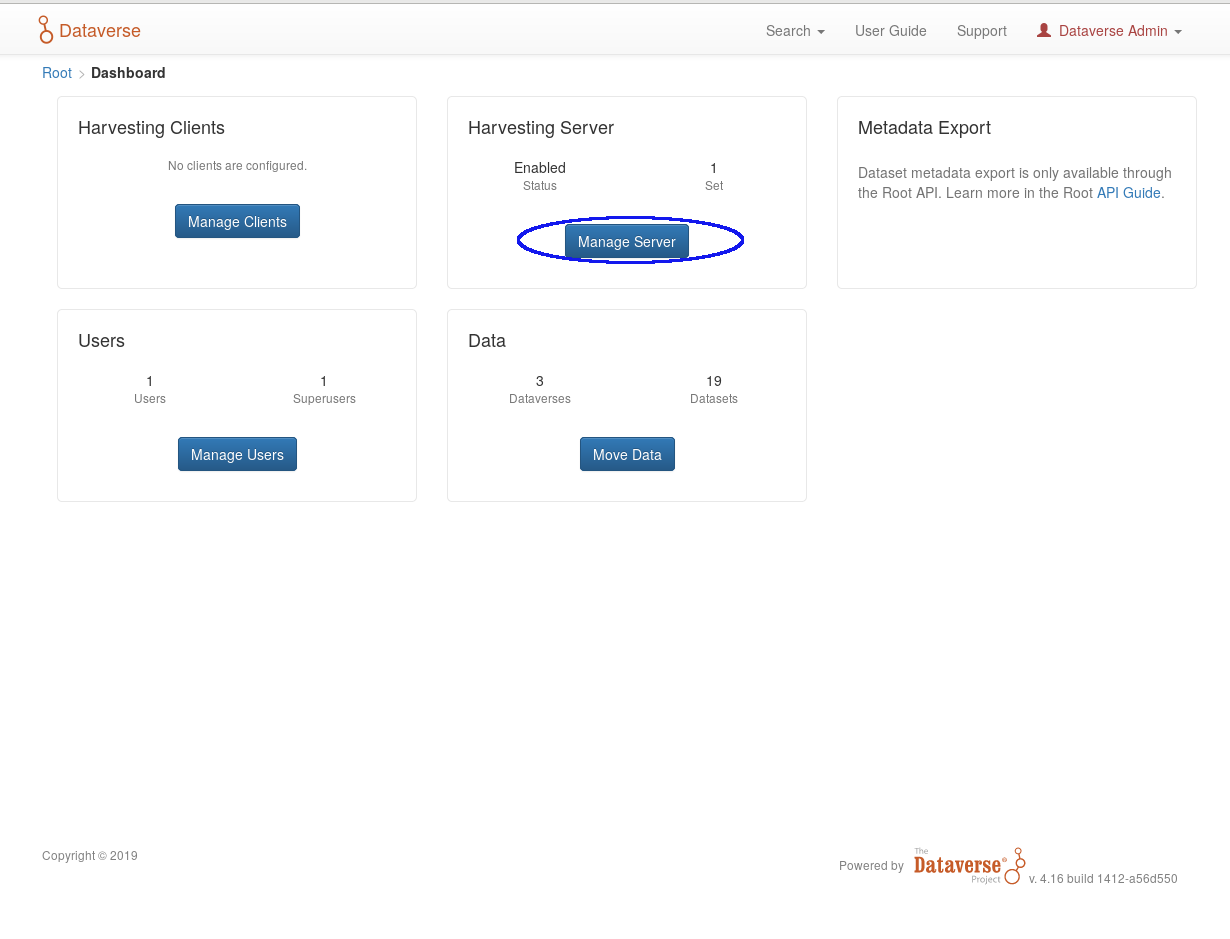
\includegraphics[width=.9\linewidth]{imagens/02.png}  
  \caption{Janela Dashboard}
  \label{img02.png}
\end{subfigure}
\begin{subfigure}{.5\textwidth}
  \centering
  % include second image
  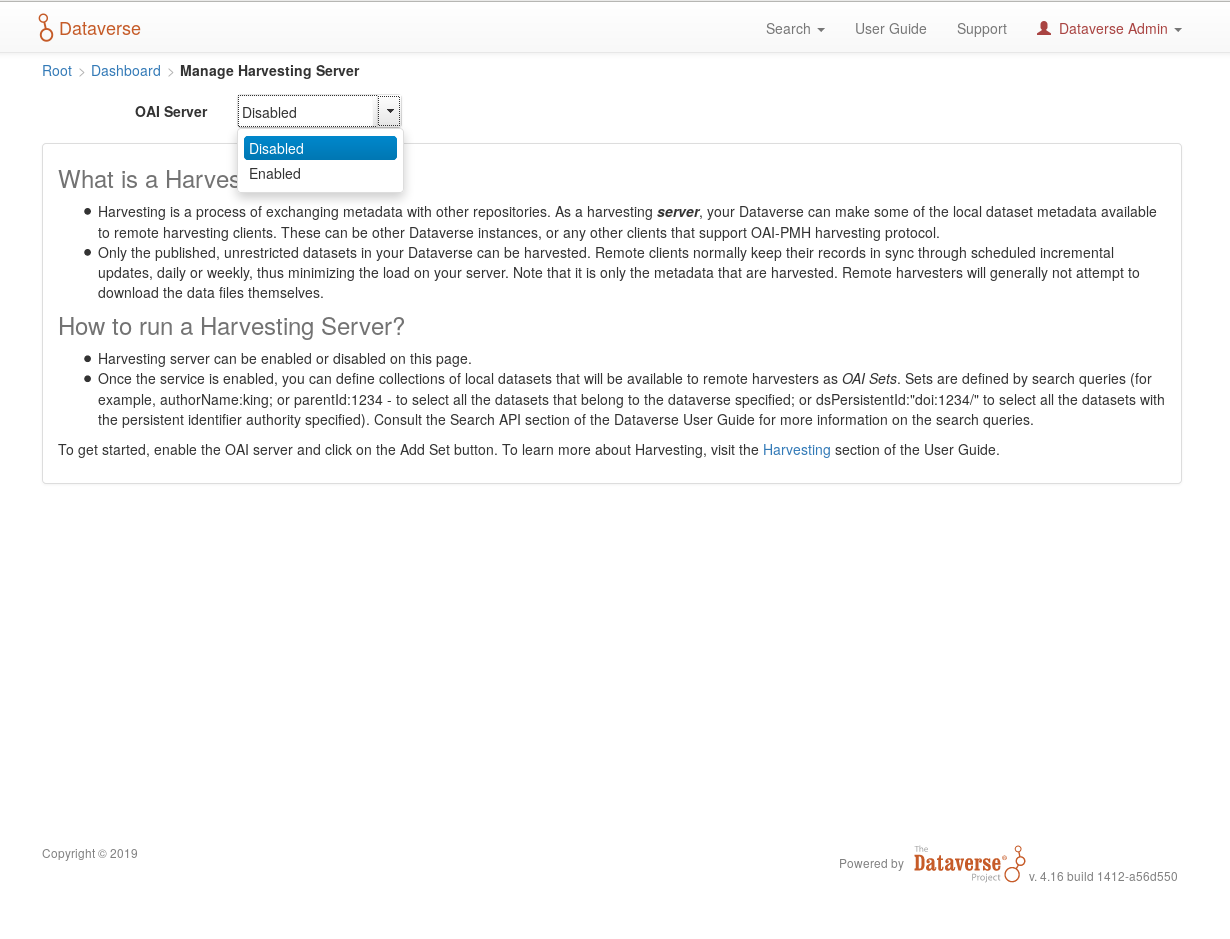
\includegraphics[width=.9\linewidth]{imagens/04.png}  
  \caption{Janela para habilitar o servidor OAI}
  \label{img03.png}
\end{subfigure}
\caption{Harvest server}
\label{img0203}
\end{figure}

Para verificar se foi modificado, acesse o endereço \textit{http://\color[red]{URL DO DATAVERSE}/oai}. Caso a página seja parecida com a figura \ref{img06.png}, o OAI server está habilitado.

\begin{figure}[!htp]
    \centering
      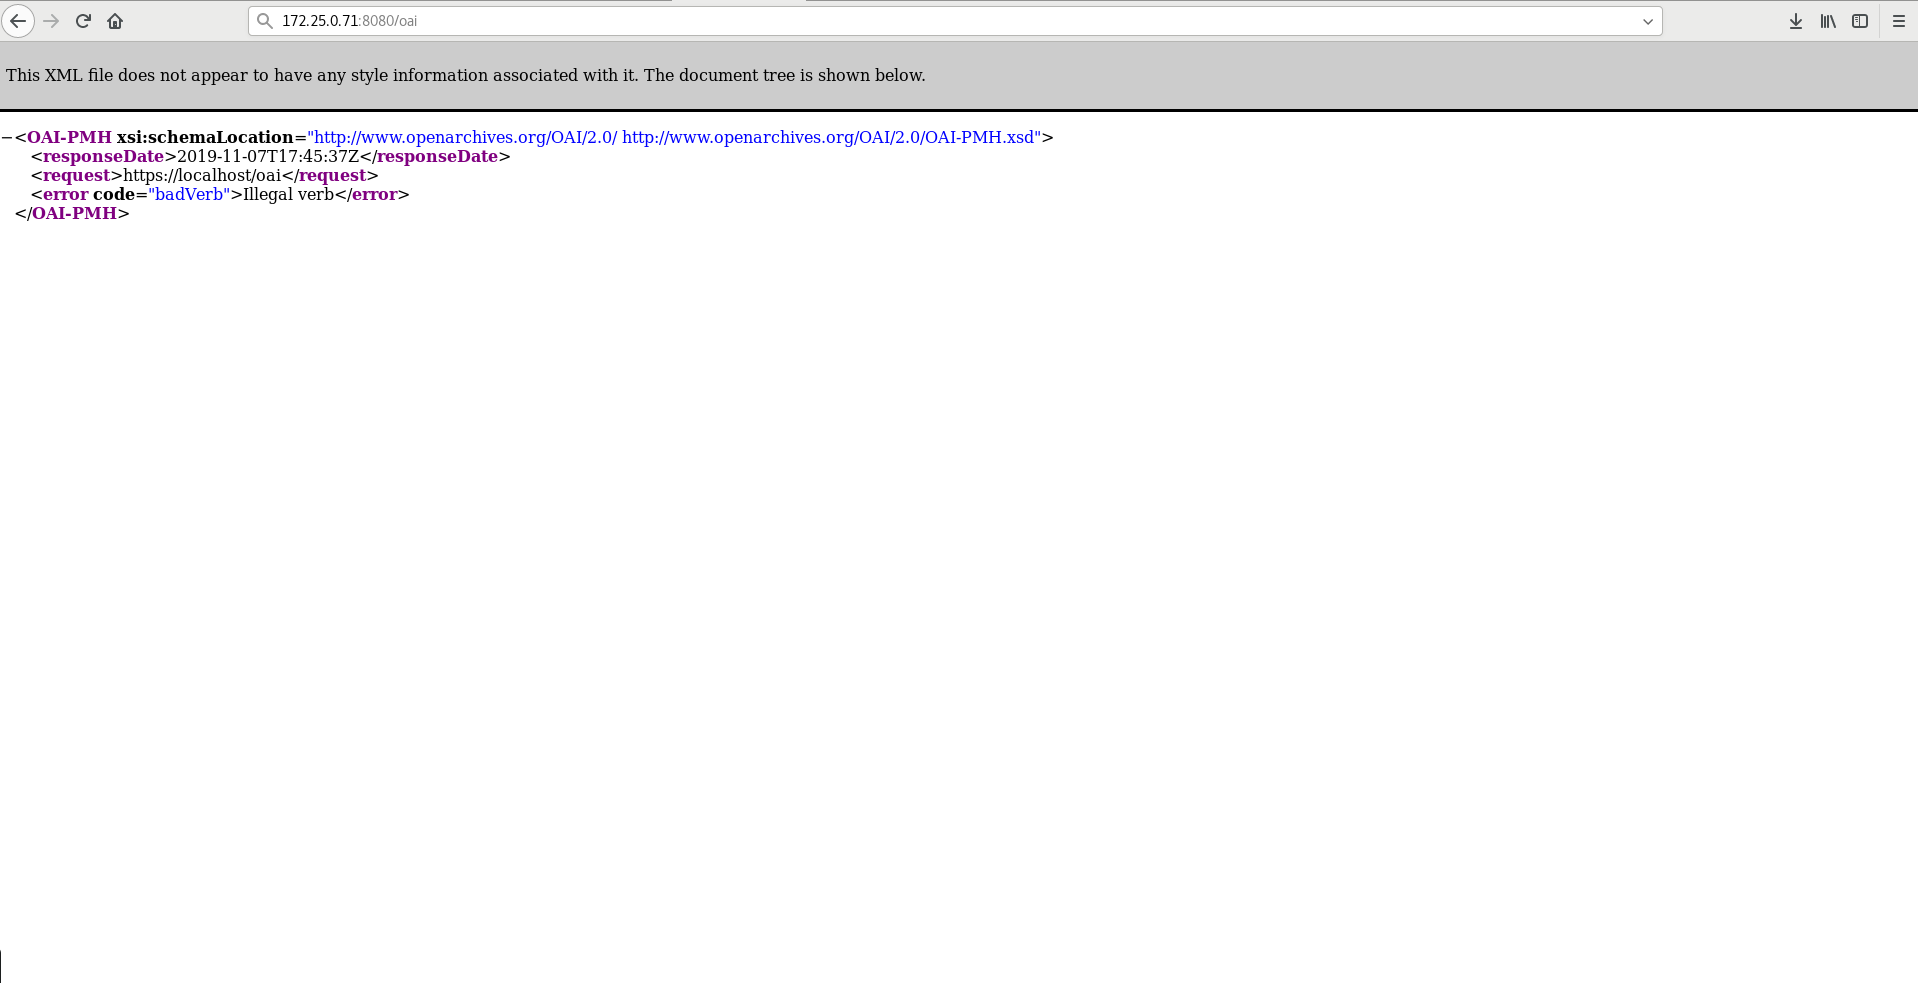
\includegraphics[scale=0.2]{imagens/06.png}
        \caption{Dashboard}
    \label{img06.png}
 \end{figure}

 \begin{figure}[ht]
\begin{subfigure}{.5\textwidth}
  \centering
  % include first image
  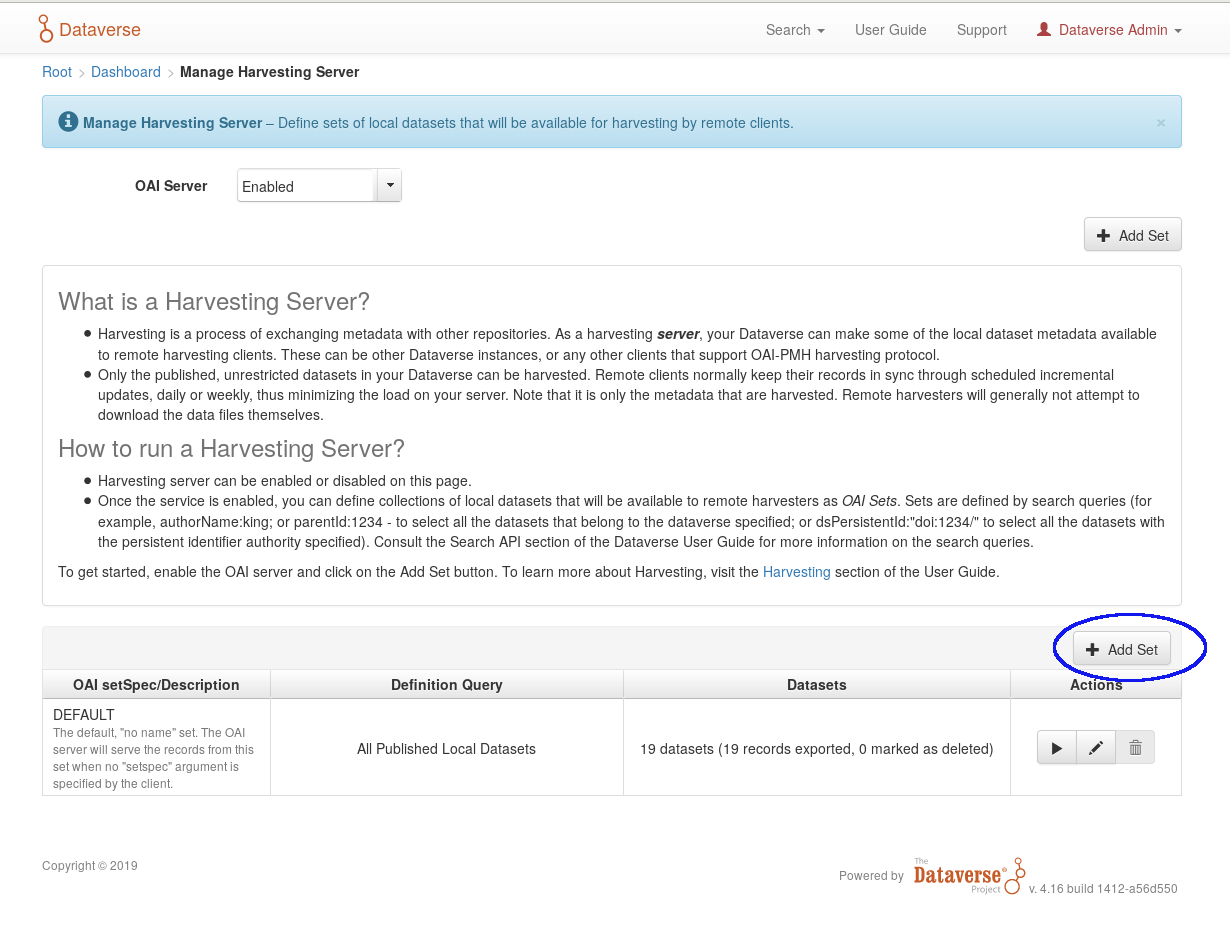
\includegraphics[width=.9\linewidth]{imagens/03.png}  
  \caption{Adicionar uma coleta}
  \label{img04.png}
\end{subfigure}
\begin{subfigure}{.5\textwidth}
  \centering
  % include second image
  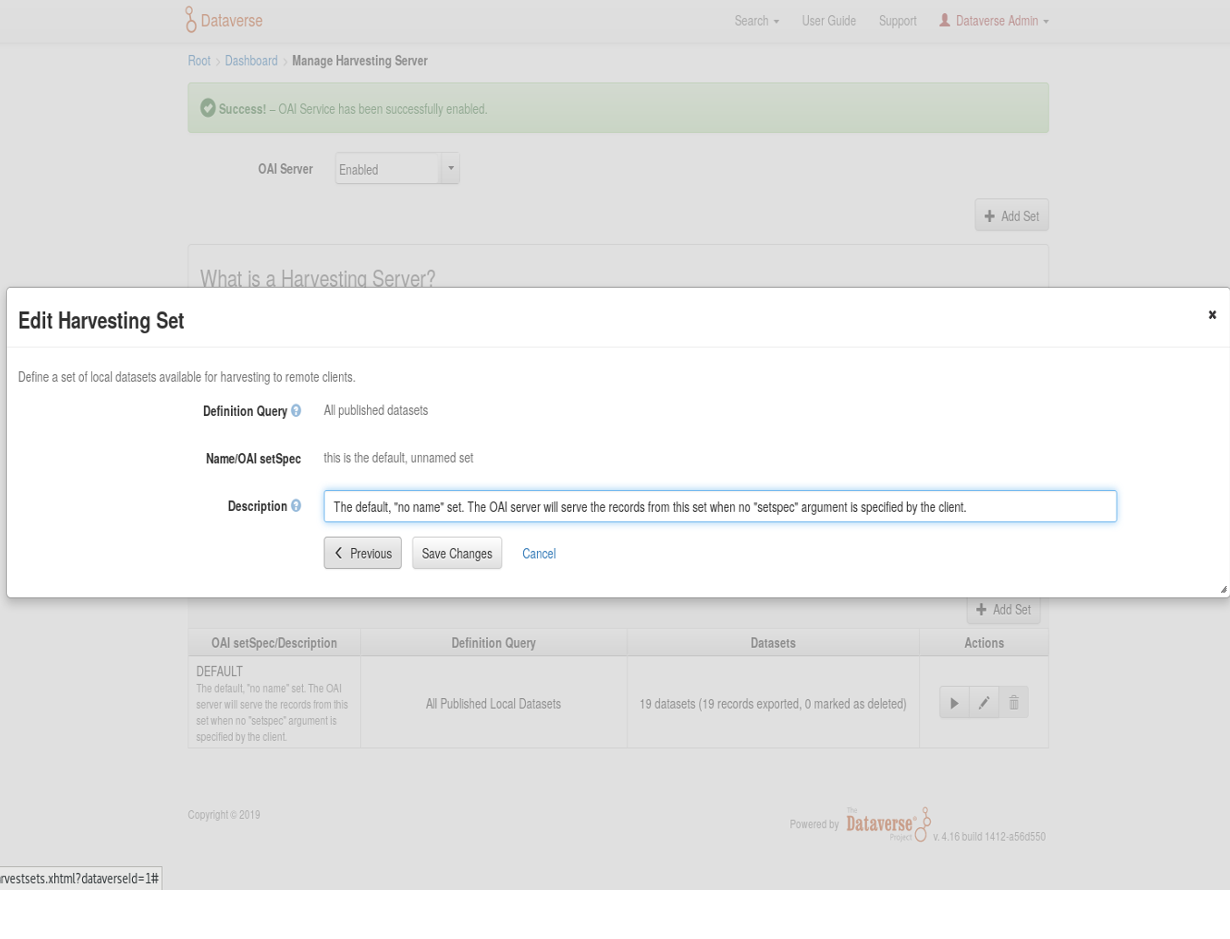
\includegraphics[width=.9\linewidth]{imagens/05.png}  
  \caption{Configurar coleta}
  \label{img05.png}
\end{subfigure}
\caption{Criar um critério de coleta}
\label{img0405}
\end{figure}
 
\newpage
\subsubsection{Usuários}

\qquad Essa ferramenta de painel permite pesquisar uma lista de todos os usuários da sua instalação do Dataverse. Você pode remover funções das contas de usuário e atribuir ou remover o status de superusuário.

\subsection{Gerenciando clientes de coleta}

\subsubsection{Seu Dataverse como um Harvester de Metadados}

\qquad A coleta é um processo de troca de metadados com outros repositórios. Como cliente de coleta, seu Dataverse pode coletar registros de metadados de fontes remotas. Podem ser outras instâncias do Dataverse ou outros arquivos que suportam OAI-PMH, o protocolo de coleta padrão. Os registros de metadados coletados serão indexados e tornados pesquisáveis por seus usuários. Clicar em um conjunto de dados coletado nos resultados da pesquisa leva o usuário ao repositório original. Conjuntos de dados coletados não podem ser editados na instalação do Dataverse.
 
Os registros coletados podem ser mantidos em sincronia com o repositório original por meio de atualizações incrementais agendadas, diariamente ou semanalmente. Como alternativa, as coletas podem ser executadas sob demanda pelo administrador.
 
\subsubsection{Gerenciando clientes de coleta}

\qquad Para começar a coletar metadados de um repositório OAI remoto, primeiro crie e configure um Harvesting Client.
 
Os clientes são gerenciados na página "coleta de clientes", acessível através do Painel. Clique no botão Adicionar cliente para começar.
 
O processo de criação de um novo cliente ou edição de um cliente existente é amplamente autoexplicativo. Ele é dividido em etapas lógicas, de forma que permita ao usuário voltar e corrigir as entradas feitas anteriormente. O processo é interativo e o texto de orientação é fornecido. Por exemplo, é necessário que o usuário insira a URL do servidor OAI remoto. Quando ele clica em Avançar, o aplicativo tenta estabelecer uma conexão com o servidor para verificar se está funcionando e para obter informações sobre os conjuntos de registros de metadados e os formatos de metadados que ele suporta. As opções oferecidas ao usuário na próxima página serão baseadas nessas informações extras. Se o aplicativo falhar ao estabelecer uma conexão com o arquivo remoto no endereço especificado, ou se uma resposta inválida for recebida, o usuário terá a oportunidade de verificar e corrigir o URL digitado.
 
\subsection{Gerenciando conjuntos e servidor de coleta}

\subsubsection{Seu Dataverse como servidor OAI}

\qquad Como servidor de coleta, seu Dataverse pode disponibilizar alguns dos metadados do conjunto de dados local para clientes de coleta remota. Podem ser outras instâncias do Dataverse ou quaisquer outros clientes que suportam o protocolo de coleta OAI-PMH.

\subsubsection{Como funciona?}

\qquad Somente os conjuntos de dados publicados e irrestritos no seu Dataverse podem ser colhidos. Os clientes remotos normalmente mantêm seus registros sincronizados por meio de atualizações incrementais agendadas, diariamente ou semanalmente, minimizando a carga no servidor. Observe que são apenas os metadados que são coletados. Os harvesters remotos geralmente não tentam baixar os arquivos de dados associados aos conjuntos de dados coletados.
O servidor de coleta pode ser ativado ou desativado na página "Servidor de coleta", acessível através do Painel. Por padrão, o servidor de coleta está desativado em um Dataverse novo e "pronto para uso".

\subsubsection{Conjuntos OAI}

\qquad Depois que o serviço é ativado, você define coleções de conjuntos de dados locais que estarão disponíveis para Harvester remotos como Conjuntos OAI. Os conjuntos são definidos por search queries. Qualquer consulta que encontre qualquer número de conjuntos de dados locais publicados (não coletados) pode ser usada para criar um conjunto OAI. Os conjuntos podem se sobrepor a locais de dados locais e podem incluir o número mínimo ou máximo de conjuntos de dados locais que você desejar.

Depois de inserir a search queries e clicar em Avançar, o número de resultados encontrados será mostrado na próxima tela. Dessa forma, se você perceber um número diferente do esperado, poderá voltar e tentar redefinir a consulta.\\

Alguns exemplos úteis de consultas de pesquisa para definir conjuntos OAI:

\begin{itemize}

 \item Uma boa maneira de criar um conjunto que inclua todos os seus conjuntos de dados locais publicados é fazê-lo pela autoridade Identificador Único registrada no seu Dataverse, por exemplo:
 
\begin{minted}{bash}

dsPersistentId: "doi: 1234 /"

\end{minted}

Observe que aspas duplas devem ser usadas, pois o valor do campo de pesquisa contém o símbolo de dois pontos.

Observe também que os termos de pesquisa que limitam os resultados aos conjuntos de dados publicados e locais são adicionados automaticamente à consulta. Portanto, você não precisa se preocupar com isso.

 \item Uma consulta para criar um conjunto para incluir os conjuntos de dados de uma coleta local específica:
 
\begin{minted}{bash}

parentId: NNN

\end{minted}

Em que NNN é o ID do banco de dados do objeto DataVerse (consulte a tabela Dataverse do banco de dados SQL usado pelo aplicativo para verificar o ID do banco de dados).

 \item Uma consulta para encontrar todo o conjunto de dados de um determinado autor:
 
\begin{minted}{bash}
 
authorName: YYY

\end{minted}

Onde AAA é o nome.

 \item Consultas complexas podem ser criadas com vários operadores lógicos AND e OR. Por exemplo,
 
 \begin{minted}{bash}
 
(authorName: YYY OR authorName: ZZZ) E dsPublicationDate: NNNN

\end{minted}

 \item Alguns exemplos adicionais de consulta:
Para conjuntos de dados específicos usando um persistentID:

\begin{minted}{bash}

(dsPersistentId: 10.5000 / 
ZZYYXX / OU dsPersistentId: 10.5000 / XXYYZZ)

\end{minted}

Para todos os conjuntos de dados em uma autoridade de ID específica:

 \begin{minted}{bash}

dsPersistentId: 10.5000 / XXYYZZ

\end{minted}

Para todos os dataverses com disciplinas de Astronomia e Astrofísica ou Ciências da Terra e do Ambiente:

\begin{minted}{bash}

(dvSubject: "Astronomia e astrofísica" OU
dvSubject: "Terra e ciências ambientais")

\end{minted}

Para todos os conjuntos de dados que contêm a palavra-chave "censura":

\begin{minted}{bash}

keywordValue: censura

\end{minted}

\end{itemize}

\subsubsection{Atualizações do conjunto OAI}

\qquad Sempre que um novo conjunto de coleta é criado ou são feitas alterações em um conjunto existente, o conteúdo do conjunto é atualizado automaticamente - o aplicativo Dataverse encontrará os conjuntos de dados definidos pela consulta e tentará executar a exportação de metadados nos que ainda não foram exportados. Somente os conjuntos de dados para os quais a exportação foi concluída com êxito e os resultados armazenados em cache no sistema de arquivos são incluídos nos conjuntos OAI anunciados aos clientes da coleta.

Observe, no entanto, que as alterações feitas nos metadados reais do conjunto de dados não acionam automaticamente nenhum conjunto OAI correspondente para ser atualizado imediatamente. Por exemplo: digamos que você criou um conjunto OAI definido pela consulta de pesquisa

\begin{minted}{bash}

authorName: king 

\end{minted}

Que resultou em 43 registros de conjunto de dados. Se um novo conjunto de dados do mesmo autor for adicionado e publicado, isso não adicionará imediatamente o registro extra ao conjunto. Simplesmente seria muito custoso atualizar todos os conjuntos sempre que forem feitas alterações nos metadados.

No entanto, o conjunto OAI será atualizado automaticamente por um trabalho agendado de exportação de metadados que é executado todas as noites (às 2h da manhã, por padrão). Esse cronômetro de exportação é criado e ativado automaticamente sempre que o aplicativo é implantado ou reiniciado.

Ainda é possível, no entanto, fazer alterações como essa serem imediatamente refletidas no servidor OAI, acessando a página do Harvesting Server e clicando no ícone "Executar exportação" ao lado do conjunto OAI desejado.

\subsection{Customização de metadados}

\qquad  O Dataverse possui um sistema flexível de metadados orientado a dados, alimentado por "blocos de metadados".

\subsubsection{Introdução}

\qquad Antes de iniciar a personalização de metadados no Dataverse, verifique a possibilidade de customização disponível na interface da web do Dataverse. É possível ocultar os campos e torná-los necessários, clicando em "Editar" no nível do dataverse, clicando em "Informações gerais" e fazendo ajustes em "Campos de metadados".\\

As possibilidades de personalização incluem:

\begin{itemize}

\item Editar e adicionar campos de metadados;

\item Edição e adição de texto instrucional (dicas de ferramentas de rótulos de campo e marcas d'água de caixa de texto);

\item Editar e adicionar vocabulários controlados;

\item Alterar os campos que os depositantes devem usar para salvar os conjuntos de dados;

\item Alterar como os valores salvos dos metadados são exibidos na interface do usuário.

\end{itemize}

De um modo geral, é mais seguro criar seu próprio bloco de metadados personalizado em vez de editar os blocos de metadados fornecidos com o Dataverse. Observe que os blocos de metadados enviados com o Dataverse são baseados em padrões (por exemplo, DDI para Ciências Sociais). O dataverse é enviado com um bloco de metadados de citação, que inclui campos obrigatórios necessários para atribuir IDs persistentes a conjuntos de dados e blocos de metadados específicos do domínio. As definições desses blocos são carregadas em uma instalação do Dataverse em valor separado por tabulação (TSV). Embora seja tecnicamente possível definir mais de um bloco de metadados em um arquivo TSV, é uma boa prática organizacional definir apenas um em cada arquivo.

\subsubsection{Sobre o bloco de metadados TSV}

 \qquad Os propósitos de cada seção e propriedade do bloco de metadados TSV são:\\

1. metadataBlock

\begin{itemize}
   
 \item Objetivo: Representa o bloco de metadados que está sendo definido.
 
 \item Cardinalidade:\\\\
0 ou mais por Dataverse\\\\
1 por definição de bloco de metadados

\end{itemize}

2. datasetField

\begin{itemize}

\item Objetivo: Cada entrada representa um campo de metadados a ser definido dentro de um bloco de metadados.

\item Cardinalidade: 1 ou mais por metadadosBlock

\end{itemize}

3.controlVocabulary

\begin{itemize}

\item Objetivo: Cada entrada enumera um valor permitido para um determinado datasetField.

\item Cardinalidade: zero ou mais por conjunto de dados

\end{itemize}

Cada uma das três seções principais possui conjuntos de propriedades:\\

\textbf{Propriedades dos \#metadataBlock}\\

\begin{table}[H]
\caption{metadataBlock}
\label{tab:my-table}
\begin{tabular}{|l|l|l|}
\hline
Propriedade    & Próposito                                                                                                                                                                                                   & Valores e restrições permitidos                                                                                                                                                                                                                                                                                                                     \\ \hline
name           & \begin{tabular}[c]{@{}l@{}}Uma sequência definida pelo \\ usuário usada\\  para identificar um \\ \#metadataBlock\end{tabular}                                                                              & \begin{tabular}[c]{@{}l@{}}Sem espaços ou pontuação, exceto sublinhado. \\ Por convenção, deve começar com uma letra e \\ usar letras minúsculas em camelo. Não deve \\ colidir com um campo com o mesmo nome na \\ mesma ou em qualquer outra definição \\ \#datasetField, incluindo blocos de metadados \\ definidos em outro local.\end{tabular} \\ \hline
dataverseAlias & \begin{tabular}[c]{@{}l@{}}Se especificado, esse bloco de \\ metadados estará disponível \\ apenas para o dataverse \\ designado aqui por seu alias \\ e para filhos desse dataverse \end{tabular} & Texto livre                                                                                                                                                                                                                                                                                                                                         \\ \hline
displayName    & \begin{tabular}[c]{@{}l@{}}Atua como um breve rótulo para \\ exibição relacionada a este \\ \#metadataBlock\end{tabular}                                                                                    & \begin{tabular}[c]{@{}l@{}}Deve ser relativamente breve. O limite é de 256 \\ caracteres, mas nomes muito longos podem \\ causar problemas de exibição.\end{tabular}                                                                                                                                                                                \\ \hline
\end{tabular}
\end{table}

\noindent {\small Fonte: DATAVERSE PROJECT, 2019, adaptado}

\newpage

\textbf{Propriedades \#datasetField (field)}

\begin{table}[H]
\caption{datasetField}
\label{tab:my-table}
\begin{tabular}{|l|l|l|}
\hline
Propriedade  & Próposito                                                                                                                                                                              & Valores e restrições permitidos                                                                                                                                                                                                                                                                                                                                                                                                                                                                                                                                                                                                                                                                                             \\ \hline
name         & \begin{tabular}[c]{@{}l@{}}Uma sequência definida pelo\\ usuário usada para identificar\\ um \#datasetField. Mapeia \\ diretamente para o nome do \\ campo usado pelo Solr\end{tabular} & \begin{tabular}[c]{@{}l@{}}(de DatasetFieldType.java) O nome interno \\ do tipo DDI, sem espaços, etc. (do Solr) \\ Os nomes dos campos devem consistir \\ apenas em caracteres alfanuméricos ou \\ sublinhados e não começar com um dígito. \\ No momento, isso não é rigorosamente \\ imposto, mas outros nomes de campo não \\ terão suporte de primeira classe de todos os \\ componentes e a compatibilidade com \\ versões anteriores não é garantida. Os \\ nomes com sublinhados iniciais e finais \\ (por exemplo, \_version\_) são reservados. \\ Não deve colidir com um campo com o \\ mesmo nome em outra definição \\ \#metadataBlock ou com qualquer nome \\ já incluído como campo no índice Solr\end{tabular} \\ \hline
title        & \begin{tabular}[c]{@{}l@{}}Atua como um breve rótulo \\ para exibição relacionada a \\ esse \#datasetField\end{tabular}                                                                 & Deve ser relativamente breve                                                                                                                                                                                                                                                                                                                                                                                                                                                                                                                                                                                                                                                                                                \\ \hline
description  & \begin{tabular}[c]{@{}l@{}}Usado para fornecer uma \\ descrição do campo\end{tabular}                                                                                                  & Texto livre                                                                                                                                                                                                                                                                                                                                                                                                                                                                                                                                                                                                                                                                                                                 \\ \hline
watermark    & \begin{tabular}[c]{@{}l@{}}Uma sequência a ser exibida \\ inicialmente em um campo \\ como um prompt para o que \\ o usuário deve inserir\end{tabular}                                 & Texto livre                                                                                                                                                                                                                                                                                                                                                                                                                                                                                                                                                                                                                                                                                                                 \\ \hline
fieldType    & \begin{tabular}[c]{@{}l@{}}Define o tipo de conteúdo \\ que o campo, se não estiver \\ vazio, deve conter\end{tabular}                                                                 & \begin{tabular}[c]{@{}l@{}}Nenhum, data, o email, texto, caixa de \\ texto, URL, int, float\end{tabular}                                                                                                                                                                                                                                                                                                                                                                                                                                                                                                                                                                                                                    \\ \hline
displayOrder & \begin{tabular}[c]{@{}l@{}}Controla a sequência na \\ qual os campos são exibidos,\\  para entrada e apresentação\end{tabular}                                                         & Inteiro não negativo                                                                                                                                                                                                                                                                                                                                                                                                                                                                                                                                                                                                                                                                                                        \\ \hline
\end{tabular}
\end{table}

\newpage


\begin{table}[H]
\begin{tabular}{|l|l|l|}
\hline
\begin{tabular}[c]{@{}l@{}}displayFor\\ mat\end{tabular}                & \begin{tabular}[c]{@{}l@{}}Controla como o conteúdo \\ é exibido para apresentação. \\ O valor desse campo pode \\ conter uma ou mais \\ variáveis especiais. As tags \\ HTML, provavelmente em \\ conjunto com um ou mais \\ desses valores, podem ser \\ usadas para controlar a \\ exibição do conteúdo na \\ interface da web\end{tabular}                                                                                                                                                                                                                                                                                                       &                                                                                        \\ \hline
\begin{tabular}[c]{@{}l@{}}advanced\\ SearchField\end{tabular}          & \begin{tabular}[c]{@{}l@{}}Especifique se este campo \\ stá disponível na pesquisa \\ avançada\end{tabular}                                                                                                                                                                                                                                                                                                                                                                                                                                                                                                                                          & \begin{tabular}[c]{@{}l@{}}TRUE (disponível) or FALSE (não \\ disponível)\end{tabular} \\ \hline
\begin{tabular}[c]{@{}l@{}}allow\\ ControlledVo\\ cabulary\end{tabular} & \begin{tabular}[c]{@{}l@{}}Especifique se os possíveis \\ valores desse campo são \\ determinados por valores na \\ seção \#controlledVocabulary\end{tabular}                                                                                                                                                                                                                                                                                                                                                                                                                                                                                        & \begin{tabular}[c]{@{}l@{}}TRUE (controlado) or FALSE (não controla\\ do)\end{tabular} \\ \hline
\begin{tabular}[c]{@{}l@{}}allowmulti\\ ples\end{tabular}               & \begin{tabular}[c]{@{}l@{}}Especifique se este campo \\ é repetitivo\end{tabular}                                                                                                                                                                                                                                                                                                                                                                                                                                                                                                                                                                    & \begin{tabular}[c]{@{}l@{}}TRUE (repetível) or FALSE (não \\ repetível)\end{tabular}   \\ \hline
facetable                                                               & \begin{tabular}[c]{@{}l@{}}Especifique se o campo é \\ facetável. Se um campo é \\ facetável,  ele aparece em \\ "Procurar / pesquisar facetas" \\ quando você edita \\ "Informações gerais" para \\ umdataverse. Definir esse \\ valor como TRUE \\ geralmente faz sentido para \\ campos de vocabulário \\ enumerados ou controlados, \\ campos que representam \\ identificadores e outros \\ campos que provavelmente \\ compartilham valores entre \\ as entradas. É menos \\ provável que faça sentido \\ para campos que contenham\\ descrições, números de ponto\\ flutuante e outros valores que\\  provavelmente sejam únicos\end{tabular} & \begin{tabular}[c]{@{}l@{}}TRUE (controlado) or FALSE (não \\ controlado)\end{tabular} \\ \hline
\end{tabular}
\end{table}

\newpage

\begin{table}[H]
\begin{tabular}{|l|l|l|}
\hline
\begin{tabular}[c]{@{}l@{}}displayoncre\\ ate\end{tabular}   & \begin{tabular}[c]{@{}l@{}}Designe campos que devem \\ ser exibidos durante a criação\\ de um novo conjunto de \\ dados, mesmo antes de o \\ conjunto de dados ser salvo.\\ Os campos nãotão \\ designados não serão \\ exibidos até que o conjunto\\ de dados seja salvo\end{tabular} & \begin{tabular}[c]{@{}l@{}}TRUE (exibir na criação) or FALSE (não\\ exibir na criação)\end{tabular}                                                                                            \\ \hline
required                                                     & \begin{tabular}[c]{@{}l@{}}Especifique se o campo é \\ obrigatório ou não. Isso \\ significa que pelo menos \\ uma instância do campo \\ deveestar presente. Mais de \\ um campo pode ser \\ permitido, dependendo do \\ valor de allowmultiples\end{tabular}                          & TRUE (requerido) or FALSE (não requerido)                                                                                                                                                      \\ \hline
parent                                                       & \begin{tabular}[c]{@{}l@{}}Para subcampos, especifique\\ o nome do pai ou campo \\ contendo\end{tabular}                                                                                                                                                                               & \begin{tabular}[c]{@{}l@{}}Não deve resultar em uma referência cíclica.\\ Deve fazer referência a um campo\\ existente no mesmo \#metadataBlock\end{tabular}                                   \\ \hline
\begin{tabular}[c]{@{}l@{}}metadata\\ block\_id\end{tabular} & \begin{tabular}[c]{@{}l@{}}Especifique o nome do \\ \#metadataBlock que contém \\ esse campo\end{tabular}                                                                                                                                                                              & \begin{tabular}[c]{@{}l@{}}Deve fazer referência a um \#metadataBlock\\  existente. Como prática recomendada, o \\ valor deve referenciar o \#metadataBlock na\\  definição atual\end{tabular} \\ \hline
\end{tabular}
\end{table}

\newpage

\textbf{Propriedades do \#controlledVocabulary (enumeradas)}

\begin{table}[h]
\caption{controlledVocabulary}
\label{tab:my-table}
\begin{tabular}{|l|l|l|}
\hline
Propriedade  & Propósito                                                                                                                                                                                                                   & Valores permitidos e restrições                                                                                                                                                                                        \\ \hline
DatasetField & \begin{tabular}[c]{@{}l@{}}Especifica o \#datasetField ao qual esta \\ entrada se aplica\end{tabular}                                                                                                                       & \begin{tabular}[c]{@{}l@{}}Deve fazer referência a um \\ \#datasetField existente. Como prática \\ recomendada, o valor deve referenciar \\ um \#datasetField na definição atual do \\ bloco de metadados\end{tabular} \\ \hline
Value        & \begin{tabular}[c]{@{}l@{}}Uma string de exibição curta, \\ representando um valor enumerado \\ para este campo. Se a propriedade \\ identificador estiver vazia, esse valor \\ será usado como identificador\end{tabular}  & Texto livre                                                                                                                                                                                                            \\ \hline
identifier   & \begin{tabular}[c]{@{}l@{}}Uma sequência usada para codificar o \\ valor enumerado selecionado de um \\ campo. Se esta propriedade estiver \\ vazia, o valor do campo "Valor" será \\ usado como identificador\end{tabular} & Texto livre                                                                                                                                                                                                            \\ \hline
displayOrder & \begin{tabular}[c]{@{}l@{}}Controlar a ordem em que os valores \\ enumerados são exibidos para seleção\end{tabular}                                                                                                         & Inteiro não negativo                                                                                                                                                                                                   \\ \hline
\end{tabular}
\end{table}

\textbf{Definições FieldType}

\begin{table}[h!]
\caption{FieldType}
\label{tab:my-table}
\begin{tabular}{|l|l|}
\hline
Fieldtype & Definição                                                                                                                                                                                                                                                                              \\ \hline
none      & \begin{tabular}[c]{@{}l@{}}Usado para campos compostos, nesse caso o campo pai não teria valor e não \\ exibiria controle de entrada de dados\end{tabular}                                                                                                                             \\ \hline
date      & \begin{tabular}[c]{@{}l@{}}Uma data, expressa em uma das três resoluções no formato AAAA-MM-DD, \\ AAAA-MM ou AAAA\end{tabular}                                                                                                                                                        \\ \hline
e-mail     & Um endereço de e-mail válido. Não indexado por motivos de privacidade                                                                                                                                                                                                                   \\ \hline
text      & Qualquer texto que não seja nova linha pode ser inserido neste campo                                                                                                                                                                                                                   \\ \hline
textbox   & \begin{tabular}[c]{@{}l@{}}Qualquer texto pode ser inserido. Para entrada, o Dataverse apresenta uma área \\ de multi-linhas que aceita novas linhas. Embora qualquer HTML seja permitido, \\ apenas um subconjunto de tags HTML será renderizado na interface do usuário\end{tabular} \\ \hline
url       & Se não estiver vazio, o campo deve conter um URL válido                                                                                                                                                                                                                                \\ \hline
int       & Um valor inteiro destinado a um campo numérico                                                                                                                                                                                                                                         \\ \hline
float     & Um número de ponto flutuante destinado a um campo numérico                                                                                                                                                                                                                             \\ \hline
\end{tabular}
\end{table}

\newpage

\textbf{Variáveis displayFormat}\\

Essas são maneiras comuns de usar o displayFormat para controlar como os valores são exibidos na interface do usuário.

\begin{table}[h]
\caption{displayFormat}
\label{tab:my-table}
\begin{tabular}{|l|l|}
\hline
Variável                                                                                                                                              & Descrição                                                                                                                                                                                        \\ \hline
(blank)                                                                                                                                               & \begin{tabular}[c]{@{}l@{}}O displayFormat é deixado em branco para \\ campos primitivos e campos que não aceitam \\ valores, pois displayFormats não funciona \\ para esses campos\end{tabular} \\ \hline
\#VALUE                                                                                                                                               & O valor do campo                                                                                                                                                                                 \\ \hline
\#NAME                                                                                                                                                & O valor do campo                                                                                                                                                                                 \\ \hline
\#e-mail                                                                                                                                               & Para exibir e-mails                                                                                                                                                                               \\ \hline
\textless{}a href=”\#VALUE”\textgreater{}\#VALUE\textless{}/a\textgreater{}                                                                           & Para exibir o valor como um link                                                                                                                                                                 \\ \hline
\textless{}a href=’URL/\#VALUE’\textgreater{}\#VALUE\textless{}/a\textgreater{}                                                                       & \begin{tabular}[c]{@{}l@{}}Para exibir o valor como um link, com o \\ valor incluído no URL\end{tabular}                                                                                         \\ \hline
\begin{tabular}[c]{@{}l@{}}\textless{}img src=”\#VALUE” alt=”\#NAME” class\\ =”metadata-logo”/\textgreater{}\textless{}br/\textgreater{}\end{tabular} & \begin{tabular}[c]{@{}l@{}}Para exibir a imagem de um URL de \\ imagem inserido\end{tabular}                                                                                                     \\ \hline
\begin{tabular}[c]{@{}l@{}}\#VALUE:\\ - \#VALUE:\\ (\#VALUE)\end{tabular}                                                                             & \begin{tabular}[c]{@{}l@{}}Anexa e / ou anexa caracteres ao valor do \\ campo\end{tabular}                                                                                                       \\ \hline
\begin{tabular}[c]{@{}l@{}};\\ :\\ ,\end{tabular}                                                                                                     & \begin{tabular}[c]{@{}l@{}}Exibe o caractere entre os valores dos \\ campos nos campos compostos\end{tabular}                                                                                    \\ \hline
\end{tabular}
\end{table}

\subsubsection{Explorando blocos de metadados}

\qquad Além de estudar os arquivos TSV, você pode encontrar os seguintes pontos da API altamente experimentais e sujeitos a alterações úteis para entender os blocos de metadados que já foram carregados em sua instalação do Dataverse:

Você pode obter um despejo de campos de metadados dessa forma:

\begin{minted}{bash}

    curl http://localhost:8080/api/admin/datasetfield

\end{minted}

Para ver detalhes sobre um campo individual como "title" siga o exemplo abaixo:

\begin{minted}{bash}

    curl http://localhost:8080/api/admin/datasetfield/title

\end{minted}

\subsubsection{Criação de Metadados}
        
        \qquad Crie sua base de metadados, podendo ter como base os arquivos de metadados padrão. Os metadados estão localizados na pastas $/home/dataverse/dataverse-4.16/scripts/api/data/metablocks$. Depois de criado o arquivo de metadados,teste.tsv, transfira para a pasta
        
        \begin{minted}{bash}
    cp teste.csv /home/dataverse/dataverse-4.16/scripts/api/data/metablocks/
        \end{minted}
        em seguinda, recarregue os metadados.
        \begin{minted}{bash}
    curl http://localhost:8080/api/admin/datasetfield/load -H\
        "Content-type: text/tab-separated-values"\ 
        -X POST --upload-file teste.tsv
        \end{minted}

\subsubsection{Editando arquivos TSV}

\qquad Observe que os campos de metadados compartilham um espaço para nome comum, portanto, eles devem ser exclusivos. O seguinte comando curl imprimirá a lista de campos de metadados já disponíveis no sistema.
    \begin{minted}{bash}
    curl http://localhost:8080/api/admin/index/solr/schema}
    \end{minted}
Usaremos este comando novamente abaixo para atualizar o esquema Solr para acomodar os campos de metadados que adicionamos.

\subsubsection{Carregando arquivos TSV no Dataverse}

\qquad Vários arquivos TSV são carregados no Dataverse a cada nova instalação, que se tornam os blocos de metadados que você vê na interface do usuário.

Junto com o arquivo TSV, há arquivos de propriedades ResourceBundle correspondentes com o par chave = valor.lang.directory e inclua um arquivo, por exemplo: “citation\_lang.properties” no caminho especificado para a opção da JVM 
\textbf{dataverse.lang.directory} e, em seguida, reinicie o Glassfish.

Se você estiver alterando um bloco de metadados existente, o processo de instalação do Dataverse carregará o TSV para você, assumindo que você editou o arquivo TSV no local. O arquivo TSV para o bloco de metadados Citation, por exemplo, pode ser encontrado em  \textbf{scripts / api / data / metadatablocks / citation.tsv}. Se algum dos valores de propriedade mencionados abaixo for alterado, o arquivo de propriedade ResourceBundle correspondente deverá ser editado e armazenado no local \textbf{dataverse.lang.directory}

\begin{itemize}
    
\item Nome, propriedade displayName em \#metadataBlock
\item Nome, título, descrição, propriedades da marca d'água em \#datasetfield
\item DatasetField, propriedade Value em \#controlledVocabulary

\end{itemize}

Se você estiver criando um novo bloco de metadados customizados, o processo de instalação do Dataverse não saberá sobre o seu novo arquivo TSV, portanto, você deve carregar manualmente. O script que carrega os arquivos TSV no sistema é \textit{scripts /api/setup-datasetfields.sh} e contém uma série de comandos curl. Aqui está um exemplo do comando curl necessário com o novo bloco de metadados personalizados no diretório "/ tmp".
\begin{minted}{bash}
curl http://localhost:8080 / api / admin / datasetfield / load -H\
    "Tipo de conteúdo: texto / valores separados por tabulação" -X\
    POST --upload-file /tmp/new-metadata-block.tsv
\end{minted}

Para criar um novo ResourceBundle, a seguir serão apresentadas as etapas para gerar o par chave = valor para as três seções principais:

\subsubsection{Propriedades \#metadataBlock}

\qquad metadatablock.name = (o valor da propriedade \textbf{name} de \#metadatablock)\\

metadatablock.displayName = (o valor da propriedade \textbf{displayName} de \#metadatablock)\\

exemplo:\\

metadatablock.name = citação\\

metadatablock.displayName = Metadados da citação

\subsubsection{Propriedades \#datasetField (campo)}

\qquad datasetfieldtype. (o valor da propriedade \textbf{name} de \#datasetField) .title = (o valor da propriedade \textbf{title} de \#datasetField)\\

datasetfieldtype. (o valor da propriedade \textbf{name} de \#datasetField) .description = (o valor da propriedade \textbf{description} de \#datasetField)\\

datasetfieldtype. (o valor da propriedade \textbf{name} de \#datasetField) .watermark = (o valor da propriedade \textbf{watermark} de \#datasetField)\\

exemplo:\\

datasetfieldtype.title.title = Título\\

datasetfieldtype.title.description = Título completo pelo qual o conjunto de dados é conhecido.\\

datasetfieldtype.title.watermark = Digite o título ...

\subsubsection{Propriedades \#controlledVocabulary (enumeradas)}

\qquad Controladovocabulary. (o valor da propriedade \textbf{DatasetField} de \#controlledVocabulary). (o valor da propriedade \textbf{Value} de \#controlledVocabulary) = (o valor da propriedade \textbf{Value} de \#controlledVocabulary)\\

Como a propriedade \textbf{Value} de \#controlledVocabulary é um texto livre, ao criar a chave, ela deve ser convertida para minúscula, substituir espaço por sublinhado e remover acentos.\\

exemplo:\\

controladovocabulary.subject.agricultural\_sciences = Ciências Agrícolas\\

controlvocabulary.language.marathi\_ (marathi) = Marathi (Maru0101u1E6Dhu012B)\\

\subsubsection{Habilitando um bloco de metadados}

\qquad A execução de um comando curl como o exemplo "load" acima deve disponibilizar o novo bloco de metadados customizados no sistema, mas para começar a usar os campos, você deve habilitá-lo na GUI ou executando um comando curl como o abaixo, usando um token de API de superusuário. No exemplo abaixo, estamos habilitando os blocos de metadados “diário” e “geoespacial” para o dataverse raiz.

\begin{minted}{bash}
    curl -H "X-Dataverse-key: \$ API\_TOKEN" -X POST -H\
    "Tipo de conteúdo: application / json" -d\ 
    "[\" journal \", \" geospatial \ "]"\
    http: // localhost:8080/api/dataverses/:root/metadatablocks
\end{minted}

\subsubsection{Atualizando o esquema do Solr}

\qquad Depois de ativar um novo bloco de metadados, você poderá ver os novos campos na GUI, mas antes de salvar o conjunto de dados, adicione campos adicionais ao seu esquema do Solr. Você deve executar o seguinte comando curl para que o Dataverse produza os elementos "nome do campo" e "copyField" para todos os campos de metadados que foram carregados no Dataverse:\\
\begin{minted}{bash}
    curl http://localhost:8080/api/admin/index/solr/schema
\end{minted}

Observe que, se você fizer uma solicitação pull atualizando \textit{/home/dataverse/ dataverse-4.16/conf/ solr/7.3.1/schema.xml} com os campos adicionados, primeiro carregue todos os blocos de metadados personalizados nos \textit{/home/dataverse/dataverse-4.16/ scripts/api/data/metadatablocks} para criar uma lista completa de campos.

\subsection{Recarregando um bloco de metadados}

\qquad A sintaxe para recarregar é a mesma que para carregar. Aqui está um exemplo com o bloco de metadados "citation":\\
\begin{minted}{bash}
    curl http:// localhost: 8080 / api / admin / datasetfield / load -H\ 
    "Tipo de conteúdo: texto / valores separados por tabulação" -X\ 
    POST --upload-file citation.tsv
\end{minted}
Muito cuidado deve ser tomado ao recarregar um bloco de metadados. A correspondência é feita em nomes de campos (ou identificadores e, em seguida, em nomes de valores de vocabulário controlados), então é  facil criar acidentalmente campos duplicados.

A capacidade de recarregar blocos de metadados significa que os scripts de atualização SQL não precisam ser gravados para essas alterações.
        
\subsection{Exportação de Metadados}

\subsubsection{Exportações automáticas}

\qquad A publicação de um conjunto de dados inicia automaticamente um trabalho de exportação de metadados, que será executado em segundo plano, de forma assíncrona. Depois de concluído, ele fará com que os metadados do conjunto de dados sejam exportados e armazenados em cache em todos os formatos suportados listados em Formatos de exportação de metadados suportados na seção Conjunto de dados + Gerenciamento de arquivos do Guia do Usuário.

Um trabalho de timer agendado que será executado todas as noites tentará exportar quaisquer conjuntos de dados publicados que, por qualquer motivo, ainda não tenham sido exportados. Esse cronômetro é ativado automaticamente na implantação ou reinicialização do aplicativo. Portanto, não há necessidade de iniciar ou configurar manualmente.

\subsubsection{Exportações em lote através da API}

\qquad Além das exportações automatizadas, um administrador do Dataverse pode iniciar um trabalho em lotes por meio da API. As 2 chamadas de API a seguir são fornecidas:

\begin{minted}{bash}
/api/admin/metadados/exportAll
\end{minted}

\begin{minted}{bash}
/api/admin/metadata/reExportAll
\end{minted}

O primeiro tentará exportar todos os conjuntos de dados locais publicados (não coletados) que ainda não foram exportados. O último forçará a reexportação de todos os conjuntos de dados locais publicados, independentemente de já terem sido exportados ou não.

Observe que a criação, modificação ou reexportação de um conjunto OAI também tentará exportar todos os conjuntos de dados não exportados encontrados no conjunto.

\subsubsection{Falhas na Exportação}

\qquad Um trabalho em lote de exportação, iniciado pela API ou pelo cronômetro do aplicativo, deixará um log detalhado no diretório de logs configurado. Este é o mesmo local em que seu server.log principal do Glassfish é encontrado. O nome do arquivo de log é:

\begin{minted}{bash}

export_ [timestamp] .log

\end{minted}

- por exemplo,

\begin{minted}{bash}

export_2016-08-23T03-35-23.log

\end{minted}
  
O log conterá o número de conjuntos de dados processados com êxito e aqueles para os quais a exportação de metadados falhou, com algumas informações sobre as falhas detectadas.


\subsection{Aplicação de Temporizadores do Dataverse}

\qquad O Dataverse usa temporizadores para executar automaticamente tarefas de exportação agendadas de coleta e metadados.

\subsubsection{Servidor de timer dedicado em um cluster de servidor do Dataverse}

\qquad Ao executar um cluster do Dataverse, ou seja, vários servidores de aplicativos do Dataverse que conversam com o mesmo banco de dados, apenas um deles deve atuar como o servidor de timer dedicado. Isso evita iniciar tarefas em lote conflitantes em vários nós ao mesmo tempo. Isso não afeta uma instalação de servidor único.

A seguinte opção da JVM instrui o aplicativo a agir como o servidor de timer dedicado:

\begin{minted}{bash}

-Ddataverse.timerServer = true

\end{minted}

Observe que esta opção é configurada automaticamente pelo script do instalador do Dataverse. Isso significa que, ao configurar um cluster com vários servidores, será responsabilidade do instalador remover a opção do domain.xml de cada nó, exceto aquele destinado ao servidor de timer. Também recomendamos que a seguinte entrada no domain.xml:

\begin{minted}{bash}

<ejb-timer-service timer-datasource = "jdbc / VDCNetDS"> 

\end{minted}

Seja alterada novamente em todos os nós do servidor que não sejam do timer para: 

\begin{minted}{bash}

<ejb-timer-service> 

\end{minted}

Da mesma forma, essa opção é configurada automaticamente pelo script do instalador. A alteração para a configuração padrão em um servidor que não precisa executar o cronômetro evitará uma condição potencial de concorrência, na qual vários servidores tentam bloquear o banco de dados do cronômetro.

Para que o timer funcione, a versão do driver JDBC do PostgreSQL que sua instância está usando deve corresponder à versão do banco de dados do PostgreSQL.

\subsubsection{Temporizadores de coleta}

\qquad Esses cronômetros são criados quando a coleta programada é ativada por um usuário administrador local (na página “Gerenciar clientes da coleta”).

Em um cluster com vários nós, todos esses cronômetros serão criados no node do cronômetro dedicado (e não necessariamente no nó em que os clientes de coleta foram criados e / ou salvos).

Um cronômetro será removido automaticamente quando um cliente de coleta com um agendamento ativo for excluído ou se o agendamento estiver desativado para um cliente existente.

\subsubsection{Temporizador de Exportação de Metadados}

\qquad Esse cronômetro é criado automaticamente sempre que o aplicativo é implantado ou reiniciado.
Não há configuração acessível pelo usuário administrador para este timer.

Esse timer executa um trabalho diário que tenta exportar todos os conjuntos de dados publicados locais que ainda não foram exportados, em todos os formatos de metadados suportados, e armazena em cache os resultados no sistema de arquivos. Normalmente uma exportação ocorrerá automaticamente sempre que um conjunto de dados for publicado. Este trabalho agendado existe para capturar quaisquer conjuntos de dados para os quais essa exportação não teve êxito, por um motivo ou outro. Na primeira vez em que esse trabalho for executado, ele tentará exportar todos eles.

Esse trabalho diário também atualizará todos os conjuntos OAI coletáveis configuradas em seu servidor, adicionando conjuntos de dados novos e / ou recém-publicados ou marcando os conjuntos de dados desativados como "excluídos" nos conjuntos correspondentes, conforme necessário.

Este trabalho é agendado automaticamente para ser executado às 02:00, horário local, todas as noites. Caso seja necessário, é possível (para um usuário avançado) alterar esse horário editando diretamente a tabela do aplicativo de timer EJB no banco de dados.

\subsection{Make Data Count}

\qquad Make Data Count é um projeto para coletar e padronizar métricas sobre o uso de dados, especialmente visualizações, downloads e citações. O Dataverse pode integrar o Make Data Count para coletar e exibir métricas de uso, incluindo contagens de visualizações de conjuntos de dados, downloads de arquivos e citações de conjuntos de dados.

\subsubsection{Introdução}

\qquad A Make Data Count faz parte de um grupo de trabalho de métricas de uso de dados da Research Data Alliance (RDA), que ajudou a produzir uma especificação chamada Código de Prática para Dados de Pesquisa COUNTER (PDF, HTML), que o Dataverse faz todos os esforços para cumprir. O Código de Prática (CoP) é construído sobre os padrões existentes, como COUNTER e SUSHI, que saem do mundo da publicação de artigos. O projeto Make Data Count enfatizou que eles gostariam de receber feedback sobre o código de prática.

\subsubsection{Arquitetura}

\qquad Instalações de dataverse que desejam dar  suporte ao Make Data Count devem instalar o Counter Processor, um projeto Python criado pela California Digital Library (CDL) que faz parte do projeto Make Data Count e que executa o software em produção como parte de sua plataforma de compartilhamento de dados DASH .

\subsubsection{Limitações para instalações de dataverse usando handles em vez de DOIs}

\qquad Os repositórios de dados que usam Handles e outros identificadores não são suportados pelo Make Data Count. Dito isto, o log de uso do Dataverse ainda pode gerar logs e processá-los com o Counter Processor para criar json que detalha o uso no nível do conjunto de dados. O Dataverse pode ingerir esse json gerado localmente. Ao editar o arquivo mencionado abaixo

\begin{minted}{bash}

counter-processor-config.yaml

\end{minted}

verifique se o booleano abaixo está definido como False.

\begin{minted}{bash}

upload_to_hub

\end{minted}

\subsubsection{Habilitar o log para o Make data count}

\qquad Para fazer uso do conjunto de dados de log do Dataverse (visualizações e downloads) para Make Data Count, você deve definir a configuração do banco de dados

\begin{minted}{bash}

: MDCLogPath

\end{minted}

Depois de ter seu primeiro dia de logs, você poderá processá-los no dia seguinte.

\subsubsection{Configurar o Contador do Processador}

\begin{itemize}
    
\item Primeiro, torne-se o usuário Unix “contador”.

\begin{minted}{bash}

sudo su - contador

\end{minted}

\item Mude para o diretório em que você instalou o Counter Processor.

\begin{minted}{bash}

cd /usr/local/counter-processor-0.0.1

\end{minted}

\item Faça o download do:

\begin{minted}{bash}

counter-processor-config.yaml 

\end{minted}

\newpage
para 

\begin{minted}{bash}

/usr/local/counter-processor-0.0.1.

\end{minted}

\item Edite o arquivo de configuração e preste atenção especial às linhas FIXME.

\begin{minted}{bash}

vim counter-processor-config.yaml

\end{minted}

\end{itemize}

\subsubsection{Popular visualizações e downloads pela primeira vez}

\qquad Começaremos com uma única configuração bem-sucedida de execução do Counter Processor e chamadas para APIs do Dataverse.

\begin{itemize}

\item Mude para o diretório em que você instalou o Counter Processor.

\begin{minted}{bash}

cd /usr/local/counter-processor-0.0.1

\end{minted}

\item Se você estiver executando o Counter Processor pela primeira vez no meio de um mês, precisará criar arquivos de log em branco para os dias anteriores por exemplo:

\begin{minted}{bash}

cd /usr/local/glassfish4/glassfish/domínios/domain1/logs

\end{minted}

\begin{minted}{bash}

touch counter_2019-02-01.log

\end{minted}

\begin{minted}{bash}

...

\end{minted}

\begin{minted}{bash}

touch counter_2019-02-20.log

\end{minted}

\item Execute o contador do processador.

\begin{minted}{bash}

CONFIG_FILE = contador-processador-config.yaml python36 main.py

\end{minted}

Um arquivo JSON no formato SUSHI será criado no diretório que você especificou em “output\_file” no arquivo de configuração.

\item Popule visualizações e downloads para seus conjuntos de dados com base no arquivo SUSHI JSON. O diretório "/ tmp" é usado no exemplo abaixo.

\begin{minted}{bash}

curl -X POST "http://localhost:8080/api/admin/makeDataCount/\
addUsageMetricsFromSushiReport? reportOnDisk = /tmp/\
make-data-count-report.json"

\end{minted}

\item Verifique se as visualizações e downloads estão disponíveis via API.
Agora que visualizações e downloads foram gravados no banco de dados Dataverse, você deve recuperá-los de um ou mais conjuntos de dados.

\end{itemize}

\subsubsection{Popular visualizações e downloads noturnos}

\qquad A execução de main.py para criar o arquivo SUSHI JSON e a chamada subsequente da API do Dataverse para processá-lo devem ser adicionadas como uma tarefa cron.

\subsubsection{Enviando métricas de uso para o DataCite Hub}

\qquad Altere "upload\_to\_hub" para "True" no arquivo de configuração. Na próxima vez que você executar o main.py, as seguintes métricas serão enviadas ao hub do DataCite para cada conjunto de dados publicado:

\begin{itemize}

    \item Visualizações ("investigações" em COUNTER)
    \item Downloads ("solicitações" em COUNTER)

\end{itemize}

\subsubsection{Configurando o Dataverse para fazer citações do Make Data Count}

\qquad Observe que no exemplo curl, as variáveis de ambiente Bash são usadas com a ideia de que você pode definir algumas variáveis de ambiente e copiar e colar os exemplos como estão. Por exemplo, "\$ DOI" pode se tornar "doi: 10.5072 / FK2 / BL2IBM"  emitindo o seguinte comando de exportação do Bash:

\begin{minted}{bash}

export DOI= "doi:10.5072/FK2/BL2IBM"

\end{minted}

Para confirmar se a variável de ambiente foi definida corretamente, você pode usar o echo assim:

\begin{minted}{bash}

echo $ DOI

\end{minted}

Em alguma base periódica (talvez semanalmente), você deve chamar o seguinte comando curl para cada conjunto de dados publicado para atualizar a lista de citações que foram feitas para esse conjunto de dados.

\begin{minted}{bash}

curl -X POST "http://localhost:8080/api/admin/makeDataCount/\
:persistentId/updateCitationsForDataset? persistentId = $ DOI"

\end{minted}

As citações serão recuperadas para cada conjunto de dados publicado e registradas no banco de dados Dataverse. Observe que, embora o Dataverse tenha um campo de metadados para "Conjunto de dados relacionados", essas informações não são enviadas atualmente como uma citação para Crossref.

\subsubsection{Recuperando métricas do Make Data Count do hub DataCite}

\qquad As seguintes métricas podem ser baixadas diretamente do hub DataCite para conjuntos de dados hospedados por instalações do Dataverse que foram configuradas para enviar essas métricas para o hub:

\begin{itemize}

    \item Total de visualizações para um conjunto de dados;
    \item Visualizações exclusivas para um conjunto de dados;
    \item Total de downloads para um conjunto de dados;
    \item Downloads para um conjunto de dados;
    \item Citações de um conjunto de dados (via Crossref).

\end{itemize}

\subsubsection{Recuperando métricas do MAke Data Counts de dados do Dataverse}

\qquad Os terminais da API do Dataverse para recuperar as métricas Make Data Count estão descritos abaixo em Métricas do conjunto de dados na seção Native APIs do API Guide.
Observe que também é possível recuperar métricas do próprio hub DataCite via https://api.datacite.org


\subsection{Integrações}

\subsubsection{Obtendo dados}

\qquad Uma variedade de integrações é existente para tornar mais fácil para seus pesquisadores depositar dados em sua instalação do Dataverse, incluindo:Dropbox, Estrutura de Ciência Aberta (OSF), RSpace e Sistemas de periódicos abertos (OJS). Acerca da Preservação de Dados de Pesquisa encontramos o Archivematica e
DuraCloud / Chronopolis.

\subsection{Administração do usuário}

\subsubsection{Gerenciar usuários}

\qquad A tabela Gerenciar usuários fornece ao administrador da rede uma lista de todas as contas de usuário no formato de tabela. Você pode acessá-lo clicando no botão "Gerenciar usuários" no painel, que está vinculado ao cabeçalho de todas as páginas do Dataverse (se você estiver conectado como administrador). Ele lista o nome de usuário, o nome completo, o endereço de e-mail, a afiliação, o método de autenticação que eles usam, as funções que sua conta recebeu e se eles têm ou não status de superusuário.

Os usuários são listados em ordem alfabética por nome de usuário. A barra de pesquisa acima da tabela permite pesquisar um usuário específico. Ele executa uma pesquisa coringa à direita truncada das colunas Nome de usuário, Nome e e-mail. Isso significa que, se você pesquisar "futeba", ele procurará nessas três colunas qualquer sequência de texto que comece com "futeba", por exemplo "Futebol" ou "Futebolbola".

Se você deseja atribuir ou remover o status de superusuário de um usuário, marque ou desmarque a caixa de seleção na coluna "Superusuário".

Se você deseja remover todas as funções / permissões da conta de um usuário (no caso de deixarem a organização, por exemplo), clique no botão "Remover tudo", na coluna Funções. Isso manterá a conta do usuário ativa, mas a reverterá para colocar a conta no nível de um usuário padrão com permissões padrão.

\subsubsection{Listar usuários via API}

\qquad Existem duas maneiras de listar usuários via API. Se você tiver relativamente poucos usuários, poderá obtê-los todos como um dump com este comando com um token de API de superusuário:

\begin{minted}{bash}

curl -H "Chave X do Dataverse: $ API_TOKEN" http: // localhost: 8080 /\ 
api / admin / authenticatedUsers
 

\end{minted}
 
Se você possui muitos usuários e deseja pesquisar e paginar pelos resultados, use o comando abaixo com um token de API de superusuário:

\begin{minted}{bash}

curl -H "Chave X do Dataverse: $ API_TOKEN" http: // localhost: 8080 /\ 
api / admin / list-users

\end{minted}

Com o formulário list-users, você pode incluir os seguintes parâmetros de consulta opcionais:

\begin{itemize}
   
 \item searchTerm: Uma sequência que corresponde ao início de um identificador de usuário, nome, sobrenome ou endereço de e-mail;
 
 \item itemsPerPage: O número de resultados detalhados a serem retornados. O padrão é 25. Este número não tem limite. por exemplo. Você pode configurá-lo para 1000 para retornar 1.000 resultados;
 
 \item selectedPage: A página de resultados a retornar. O padrão é 1.

\end{itemize}

\subsubsection{Confirmar e-mail}

\qquad O Dataverse incentiva os usuários internos / locais a verificar seu endereço de e-mail ao se inscrever ou alterar o e-mail, para que os administradores de sistemas possam ter certeza de que os usuários podem ser contatados.

O aplicativo envia um e-mail de boas-vindas padrão com um URL no qual o usuário pode clicar e, quando ativado, armazena um lastconfirmed carimbo de hora confirmado na tabela athenticateduser do banco de dados. Sempre que isso é "nulo" para um usuário (imediatamente após a inscrição e / ou alteração do endereço de e-mail do Dataverse), o e-mail atual em arquivo é considerado não verificado. O link enviado expira após um tempo (o padrão é 24 horas), mas isso é configurável por um superusuário por meio da opção:

\begin{minted}{bash}

MinutesUntilConfirme-mailTokenExpiresconfig.

\end{minted}

Se o token do URL dos usuários expirar, eles verão o botão "Verificar e-mail" na página de informações da conta para enviar outro URL.

Os administradores de sistemas podem determinar quais usuários verificaram seus endereços de e-mail procurando a presença do valor e-mailLastConfirmed na saída JSON ao listar usuários. Os endereços de e-mail dos usuários do Shibboleth são confirmados a cada login.

\subsection{Excluindo um token de API}

\qquad Se um token de API estiver comprometido, ele deverá ser excluído. Os usuários podem gerar um novo para si mesmos, mas você pode excluir preventivamente os tokens do banco de dados. Usando o token da API 7ae33670-be21-491d-a244-008149856437 como um exemplo:

\begin{minted}{bash}

delete from apitoken where tokenstring = 
'7ae33670-be21-491d-a244-008149856437';

\end{minted}

Você deve esperar a saída DELETE 1 após emitir o comando acima.

\subsection{Gerenciando conjuntos de dados e Dataverses}

\subsubsection{Dataverses}

\qquad\textbf{Excluir um Dataverse}

Dataverses precisam estar vazios para excluí-los. Navegue até o coleta e clique em "Editar" e, em seguida, em "Excluir dataverse" para excluí-lo.\\

\textbf{Mover um Dataverse}\\

Move um dataverse cujo ID é passado para um novo dataverse cujo ID também é movido conjuntamente. O alias do dataverse também pode ser usado em vez do id. Se o coleta movido tiver um livro de visitas, modelo, bloco de metadados, link ou coleta em destaque que não seja compatível com o dataverse de destino, você será informado e terá a opção de forçar a movimentação e remover a associação. Acessível apenas para superusuários.

\begin{minted}{bash}

curl -H "X-Dataverse-key: $ API_TOKEN" -X POST http: // $ SERVER / 
api / dataverses / $ id / move / $ destination-id

\end{minted}

\textbf{Vincular um Dataverse}\\

Cria um link entre um dataverse e outro dataverse. Acessível apenas para \\superusuários.

\begin{minted}{bash}

curl -H "X-Dataverse-key: $ API_TOKEN" -X PUT http: // $ SERVER /
api / dataverses / $ alias-
dataverse vinculado / link / $ alias-dataverse-alias
 
\end{minted}
 
\textbf{Desvincular um Dataverse}\\

Remove um link entre um dataverse e outro dataverse. Acessível apenas para \\superusuários.

\begin{minted}{bash}

curl -H "X-Dataverse-key: $ API_TOKEN" -X DELETE http: // $ SERVER / 
api / dataverses / $ linked-dataverse-alias / deleteLink / $ binding-
dataverse-alias

\end{minted}
 
\textbf{Adicionar atribuições de função de dataverse a dados de dataverses filho}\\

Atribui recursivamente os usuários e grupos que possuem funções definidas no conjunto para serem herdadas por meio da configuração: InheritParentRoleAssignments, em um coleta especificado para ter as mesmas atribuições de função em todos os dataverses criados nele. A resposta indica sucesso ou falha e lista os indivíduos / grupos e os dados envolvidos na atualização. Acessível apenas para superusuários.

\begin{minted}{bash}

curl -H "X-Dataverse-key: $ API_TOKEN" http: // $ SERVER / 
api / admin / dataverse / $ dataverse-alias // addRoleAssignmentsTo
Children
 
 \end{minted}
 
\subsubsection{Conjuntos de dados}

\qquad\textbf{Mover um conjunto de dados}\\

Os superusuários podem mover conjuntos de dados usando o painel. Se o conjunto de dados movido tiver um livro de visitas ou um link dataverse que não seja compatível com o dataverse de destino, você será informado e terá a opção de forçar a movimentação (com forceMove = true como parâmetro de consulta) e remover o livro de visitas ou o link (ou ambos). Acessível apenas aos usuários com permissão para publicar o conjunto de dados no coleta original e de destino.

\begin{minted}{bash}

curl -H "X-Dataverse-key: $ API_TOKEN" -X POST http: // $ SERVER 
/ api / datasets / $ id / move / $ alias
 
\end{minted}

\textbf{Vincular um conjunto de dados}\\

Cria um link entre um conjunto de dados e um dataverse.

\begin{minted}{bash}

curl -H "X-Dataverse-key: $ API_TOKEN" -X PUT http: // $ SERVER / api /
datasets / $ ID do conjunto de dados vinculado / link / $ alias-
dataverse-
alias
 
\end{minted}
 
\textbf{Desvincular um conjunto de dados}\\

Remove um link entre um conjunto de dados e um dataverse. Acessível apenas para superusuários.

\begin{minted}{bash}

curl -H "X-Dataverse-key: $ API_TOKEN" -X DELETE http: // $ SERVER / api 
/ datasets / $ linked-dataset-id / deleteLink / $ binding-dataverse-alias

\end{minted}
 
\textbf{Criar novo PID para um conjunto de dados}\\

Mints um novo identificador para um conjunto de dados registrado anteriormente com um identificador. Acessível apenas para superusuários.

\begin{minted}{bash}

curl -H "X-Dataverse-key: $ API_TOKEN" -X POST http: // $ SERVER / api /
admin / $ dataset-id / reregisterHDLToPID

\end{minted}
 
\textbf{Enviar metadados do conjunto de dados ao provedor PID}\\

Força a atualização dos metadados fornecidos ao provedor PID de um conjunto de dados publicado. Acessível apenas para superusuários.

\begin{minted}{bash}

curl -H "X-Dataverse-key: $ API_TOKEN" -X POST http: // $ SERVER / api /
datasets / $ dataset-id / modifyRegistrationMetadata

\end{minted}
 
\textbf{Faça atualizações de metadados sem alterar a versão do conjunto de dados}\\

Como superusuário, clique em "Atualizar versão atual" ao publicar.

\subsection{Índice de Pesquisa Solr}

\qquad O Dataverse exige que o Solr esteja operacional o tempo todo. Se você parar o Solr, verá um erro sobre isso na página inicial, que é alimentada pelo índice de pesquisa que o Solr fornece. O PostgreSQL é a fonte de informações e o aplicativo Dataverse copiará os dados do PostgreSQL para o Solr. Por esse motivo, o índice de pesquisa pode ser reconstruído a qualquer momento. Dependendo da quantidade de dados que você possui, esse pode ser um processo lento.

\subsubsection{Reindexar completo}

\qquad Há duas maneiras de executar uma reindexação completa do índice de pesquisa do Dataverse. O primeiro garante um índice completamente limpo, mas envolve tempo de inatividade. A reindexação no local não envolve tempo de inatividade, mas não garante um índice completamente limpo.\\

\textbf{Limpar e Reindexar}\\

Limpando dados do Solr\\

Observe que, no momento em que você emitir esse comando, os usuários finais que olharem para a página inicial parecerão que todos os dados se foram! Isso ocorre porque a página inicial é alimentada pelo índice de pesquisa.

\begin{minted}{bash}

curl http: // localhost: 8080 / api / admin / index / clear

\end{minted}

Iniciar reinicialização assíncrona\\

Observe que esta operação pode levar horas, dependendo da quantidade de dados em seu sistema.

\begin{minted}{bash}

curl http: // localhost: 8080 / api / admin / index

\end{minted}

\textbf{Reindexar no local}\\

Uma alternativa para limpar completamente o índice de pesquisa é reindexar no local.\\

Limpar timestamps de índice

\begin{minted}{bash}

curl -X DELETE http: // localhost: 8080 / api / admin / index / 
timestamps

\end{minted}

Iniciar ou continuar reinicialização assíncrona\\

Se a indexação parar, esse comando deve continuar de onde parou, com base em quais registros de data e hora do índice foram definidos, e é por isso que começamos limpando esses registros de data e hora acima. Esses carimbos de hora são armazenados na tabela de banco de dados dvobject.

\begin{minted}{bash}

curl http: // localhost: 8080 / api / admin / index / continue

\end{minted}

\subsubsection{Reindexação manual}

\qquad Se você fez alterações manuais em um conjunto de dados no banco de dados ou deseja reindexar um conjunto de dados que o solr não desejava indexar corretamente, é possível reindexar manualmente conjuntos de dados e dados.\\

\textbf{Reindexando Dataverses}\\

Dataverses devem ser referenciados pelo ID do objeto de banco de dados. Se você tiver acesso direto ao banco de dados, uma consulta SQL como

\begin{minted}{bash}

selecione id do dataverse em que alias = 'datavarsealias';

\end{minted}

ou você pode clicar no menu "Editar" do Dataverse e procurar dataverseId = nos URLs produzidos pelo menu suspenso. Em seguida, para indexar novamente:

\begin{minted}{bash}

curl http: // localhost: 8080 / api / admin / index / dataverses / 135
que deve retornar: _ {"status": "OK", "data": {"message": "reindexando
o coleta 135"}} _

\end{minted}

\textbf{Reindexando conjuntos de dados}\\

Os conjuntos de dados podem ser referenciados pelo ID persistente ou pelo ID do objeto de banco de dados. Para indexar novamente por ID persistente:

\begin{minted}{bash}

curl http: // localhost: 8080 / api / admin / index / dataset?
persistentId = doi: 10.5072 / FK2 / AAA000

\end{minted}

Para indexar novamente um conjunto de dados por seu ID do banco de dados:

\begin{minted}{bash}

curl http: // localhost: 8080 / api / admin / index / datasets / 7504557

\end{minted}

\subsubsection{Consultando manualmente o Solr}

\qquad Se você suspeitar que algo não está indexado corretamente no solr, poderá ignorar a interface da Web do Dataverse e consultar a linha de comando abaixo diretamente para verificar o que o solr retorna vendo o JSON esperado ser passado para o Dataverse.

\begin{minted}{bash}

curl "http: // localhost: 8983 / solr / collection1 / select? 
q = dsPersistentId:doi: 10.15139 / S3 / HFV0AO"

\end{minted}

\subsection{Grupos de IP}

\qquad Grupos de IP podem ser usados para permitir o download de arquivos restritos por endereços IP, e não por pessoas. Por exemplo, convém permitir que arquivos restritos sejam baixados por pesquisadores que entram fisicamente em uma biblioteca e fazem uso da rede da biblioteca.

\subsubsection{Listando grupos de IP}

\qquad Os grupos de IPs podem ser listados com o seguinte comando:

\begin{minted}{bash}

curl: http: // localhost: 8080 / api / admin / groups / ip

\end{minted}

\subsubsection{Criando um grupo de IPs}

\qquad Os grupos de IPs devem ser expressos como intervalos no formato IPv4 ou IPv6. Veja um exemplo de todo o intervalo IPv4 e IPv6 que você pode baixar e editar para ter um intervalo mais restrito para atender às suas necessidades. Se você precisar que seu grupo de IP abranja apenas um único endereço IP, insira esse endereço IP para o "início" e o "fim" do intervalo. Se você não usar endereços IPv6, poderá excluir essa seção do JSON. Observe que o "alias" deve ser exclusivo se você definir vários grupos de IPs. Você deve atribuir um "nome" significativo, pois "alias" e "nome" aparecerão e poderão ser pesquisados na GUI quando seus usuários estiverem atribuindo funções.

\begin{minted}{bash}

{
  "alias": "ipGroupAll",
  "name": "Grupo de IPs para corresponder a todos os endereços IPv4 e IPv6",
  "gamas": [
    [
      "0.0.0.0",
      "255.255.255.255"
    ],
    [
      "::",
      "ffff: ffff: ffff: ffff: ffff: ffff: ffff: ffff"
    ]
  ]
}
 
\end{minted}
 
Digamos que você faça o download do exemplo acima e edite-o para obter um intervalo usado por sua biblioteca, fornecendo um nome de arquivo ipGroup1.json e colocando-o no diretório / tmp. Em seguida, carregue-o no Dataverse usando o seguinte comando curl:

\begin{minted}{bash}

curl -X POST -H 'Tipo de conteúdo: application / json' http: //
localhost: 8080 / api / admin / groups / ip --upload-file / 
tmp / ipGroup1.json

\end{minted}

Observe que você pode atualizar um grupo da mesma maneira, desde que use o mesmo alias.

\subsubsection{Listando um grupo de IPs}

\qquad Digamos que você usou "ipGroup1" como o alias do grupo de IPs criado acima. Para listar apenas esse grupo de IPs, você pode incluir o alias no comando curl assim:

\begin{minted}{bash}

curl http: // localhost: 8080 / api / admin / groups / ip / ipGroup1

\end{minted}

\subsubsection{Excluindo um grupo de IPs}

\qquad Não é recomendável excluir um grupo de IPs aos quais foram atribuídas funções. Se você deseja excluir um grupo de IPs, remova primeiro suas permissões. Para excluir um grupo de IPs com um alias de "ipGroup1", use o comando curl abaixo:

\begin{minted}{bash}

curl -X DELETE http: // localhost: 8080 / api / admin / groups / ip 
/ ipGroup1

\end{minted}

\subsection{Tráfego HTTP}

\qquad O tráfego HTTP pode ser monitorado do lado do cliente, do servidor ou de ambos.

\subsubsection{Monitorando o tráfego HTTP do lado do cliente}

\qquad O tráfego HTTP para clientes da Web que possuem cookies ativados (a maioria dos navegadores) pode ser rastreado pelo Google Analytics (https://www.google.com/analytics/). Para rastrear análises além das visualizações de página, foram adicionadas classes de estilo aos botões de ação do usuário final, que incluem:

\begin{minted}{bash}

btn-compute, btn-contact, btn-download, btn-explore, btn-export, 
btn-preview, btn-request, btn-share

\end{minted}

\subsubsection{Temporizadores EJB}

\qquad Se você estiver interessado em monitorar os cronômetros EJB, este script pode ser usado como um exemplo:

\begin{minted}{bash}

#! / usr / bin / env bash

# exemplo script de monitoramento para timers EBJ.
# atualmente assume que existem dois temporizadores
# comandos de monitoramento reais devem substituir as instruções echo
para uso em produção

r0 = `curl -s http: // localhost: 8080 / ejb-timer-service-app / timer`

se [$? -ne 0]; então
echo "alert - no timer service" # coloque aqui o comando de alerta real
fi

r1 = `eco $ r0 | grep -c "Existem 2 temporizadores persistentes ativos
neste contêiner" `

if ["1" -ne "$ r1"]; então
echo "alert - no timers active" # coloque o comando de alerta real aqui
fi
 
\end{minted}
 
\subsection{Solução de problemas}

\subsubsection{Glass fish}

\qquad server.log é o principal local para procurar quando você encontrar problemas. Provavelmente uma mensagem de erro tenha sido registrada. Se houver um rastreamento de stack, pode ser do interesse dos desenvolvedores, especialmente eles podem rastrear os números de linha de volta para uma versão marcada. Para fins de debugging, você pode achar útil aumentar os níveis de log.

\subsubsection{Falha na implementação: Serviço de Timer EJB Não Disponível}

\qquad Às vezes, o aplicativo Dataverse falha ao implantar ou o Glassfish falha ao reiniciar quando o aplicativo é implantado, com a seguinte mensagem de erro:\\

“falha remota: ocorreu um erro durante a implantação: exceção ao carregar o aplicativo: o Serviço de Timer EJB não está disponível. ”\\

Aqui está uma solução alternativa conhecida:

\begin{itemize}

    \item Pare o Glassfish;
    \item Remova os diretórios gerados e osgi-cache;
    \item Exclua todas as linhas da tabela EJB\_\_TIMER\_\_TBL no banco de dados;
    \item Iniciar Glassfish.

\end{itemize}

O script de shell abaixo executa as etapas acima. Além dos valores de configuração que precisam ser alterados para refletir seu ambiente (o diretório Glassfish, nome do banco de dados, etc.), o script depende do banco de dados ser configurado de uma certa maneira para acesso.

\begin{minted}{bash}

#! / bin / sh

# Os temporizadores EBJ às vezes causam problemas; utilitário para limpar
diretórios gerados e linhas de banco de dados

# assume que este script está sendo executado como root e que o usuário do
postgres não possui senhas
# acesso ao banco de dados (soquetes locais ou variáveis ambientais apropriadas).

# reiniciará o glassfish se estiver parado; comente o comando `start-domain`
no final
# se você quiser evitar isso.

# diretório em que o glassfish está instalado
GLASSFISH_DIR = / usr / local / glassfish4

# diretório dentro do glassfish (padrões)
DV_DIR = $ {GLASSFISH_DIR} / glassfish / domínios / domínio1

# nome do banco de dados dataverse
DV_DB = dvndb

# Usuário do SO para o banco de dados
DB_USER = postgres

# interrompe o domínio glassfish (gera um aviso se o glassfish for parado)
$ {GLASSFISH_DIR} / bin / asadmin stop-domain


rm -rf $ {GLASSFISH_DIR} / $ {DV_DIR} / generated /
rm -rf $ {GLASSFISH_DIR} / $ {DV_DIR} / osgi-cache / felix

sudo -u $ {DB_USER} psql $ {DV_DB} -c 'delete de "EJB__TIMER__TBL"';

# reinicie o domínio (também gera um aviso se o glassfish for parado)
$ {GLASSFISH_DIR} / bin / asadmin start-domain
 
\end{minted}

\subsubsection{Temporizador não funciona}

\qquad O Dataverse depende dos cronômetros EJB para executar tarefas agendadas: coleta de servidores remotos, atualização dos conjuntos OAI locais e execução de exportações de metadados. Se esses trabalhos agendados não estiverem em execução no servidor, isso pode ser o resultado da incompatibilidade entre a versão do banco de dados PostgreSQL que você está usando e o driver JDBC PostgreSQL em uso pela sua instância do Glassfish. Os sintomas:

Se você estiver vendo o seguinte em seu server.log ...\\

Handling timeout on ...\\

seguido por um rastreamento de pilha de exceção com estas linhas:\\

Internal Exception: java.io.StreamCorruptedException: invalid stream header ...\\

Exception Description: Could not deserialize object from byte array ...\\


Provavelmente significa que existe incompatibilidade do driver JDBC que impede o funcionamento correto do timer. Certifique-se de instalar a versão correta do driver. Por exemplo, se você estiver executando a versão 9.3 do PostgreSQL, verifique se possui o driver postgresql-9.3-1104.jdbc4.jar no diretório <GLASSFISH FOLDER> / glassfish / lib. Se você possui um driver mais antigo no glassfish / lib, remova-o, substitua-o pela nova versão e reinicie o Glassfish. (Pode ser necessário remover todo o conteúdo de <GLASSFISH FOLDER> / glassfish / domínios / domínio1 / gerado antes de iniciar o Glassfish).

     	
\section{Manual do usuário: Apêndice}
\vspace{10.5cm}

    \subsection{Metadados}
    
\qquad Dataverse está comprometido com o uso de metadados compatíveis com o padrão para garantir que os metadados do Dataverse possam ser mapeados facilmente para esquemas de metadados padrão e serem exportados para o formato JSON (XML para metadados de arquivo tabular) para preservação e interoperabilidade.

A seguir, são detalhados os esquemas de metadados que oferecemos suporte para citação e metadados específicos de domínio no Dataverse:

    \begin{itemize}
\item Metadados de citação: compatível com DDI Lite, DDI 2.5 Codebook, DataCite 3.1 e Termos de metadados DCMI do Dublin Core (consulte a versão .tsv). O campo de idioma usa o vocabulário controlado pela ISO 639-1.
\item Geoespaciais: compatível com DDI Lite, DDI 2.5 Codebook, DataCite e Dublin Core (consulte a versão .tsv). O campo País / Nação usa vocabulário controlado pela ISO 3166-1.
\item Ciências Sociais e Humanas: compatível com DDI Lite, DDI 2.5 Codebook e Dublin Core (consulte a versão .tsv).
\item Astronomia e astrofísica: esses elementos de metadados podem ser mapeados / exportados para o formato de esquema VOResource da International Virtual Observatory Alliance (IVOA) e são baseados nos metadados de descoberta e proveniência do Virtual Observatory (VO) (consulte versão .tsv).
\item Ciências da vida: com base na especificação ISA-Tab, juntamente com o \\vocabulário controlado de subconjuntos da ontologia do OBI e da taxonomia para organismos do NCBI.
    \end{itemize}
    
     \subsection{OpenAIRE}
     
\qquad O projeto Digital Repository Infrastructure Vision for European Research  (DRIVER) em 2007 publicou as Guidelines for content providers: Exposing textual resources with OAI-PMH, que contêm recomendações que permitem interoperabilidade entre repositórios. Desde então essas recomendações foram evoluindo e estão atualmente em sua versão 4.0 sendo chamadas de OpenAIRE Guidelines for Literature Repository Managers v4. A partir de 2013 a Comissão Européia com a publicação do Guidelines on Open Access to Scientific Publications and Research Data está de acordo com os requerimentos do Horizon 2020 abrangendo desde repositórios de literatura à repositórios de dados e sistemas CRIS.
	
	As diferentes versões das diretrizes estão apresentadas em \hyperlink{https://guidelines.openaire.eu/en/latest/}{ link} e versão mais recente em \hyperlink{https://openaire-guidelines-for-literature-repository-managers.readthedocs.io/en/v4.0.0/index.html}{ link}. A diretriz é dividida em três partes: Uma introdução, onde ela é apresentada; Uso do OAI-PMH, na qual são apresentadas algumas explicações sobre o uso do protocolo OAI-PMH e; por fim uma visão de um perfil de aplicação, que pode ser encontrado em  \hyperlink{https://openaire-guidelines-for-literature-repository-managers.readthedocs.io/en/v4.0.0/application\_profile.html}{ link}. A aplicação é baseada em quatro padrões de metadados: Dublin Core; Dublin Core qualificado; Datacite e; Oaire (um padrão de metadados próprio desenvolvido pela OpenAIRE), além de serem utilizados diversos vocabulários controlados.\\
	
	\textbf{Aplicação}\\
	
	Foram definidos quatro níveis de obrigatoriedade para metadados: Mandatório (M); Mandatório se aplicável (MA); Recomendado (R) e; Opcional (O). Seguem as explicações de cada um deles.
	
	\begin{itemize}
	    \item Mandatório (M): Qualquer campo com esse nível de obrigatoriedade deve ser preenchido independentemente da situação, caso isso não ocorra estará em não conformidade com as diretrizes. (ex: Título)
        \item Mandatório se aplicável (MA): Quando o campo apresenta esse nível de obrigatoriedade ele deve ser preenchido caso a informação em questão esteja disponível. (ex: Contribuidor)
        \item Recomendado (R): O campo que apresentar esse nível de obrigatoriedade não necessita ser preenchido porém é beneficial que o faça. (ex: Identificador Alternativo)
        \item Opcional (O): Este nível de obrigatoriedade significa que seu preenchimento é de caráter completamente discricionário, caso se julgue que seu preenchimento enriquecerá o registro pode-se preenchê-lo ou não. (ex: Tamanho)
	\end{itemize}
	
	É apresentado no perfil de aplicação uma tabela  com os campos, elementos e vocabulários utilizados. São 32 campos no total, com seis mandatórios, oito mandatórios se aplicáveis, quinze recomendados e três opcionais. Para melhor visualização essa tabela foi reformulada e dividida de acordo com os níveis de obrigatoriedade a seguir. Os primeiros campos apresentados serão os mandatórios (M):
	
\begin{table}[H]
\caption{Metadados mandatórios}
\label{tab:my-table}
\begin{tabular}{|l|l|l|l|l|l|}
\hline
Campo                                                                                  & Metadado                                                         & Definição                                                                                                                                         & Exemplo                                                                               & \begin{tabular}[c]{@{}l@{}}Exemplo de \\ aplicação\end{tabular}                                                                                                                                                                                                 & \begin{tabular}[c]{@{}l@{}}Vocabulário \\ controlado\end{tabular}              \\ \hline
\begin{tabular}[c]{@{}l@{}}Title \\ (Título)\end{tabular}                              & \begin{tabular}[c]{@{}l@{}}datacite:\\ title\end{tabular}        & \begin{tabular}[c]{@{}l@{}}Nome ou título pelo\\ qual o recurso é \\ conhecido\end{tabular}                                                       & \begin{tabular}[c]{@{}l@{}}National \\ Institute\end{tabular}                         & \begin{tabular}[c]{@{}l@{}}\textless{}datacite:title\\  xml:lang="\\ en-US"\textgreater\\ National \\ Institute\\ \textless{}/datacite:title\\ \textgreater{}\end{tabular}                                                                                      & title type                                                                     \\ \hline
\begin{tabular}[c]{@{}l@{}}Creator \\ (Criador)\end{tabular}                           & \begin{tabular}[c]{@{}l@{}}datacite:\\ creator\end{tabular}      & \begin{tabular}[c]{@{}l@{}}Autor do recurso, \\ podeser uma \\ instituição ou \\ nome pessoal\end{tabular}                                        & Evans, R.J.                                                                           & \begin{tabular}[c]{@{}l@{}}\textless{}datacite:\\ creator\textgreater{}\textless\\ datacite:creato\\ rName\textgreater{}Evans,\\  R.J.\textless{}/datacite\\ :creatorName\textgreater\\   \textless{}/datacite:\\ creator\textgreater{}\end{tabular}            & name type                                                                      \\ \hline
\begin{tabular}[c]{@{}l@{}}Publication \\ Date \\ (Data de \\ Publicação)\end{tabular} & \begin{tabular}[c]{@{}l@{}}datacite:\\ date\end{tabular}         & \begin{tabular}[c]{@{}l@{}}Data com alguma \\ associação com o\\ ciclo de vida do \\ recurso, deve ser \\ utilizado o \\ formato W3C\end{tabular} & 2000-12-25                                                                            & \begin{tabular}[c]{@{}l@{}}\textless{}datacite:date\\  dateType="\\ Issued"\textgreater{}2000\\ -12-25\textless{}/\\ datacite:date\textgreater{}\end{tabular}                                                                                                   & date type                                                                      \\ \hline
\begin{tabular}[c]{@{}l@{}}Resource \\ Type (Tipo \\ de Recurso)\end{tabular}          & \begin{tabular}[c]{@{}l@{}}oaire:\\ resource\\ Type\end{tabular} & \begin{tabular}[c]{@{}l@{}}O gênero do \\ recurso, tipo de \\ produto científico\end{tabular}                                                     & \begin{tabular}[c]{@{}l@{}}Journal \\ Article \\ (Artigo de\\ periódico)\end{tabular} & \begin{tabular}[c]{@{}l@{}}\textless{}oaire:resourc\\ eType resourc\\ eTypeGeneral\\ ="literature" \\ uri="http://pu\\ rl.org/coar/res\\ ource\_type/c\_\\ 6501"\textgreater{}journa\\ l article\textless{}/oai\\ re:resourceT\\ ype\textgreater{}\end{tabular} & \begin{tabular}[c]{@{}l@{}}COAR \\ Resource \\ Type \\ Vocabulary\end{tabular} \\ \hline
\end{tabular}
\end{table}

\newpage

\begin{table}[H]
\begin{tabular}{|l|l|l|l|l|l|}
\hline
\begin{tabular}[c]{@{}l@{}}Resource \\ Identifier \\ (\\ Identificador\\ do Recurso)\end{tabular} & \begin{tabular}[c]{@{}l@{}}datacite:\\ identifier\end{tabular} & \begin{tabular}[c]{@{}l@{}}Identificador \\ único do recurso\end{tabular}                                                       & \begin{tabular}[c]{@{}l@{}}http://hdl.\\ handle.net\\ /1234/5628\end{tabular} & \begin{tabular}[c]{@{}l@{}}\textless{}datacite:ident\\ ifier identifier\\ Type="Handle\\ "\textgreater{}http://hdl.ha\\ ndle.net/1234/\\ 5628\textless{}/datacite\\ :identifier\textgreater{}\end{tabular}       & \begin{tabular}[c]{@{}l@{}}identifier \\ type\end{tabular}                \\ \hline
\begin{tabular}[c]{@{}l@{}}Access\\ Rights\\ (Direitos de\\ Acesso)\end{tabular}                  & \begin{tabular}[c]{@{}l@{}}datacite:    \\ rights\end{tabular} & \begin{tabular}[c]{@{}l@{}}Informações sobre \\ como o recurso \\ pode ser acessado, \\ utilizado e \\ disseminado\end{tabular} & \begin{tabular}[c]{@{}l@{}}Open \\ Access \\ (Acesso \\ Aberto)\end{tabular}  & \begin{tabular}[c]{@{}l@{}}\textless{}datacite:rig\\ hts rightsURI\\ ="http://purl.\\ org/coar/acce\\ ss\_right/c\_ab\\ f2"\textgreater{}open ac\\ cess\textless{}/datacit\\ e:rights\textgreater{}\end{tabular} & \begin{tabular}[c]{@{}l@{}}COAR \\ Access Right\\ Vocabulary\end{tabular} \\ \hline
\end{tabular}
\end{table}

A seguir na próxima tabela aborda-se o nível de obrigatoriedade Mandatório se aplicável (MA):

\begin{table}[H]
\caption{Metadados mandatórios se aplicáveis}
\label{tab:my-table}
\begin{tabular}{|l|l|l|l|l|l|}
\hline
Campo                                                                  & Metadado                                                           & Definição                                                                                                                                                                                                                                                                                                      & Exemplo      & \begin{tabular}[c]{@{}l@{}}Exemplo de \\ aplicação\end{tabular}                                                                                                                        & \begin{tabular}[c]{@{}l@{}}Vocabulário \\ controlado\end{tabular}         \\ \hline
\begin{tabular}[c]{@{}l@{}}Contributor\\ (Colaborador\\ )\end{tabular} & \begin{tabular}[c]{@{}l@{}}datacite:\\ contribut\\ or\end{tabular} & \begin{tabular}[c]{@{}l@{}}Pessoa ou \\ instituição que \\ tenha tido algum \\ tipo de \\ colaboração na \\ elaboração do \\ recurso, faz ser \\ obrigatório o uso \\ do atributo \\ contributorType \\ como \\ demonstrado no \\ exemplo \\ (contributorType \\ possui vocabulário\\ controlado)\end{tabular} & Evans, R. J. & \begin{tabular}[c]{@{}l@{}}<datacite:\\ contributor> \\ <datacite:\\ contributor\\ Name>Evans, R\\ . J.</\\ datacite:\\ contributor\\ Name>  \\ <datacite:\\ contributor>\end{tabular} & \begin{tabular}[c]{@{}l@{}}name type e\\ contributor \\ type\end{tabular} \\ \hline
\end{tabular}
\end{table}

\newpage

\begin{table}[H]

\begin{tabular}{|l|l|l|l|l|l|}
\hline
\begin{tabular}[c]{@{}l@{}}Funding\\ Reference\\ (Referência\\ de \\ financiamento\\ )\end{tabular} & \begin{tabular}[c]{@{}l@{}}oaire:\\ funding\\ Reference\end{tabular} & \begin{tabular}[c]{@{}l@{}}Informações \\ sobre apoio \\ financeiro \\ recebido. \\ Subpropriedade \\ funderName \\ obrigatória\end{tabular}                                                                                                                                                    & \begin{tabular}[c]{@{}l@{}}European\\ Commissi\\ on\\ (Comissão \\ Euripéia)\end{tabular} & \begin{tabular}[c]{@{}l@{}}<oaire:\\ funding\\ Reference>\\ < oaire:fun\\ derName>\\ European \\ Commission\\ </datacite:\\ funderName\\ > </oaire:\\ funding\\ Reference>\end{tabular}                                                            & \begin{tabular}[c]{@{}l@{}}funder\\ Identifier ty\\ pe\end{tabular} \\ \hline
\begin{tabular}[c]{@{}l@{}}Embargo \\ Period Date \\ (Período de \\ embago)\end{tabular}            & \begin{tabular}[c]{@{}l@{}}datacite:\\ date\end{tabular}             & \begin{tabular}[c]{@{}l@{}}Datas relevantes\\ para descrever o\\ período de \\ embargo. O campo \\ direitos de acesso \\ deve estar como \\ “embargoed \\ access” e devem \\ ser utilizados as \\ datas de início e \\ fim do período de \\ embargo além dos \\ atributos dateType\end{tabular} & \begin{tabular}[c]{@{}l@{}}2011-12-01\\ 2012-12-01\end{tabular}                           & \begin{tabular}[c]{@{}l@{}}<datacite:\\ dates> <d\\ atacite:date \\ dateType="\\ Accepted">\\ 2011-12-01<\\ /datacite:date\\ ><datacite:\\ date date\\ Type="Avai\\ lable"\\ >2012-12-01\\ </datacite:\\ date></\\ datacite:\\ dates>\end{tabular} & date type                                                           \\ \hline
\begin{tabular}[c]{@{}l@{}}Language\\ (Língua)\end{tabular}                                         & \begin{tabular}[c]{@{}l@{}}dc:\\ language\end{tabular}               & \begin{tabular}[c]{@{}l@{}}Idioma do \\ conteúdo do \\ recurso\end{tabular}                                                                                                                                                                                                                     & \begin{tabular}[c]{@{}l@{}}eng \\ (Inglês)\end{tabular}                                   & \begin{tabular}[c]{@{}l@{}}<dc:langua\\ ge>eng</dc:\\ language>\end{tabular}                                                                                                                                                                       & \begin{tabular}[c]{@{}l@{}}IETF BCP \\ 47\end{tabular}              \\ \hline
\begin{tabular}[c]{@{}l@{}}Publisher \\ (Publicador)\end{tabular}                                   & \begin{tabular}[c]{@{}l@{}}dc:\\ publisher\end{tabular}              & \begin{tabular}[c]{@{}l@{}}O publicador do \\ recurso, usar \\ apenas nome \\ completo.\end{tabular}                                                                                                                                                                                            & \begin{tabular}[c]{@{}l@{}}John \\ Wiley \&\\ amp; \\ Sons, \\ Inc. (US)\end{tabular}     & \begin{tabular}[c]{@{}l@{}}<dc:\\ publisher>\\ John Wiley \\ \&amp; Sons\\ , Inc. (US)</\\ dc:publisher\\ >\end{tabular}                                                                                                                           &                                                                     \\ \hline
\end{tabular}
\end{table}

\newpage

\begin{table}[H]
\begin{tabular}{|l|l|l|l|l|l|}
\hline
\begin{tabular}[c]{@{}l@{}}Description \\ (Descrição)\end{tabular}                  & \begin{tabular}[c]{@{}l@{}}dc:\\ descriptio\\ n\end{tabular} & \begin{tabular}[c]{@{}l@{}}Um texto \\ descrevendo o \\ conteúdo do \\ recurso\end{tabular}                                                                                                                       & \begin{tabular}[c]{@{}l@{}}Um \\ número de \\ \\ problemas\\ no estado \\ quântico \\ são \\ abordados\end{tabular}                 & \begin{tabular}[c]{@{}l@{}}<dc:\\ description\\  xml:lang=\\ "en-\\ US">Um \\ número de\\ problemas\\ no estado \\ quântico são \\ abordados\\ </dc:\\ description>\end{tabular}                                                                    & {\color[HTML]{FFFFFF} aaaaaaaaa} \\ \hline
\begin{tabular}[c]{@{}l@{}}Subject \\ (Assunto)\end{tabular}                        & \begin{tabular}[c]{@{}l@{}}datacite:\\ subject\end{tabular}  & \begin{tabular}[c]{@{}l@{}}Assunto geral, \\ palavra-chave, ou\\ qualquer outro \\ código ou termo\\ que representa o \\ recurso, se utilizar\\ algum código \\ utilizar o atributo \\ subjectScheme\end{tabular} & \begin{tabular}[c]{@{}l@{}}Earth \\ sciences \\ and geology\\ (Ciências da\\ terra e \\ geologia)\end{tabular}                      & \begin{tabular}[c]{@{}l@{}}<datacite:\\ subject>\\ Earth\\  sciences \\ and \\ geology</\\ datacite:\\ subject>\end{tabular}                                                                                                                        &                                  \\ \hline
\begin{tabular}[c]{@{}l@{}}File Location\\ (Localização do\\  arquivo)\end{tabular} & oaire:file                                                   & \begin{tabular}[c]{@{}l@{}}referência para \\ desambiguação do\\ arquivo, utilizar \\ um HTTP URI\end{tabular}                                                                                                    & \begin{tabular}[c]{@{}l@{}}http://purl.\\ org/coar/\\ access\_\\ right/c\_\\ abf2" \\ mimeType\\ ="\\ application/\\ pdf\end{tabular} & \begin{tabular}[c]{@{}l@{}}<oaire:file \\ accessRights\\ URI="http://\\ purl.org/coar\\ /access\_right\\ /c\_abf2" mi\\ meType="\\ application/\\ pdf" object\\ Type="fullte\\ xt">http://lin\\ k-to-the-fullt\\ ext.org</oair\\ e:file>\end{tabular} &                                  \\ \hline
\end{tabular}
\end{table}

A próxima tabela se trata dos campos Recomendados (R) :

\begin{table}[H]
\caption{Metadados Recomendados}
\label{tab:my-table}
\begin{tabular}{|l|l|l|l|l|l|}
\hline
Campo                                                                                                & Metadado                                                                   & Definição                                                                                                                                                                                                                                                                                                            & Exemplo                                                    & \begin{tabular}[c]{@{}l@{}}Exemplo de \\ aplicação\end{tabular}                                                                                                                                                                                                                  & \begin{tabular}[c]{@{}l@{}}Vocabulário\\ controlado\end{tabular}                                                         \\ \hline
\begin{tabular}[c]{@{}l@{}}Alternate \\ Identifier \\(Identificador \\ alternativo)\end{tabular} & \begin{tabular}[c]{@{}l@{}}datacite:\\ alternate\\ Identifier\end{tabular} & \begin{tabular}[c]{@{}l@{}}Outro \\ identificador que\\ não seja o \\ principal. Caso \\ esse campo seja \\ utilizado é \\ obrigatório o uso\\ do atributo \\ alternateIdentifier\\ Type\end{tabular}                                                                                                                & \begin{tabular}[c]{@{}l@{}}http://some \\ Url\end{tabular}  & \begin{tabular}[c]{@{}l@{}}<datacite:\\ alternate\\ Identifiers\\ ><datacite\\ :alternate\\ Identifier \\ alternate\\ Identifier\\ Type="\\ URL">\\ http://som\\ eUrl</da\\ tacite:alter\\ nateIden\\ tifier></da\\ tacite:al\\ ternateI\\ dentifiers>\end{tabular}              & \begin{tabular}[c]{@{}l@{}}alternate\\ Identifier \\ type\end{tabular}                                                   \\ \hline
\begin{tabular}[c]{@{}l@{}}Related \\ Identifier \\ (Identificador \\ relacionado)\end{tabular}   & \begin{tabular}[c]{@{}l@{}}oaire:\\ funding\\ Reference\end{tabular}       & \begin{tabular}[c]{@{}l@{}}Identificador de \\ um outro recurso \\ associado ao \\ recurso principal \\ descrito. \\ Obrigatório o uso\\ do atributo \\ relatedIdentifier\\ Type \\ (vocabulário \\ controlado \\ disponível) e o \\ uso do atributo \\ relationType \\ (também utiliza \\ vocabulário)\end{tabular} & \begin{tabular}[c]{@{}l@{}}http://some\\ Url\end{tabular}  & \begin{tabular}[c]{@{}l@{}}<datacite:\\ related\\ Identifiers>\\ <datacite:\\ related\\ Identifier \\ related\\ Identifier\\ Type="URL"\\  relationType\\ ="HasPart">\\ http://someUr\\ l</datacite:\\ related\\ Identifier></\\ datacite:\\ related\\ Identifiers>\end{tabular} & \begin{tabular}[c]{@{}l@{}}related\\ Identifier \\ type,\\ relation \\ type e \\ resource\\ type \\ general\end{tabular} \\ \hline
\begin{tabular}[c]{@{}l@{}}Format \\ (Formato)\end{tabular}                                          & dc:format                                                                  & \begin{tabular}[c]{@{}l@{}}Manifestação \\ física ou digital \\ do recurso\end{tabular}                                                                                                                                                                                                                              & \begin{tabular}[c]{@{}l@{}}application/\\ xml\end{tabular} & \begin{tabular}[c]{@{}l@{}}<dc:format>\\ application/\\ xml</dc:\\ format>\end{tabular}                                                                                                                                                                                          &                                                                                                                          \\ \hline
\end{tabular}
\end{table}

\newpage



\newpage

\begin{table}[H]
\begin{tabular}{|l|l|l|l|l|l|}
\hline
\begin{tabular}[c]{@{}l@{}}Source \\ (Fonte)\end{tabular}                                & dc:source                                                            & \begin{tabular}[c]{@{}l@{}}Referência à \\ outro recurso do\\ qual o original \\ descrito é \\ derivado\end{tabular}                          & \begin{tabular}[c]{@{}l@{}}Ecology  \\ Letters \\ (1461023X)  \\ vol.4 (2001)\end{tabular}     & \begin{tabular}[c]{@{}l@{}}<dc:source>\\ Ecology  \\ Letters \\ (1461023X)  \\ vol.4 (2001)\\ </dc:source>\end{tabular}                                                                                                                                   &                                                                       \\ \hline
\begin{tabular}[c]{@{}l@{}}License \\ Condition \\ (Condição \\ da licença)\end{tabular} & \begin{tabular}[c]{@{}l@{}}oaire:\\ license\\ Condition\end{tabular} & \begin{tabular}[c]{@{}l@{}}Informações \\ sobre direitos e \\ licença como \\ uso e acesso ao\\  recurso\end{tabular}                         & \begin{tabular}[c]{@{}l@{}}Creative \\ Commons \\ Attribution-\\ Non\\ Commercial\end{tabular} & \begin{tabular}[c]{@{}l@{}}<oaire:license\\ Condition s\\ tartDate="\\ 2019-02-01" \\ uri="http://\\ creative\\ commons.org/\\ licenses/by-nc/\\ 4.0/">Creative \\ Commons \\ Attribution-\\ Non\\ Commercial</\\ oaire:license\\ Condition>\end{tabular} &                                                                       \\ \hline
\begin{tabular}[c]{@{}l@{}}Coverage \\ (Cobertura)\end{tabular}                          & \begin{tabular}[c]{@{}l@{}}dc:\\ coverage\end{tabular}               & \begin{tabular}[c]{@{}l@{}}O escopo ou \\ abrangência do \\ conteúdo recurso\end{tabular}                                                     & 2000-2010                                                                                      & \begin{tabular}[c]{@{}l@{}}<dc:coverage>\\ 2000-2010</dc\\ :coverage>\end{tabular}                                                                                                                                                                        &                                                                       \\ \hline
\begin{tabular}[c]{@{}l@{}}Resource \\ Version \\ (Versão do \\ recurso)\end{tabular}    & \begin{tabular}[c]{@{}l@{}}oaire:\\ version\end{tabular}             & \begin{tabular}[c]{@{}l@{}}Dependendo do \\ tipo de recurso \\ pode indicar, o \\ número da \\ versão ou status \\ da publicação\end{tabular} & 1.0.3                                                                                          & \begin{tabular}[c]{@{}l@{}}<oaire:version>\\ 1.0.3</oaire:\\ version>\end{tabular}                                                                                                                                                                        & \begin{tabular}[c]{@{}l@{}}COAR \\ Version \\ Vocabulary\end{tabular} \\ \hline
\begin{tabular}[c]{@{}l@{}}Citation \\  Title (Título \\ para citação)\end{tabular}      & \begin{tabular}[c]{@{}l@{}}oaire:\\ citation\\ Title\end{tabular}    & \begin{tabular}[c]{@{}l@{}}Título de onde o \\ recurso está \\ inserido \\ conforme \\ constará na \\ citação \\ bibliográfica\end{tabular}   & Jornal Title                                                                                   & \begin{tabular}[c]{@{}l@{}}<oaire:citation\\ Title>some \\ Journal Title</\\ oaire:citation\\ Title>\end{tabular}                                                                                                                                         &                                                                       \\ \hline
\begin{tabular}[c]{@{}l@{}}Citation \\ Volume \\ (Volume \\ para citação)\end{tabular}   & \begin{tabular}[c]{@{}l@{}}oaire:\\ citation\\ Volume\end{tabular}   & \begin{tabular}[c]{@{}l@{}}Volume \\ conforme \\ constará na \\ citação \\ bibliográfica\end{tabular}                                         & 10                                                                                             & \begin{tabular}[c]{@{}l@{}}<oaire:citation\\ Volume>10</\\ oaire:citation\\ Volume>\end{tabular}                                                                                                                                                          &                                                                       \\ \hline
\end{tabular}
\end{table}

\newpage

\begin{table}[H]
\begin{tabular}{|l|l|l|l|l|l|}
\hline
\begin{tabular}[c]{@{}l@{}}Citation \\ Issue \\ (Exemplar \\ de citação)\end{tabular}                                & \begin{tabular}[c]{@{}l@{}}oaire:\\ citation\\ Issue\end{tabular}              & \begin{tabular}[c]{@{}l@{}}Exemplar \\ conforme \\ constará na \\ citação \\ bibliográfica\end{tabular}                                                     & 1          & \begin{tabular}[c]{@{}l@{}}<oaire:citation\\ Issue>1</\\ oaire:citation\\ Issue>\end{tabular}                                                            & {\color[HTML]{FFFFFF} aaaaaaaaaa} \\ \hline
\begin{tabular}[c]{@{}l@{}}Citation Start \\ Page (Página \\ inicial para \\ citação)\end{tabular}                   & \begin{tabular}[c]{@{}l@{}}oaire:\\ citation\\ StartPage\end{tabular}          & \begin{tabular}[c]{@{}l@{}}Página inicial \\ conforme \\ constará na \\ citação \\ bibliográfica\end{tabular}                                               & 100        & \begin{tabular}[c]{@{}l@{}}<oaire:citation\\ StartPage>100\\ </oaire:citation\\ StartPage>\end{tabular}                                                  &                                   \\ \hline
\begin{tabular}[c]{@{}l@{}}Citation End \\ Page (Página \\ final para \\ citação)\end{tabular}                       & \begin{tabular}[c]{@{}l@{}}oaire:\\ citation\\ EndPage\end{tabular}            & \begin{tabular}[c]{@{}l@{}}Página final \\ conforme \\ constará na\\ citação \\ bibliográfica\end{tabular}                                                  & 105        & \begin{tabular}[c]{@{}l@{}}<oaire:citation\\ EndPage>105\\ </oaire:citation\\ EndPage>\end{tabular}                                                      &                                   \\ \hline
\begin{tabular}[c]{@{}l@{}}Citation \\ Edition \\ (Edição para \\ citação)\end{tabular}                              & \begin{tabular}[c]{@{}l@{}}oaire:\\ citation\\ Edition\end{tabular}            & \begin{tabular}[c]{@{}l@{}}Edição conforme \\ constará na \\ citação \\ bibliográfica\end{tabular}                                                          & 2          & \begin{tabular}[c]{@{}l@{}}<oaire:citation\\ Edition>2</\\ oaire:citation\\ Edition>\end{tabular}                                                        &                                   \\ \hline
\begin{tabular}[c]{@{}l@{}}Citation \\ Conference \\ Place (Local \\ da \\ Conferência \\ para citação)\end{tabular} & \begin{tabular}[c]{@{}l@{}}oaire:\\ citation\\ Conferen\\ cePlace\end{tabular} & \begin{tabular}[c]{@{}l@{}}Local da \\ conferência \\ conforme \\ constará na \\ citação \\ bibliográfica\end{tabular}                                      & Berlin     & \begin{tabular}[c]{@{}l@{}}<oaire:citation\\ Conference\\ Place>Berlin<\\ /oaire:citation\\ Conference\\ Place>\end{tabular}                             &                                   \\ \hline
\begin{tabular}[c]{@{}l@{}}Citation \\ Conference \\ Date (Data \\ da \\ Conferência \\ para citação)\end{tabular}   & \begin{tabular}[c]{@{}l@{}}oaire:\\ citation\\ Conferen\\ ceDate\end{tabular}  & \begin{tabular}[c]{@{}l@{}}Data da \\ conferência \\ conforme \\ constará na \\ citação \\ bibliográfica, \\ deve ser conforme\\ as regras W3C\end{tabular} & 2013-10-22 & {\color[HTML]{FFFFFF} \begin{tabular}[c]{@{}l@{}}<oaire:citati\\ onConferen\\ ceDate>\\ 2013-10-22\\ </oaire:citati\\ onConferen\\ ceDate>\end{tabular}} &                                   \\ \hline
\end{tabular}
\end{table}

Por fim a tabela com os campos opcionais (O):


\begin{table}[H]
\caption{Metadados Opcionais}
\label{tab:my-table}
\begin{tabular}{|l|l|l|l|l|l|}
\hline
Campo                                                                           & Metadado                                                           & Definição                                                                                                                                                                                                                                                                                                                                       & Exemplo                                                                   & \begin{tabular}[c]{@{}l@{}}Exemplo de \\ aplicação\end{tabular}                                                                                                                                                                                                                                                                                                                                                                                                                                                                                                           & \begin{tabular}[c]{@{}l@{}}Vocabulário \\ controlado\end{tabular} \\ \hline
\begin{tabular}[c]{@{}l@{}}Size \\ (Tamanho)\end{tabular}                       & \begin{tabular}[c]{@{}l@{}}datacite:\\ size\end{tabular}           & \begin{tabular}[c]{@{}l@{}}Tamanho do \\ recurso, pode ser \\ digital ou físico\end{tabular}                                                                                                                                                                                                                                                    & 6 MB                                                                      & \begin{tabular}[c]{@{}l@{}}\textless{}datacite:size\textgreater{}6 \\ MB\textless{}/datacite:\\ size\textgreater{}\end{tabular}                                                                                                                                                                                                                                                                                                                                                                                                                                           &                                                                   \\ \hline
\begin{tabular}[c]{@{}l@{}}Geo \\ Location \\ (Geo \\ localização)\end{tabular} & \begin{tabular}[c]{@{}l@{}}datacite:\\ geo\\ Location\end{tabular} & \begin{tabular}[c]{@{}l@{}}Localização \\ geográfica ou \\ espacial à qual o \\ recurso se refere \\ ou onde foi \\ desenvolvido. \\ Utilizar latitude e \\ longitude como \\ apresentado no \\ exemplo. Caso \\ deseje utilizar \\ áreas ao invés de \\ ponto de \\ localização \\ utilizar as \\ sub-propriedades \\ disponíveis\end{tabular} & \begin{tabular}[c]{@{}l@{}}31.233\\ -67.302\end{tabular}                  & \begin{tabular}[c]{@{}l@{}}\textless{}datacite:geo\\ Location\textgreater \textless{}data\\ cite:geoLocation\\ Place\textgreater{}Atlantic \\ Ocean\textless{}/datacite:\\ geoLocation\\ Place\textgreater{}\textless{}datacite:\\ geoLocation\\ Point\textgreater  \textless{}datacite\\ :pointLongitude\textgreater\\ 31.233\textless{}/datacite:\\ pointLongitude\textgreater \\ \textless{}datacite:point\\ Latitude\textgreater{}-67.302\\ \textless{}/datacite:point\\ Latitude\textgreater{}\textless{}/data\\ cite:geoLocation\\ Point\textgreater{}\end{tabular} &                                                                   \\ \hline
\begin{tabular}[c]{@{}l@{}}Audience \\ (Público)\end{tabular}                   & \begin{tabular}[c]{@{}l@{}}dcterms:\\ audience\end{tabular}        & \begin{tabular}[c]{@{}l@{}}Classe o entidade \\ à qual o recurso \\ pode ser útil ou \\ foi pensado para\end{tabular}                                                                                                                                                                                                                           & \begin{tabular}[c]{@{}l@{}}Researchers \\ (Pesquisado\\ res)\end{tabular} & \begin{tabular}[c]{@{}l@{}}\textless{}dcterms:\\ audience\textgreater\\ Researchers\textless{}/dc\\ terms:audience\textgreater{}\end{tabular}                                                                                                                                                                                                                                                                                                                                                                                                                             &                                                                   \\ \hline
\end{tabular}
\end{table}

\newpage

\subsection{Planejando seu repositório de dados}

\qquad Assim como qualquer repositório, o repositório de dados se beneficia de um planejamento bem estruturado e completo. Um planejamento de um repositório de dados deve então abarcar aspectos como:

\begin{itemize}
    \item Objetivos e Missão
    \item Definição dos serviços prestados e seu funcionamento
    \item Papéis necessários para implementação e manutenção
    \item Competências necessárias aos diferentes papéis
    \item Custos envolvidos com implementação e manutenção
    \item Métodos de avaliação e indicadores
\end{itemize}

\subsection{Política de dados}

\qquad Ao desenvolver uma política de dados para seu repositório deve inicialmente conhecer os atores envolvidos no processo como um todo, para isso deve-se perguntar:

\begin{itemize}
    \item Quem produzirá os dados e com qual motivo?
    \item Quem será responsável por realizar o depósito e curadoria dos dados?
    \item Quem poderá se interessar e utilizar os dados depositados?
\end{itemize}

A partir  destas respostas se terá um conhecimento inicial para orientar as decisões que formarão sua política de dados. Outras informações importantes a se conhecer antes de se iniciar o desenvolvimento de uma política de dados é o conteúdo de outras políticas institucionais garantindo assim a concordância, algumas políticas que podem ser importantes: as políticas da biblioteca, a política de preservação, política do repositório institucional, entre outras.\\

Alguns tópicos são então essenciais à uma política de dados:

\begin{itemize}
    \item Definição clara dos atores envolvidos, e que papéis irão desempenhar (workflows e tutoriais detalhados dos processos serão de grande valia aqui, como por exemplo manual de depósito, fluxo de curadoria, entre outros);
    \item Definição de terminologia  e objetos importantes (como por exemplo: Conjunto de dados, dado de pesquisa, dado para pesquisa, etc);
    \item Descrição do ciclo de vida do dado desde sua ingestão até descarte (ou outro) incluindo em especial a questão sobre embargo;
    \item Descrição dos metadados utilizados e diretrizes adotadas.
\end{itemize}

Além dos tópicos acima mencionados vale destacar que pode ser importante para uma política de dados dependendo da instituição a orientação de elaboração dos chamados Plano de Gestão de Dados (PGD).

\subsection{Plano de Gestão de Dados (PGD)}

\qquad O plano de gestão de dados é um documento que deverá esclarecer o modo como os dados foram criados, quem poderá os acessar, quem será responsável por sua preservação e curadoria, o modo como serão documentados, onde e como serão armazenados e condições de partilha e reuso bem como quaisquer outra informação que o pesquisador julgar importante como por exemplo software para acesso, objetivo, etc. Se percebe uma considerável semelhança entre o PGD e a política de dados de uma instituição, porém a grande diferença entre uma política de dados e um plano de gestão de dados é sua autoria, na primeira os dados são tratados em um âmbito institucional enquanto na última os dados são tratados enquanto no encargo do pesquisador ou coletor.

O Data Curation Center (DCC) desenvolveu o DMPonline, que é uma ferramenta gratuita de desenvolvimento de planos de gestão de dados. Ele fornece orientação e exemplos personalizados para ajudar os pesquisadores a elaborar planos de gerenciamento de dados. Em seu template básico podemos encontrar as seguintes questões orientadoras:

\begin{itemize}
    \item Quais dados você coletará ou criará?
    \item Como os dados serão coletados ou criados?
    \item Que documentação e metadados acompanharão os dados?
    \item Como você gerenciará problemas éticos?
    \item Como você gerenciará questões de direitos autorais e direitos de propriedade \\intelectual (DPI)?
    \item Como os dados serão armazenados e haverá backup durante a pesquisa?
    \item Como você gerenciará o acesso e a segurança?
    \item Quais dados são de valor a longo prazo e devem ser retidos, compartilhados e / ou preservados?
    \item Qual é o plano de preservação de longo prazo para o conjunto de dados?
    \item Como você compartilhará os dados?
    \item São necessárias restrições ao compartilhamento de dados?
    \item Quem será responsável pelo gerenciamento de dados?
    \item Quais recursos você precisará para entregar seu plano?
\end{itemize}

\subsection{Checklist EIFL}

\qquad A organização não lucrativa EIFL (Electronic Information for Libraries/(Informações eletrônicas para bibliotecas) desenvolveu um checklist voltado para a melhoria de repositórios DSpace de acesso aberto. Porém as orientações podem ser adaptadas para a realidade dos repositórios de dados, mais especificamente em Dataverse. As orientações se resumem então em:

\begin{itemize}

    \item O software adotado está atualizado? (No caso do Dataverse a última versão disponível é a 4.14)
    \item Utiliza algum identificador persistente? (O Dataverse  já vem com o DOI pré-configurado porém oferece a possibilidade de utilização H do HANDLE)
    \item Medidas de recuperação/backup?
    \item Compatibilidade com OAI-PMH? (O Dataverse posibilita essa funcionalidade)
    \item Utiliza Padrão de metadados estabelecido? (O Dataverse já vem com padrões de metadados internacionais e bem estabelecidos além de possibilitar a customização ou adoção de outros padrões)
    \item Possibilita a ação de Motores de busca? (O Dataverse é indexável e encontrável por motores de busca)
    \item  Registro no OpenDOAR e no BASE- Bielefeld Academic Search Engine?
    \item Estatísticas de tráfego? (O Dataverse conta com plugins para essa finalidade, além do guestbook)
    \item Responsivo? (O Dataverse conta com o Bootstrap que fornece um sistema de grid de 12 colunas, fluido e responsivo usado para organizar os layouts de página)
    \item Política do repositório?
    \item Licenciamento adequado? (O Dataverse vem com a Creative Commons CC0 Public Domain Dedication pod padrão mas ela pode ser trocada)
    \item Adota alguma Identificação de autores como ORCID E IDLatter? (O Dataverse possibilita a integração com o ORCID porém )

\end{itemize}

\newpage

\section{Referências}

\vspace{10.5cm}

DATACITE, DataCite Metadata Working Group. \textbf{DataCite Metadata Schema Documentation for the
Publication and Citation of Research Data}. v. 4.1. 2017. DataCite e.V. 10.5438/0014. 72 p. Disponível em: https://schema.datacite.org/meta/kernel-4.0/doc/\\DataCite-Meta
dataKernel\_v4.0.pdf. Acesso em: 31 out. 2019.\\

\noindent DATAVERSE PROJECT,  Institute for Quantitative Social Science. \textbf{Dataverse Documentation}. v. 4.17. 2019. Disponível em: http://guides.dataverse.org/en/latest/. Acesso em: 31 out. 2019.\\

\noindent DCC, DMPOnline. \textbf{Digital Curation Centre}: DCC Template. 2018. Disponível em: https://dmponline.dcc.ac.uk/template\_export/1638514350.pdf 2010. Acesso em: 31 out. 2019.\\

\noindent FOSTER, Facilitate Open Science Training for European Research. \textbf{Planos de Gestão de Dados no Horizonte 2020}. Disponível em: https://www.fosteropenscience.eu/node/\\26432019. Acesso em: 31 out. 2019.\\

\noindent KUCHMA, Iryna. \textbf{EIFL Checklist}: how to make your DSpace Open Access repositpory work really well. 2019. 14 p. Disponível em: https://www.eifl.net/system/files/\\resources/201907/repositories\_checklist\_july\_2019\_\_0.pdf. Acesso em: 31 out. 2019.\\

\noindent LEITE, Fernando César Lima. \textbf{Como gerenciar e ampliar a visibilidade da informação científica brasileira}: repositórios institucionais de acesso aberto. Brasília: Ibict, 2009. 120 p., il. Disponível em: http://livroaberto.ibict.br/bitstream/1/775/4/Como\%20\\gerenciar\%20e\%20ampliar\%20a\%20visibilidade\%20da\%20informa\%C3\%A7\%C3\%A3o\\\%20cient\%C3\%ADfica\%20brasileira.pdf. Acesso em: 31 out. 2019.\\

\noindent OPENAIRE, Open Access Infrastructure for Research in Europe. \textbf{OpenAIRE Guidelines for Literature Repository Managers}. v. 4. 2018. Disponível em: https://openaire-guidelines-for-literature-repository-managers.readthedocs.io/en/v4.0.0/introduction.\\html. Acesso em: 31 out. 2019.\\

\noindent RDP Brasil. \textbf{Acesso aberto a dados de pesquisa no Brasil}: planejamento para implantação de Comunidade Produtora de Dados para o Repositório Rede de Dados de Pesquisa – RDP Brasil de Dados. 2019. 40 p. Disponível em: https://lume.ufrgs.br/bitstream/handle/\\10183/185195/001082283.pdf?sequence\=1\&isAllowed\=y. Acesso em: 31 out. 2019.\\

\noindent ROSA, Juliane Alves, et al. \textbf{Manual para o gerenciamento de repositórios digitais criados em DSpace}. Brasília: Ibict, 2016. 132 p., il. Disponível em: https://wiki.duraspace.org/\\download/attachments/112528241/Manual\_Gerenciamento\_de\_reposit\%C3\%B3rios\_\\digitais\_DSpace\_final\_2016.pdf?version=1\&modificationDate=1556132200816\&api=v2. \\Acesso em: 31 out. 2019.\\

\end{document}